% Options for packages loaded elsewhere
\PassOptionsToPackage{unicode}{hyperref}
\PassOptionsToPackage{hyphens}{url}
%
\documentclass[
]{book}
\usepackage{lmodern}
\usepackage{amssymb,amsmath}
\usepackage{ifxetex,ifluatex}
\ifnum 0\ifxetex 1\fi\ifluatex 1\fi=0 % if pdftex
  \usepackage[T1]{fontenc}
  \usepackage[utf8]{inputenc}
  \usepackage{textcomp} % provide euro and other symbols
\else % if luatex or xetex
  \usepackage{unicode-math}
  \defaultfontfeatures{Scale=MatchLowercase}
  \defaultfontfeatures[\rmfamily]{Ligatures=TeX,Scale=1}
\fi
% Use upquote if available, for straight quotes in verbatim environments
\IfFileExists{upquote.sty}{\usepackage{upquote}}{}
\IfFileExists{microtype.sty}{% use microtype if available
  \usepackage[]{microtype}
  \UseMicrotypeSet[protrusion]{basicmath} % disable protrusion for tt fonts
}{}
\makeatletter
\@ifundefined{KOMAClassName}{% if non-KOMA class
  \IfFileExists{parskip.sty}{%
    \usepackage{parskip}
  }{% else
    \setlength{\parindent}{0pt}
    \setlength{\parskip}{6pt plus 2pt minus 1pt}}
}{% if KOMA class
  \KOMAoptions{parskip=half}}
\makeatother
\usepackage{xcolor}
\IfFileExists{xurl.sty}{\usepackage{xurl}}{} % add URL line breaks if available
\IfFileExists{bookmark.sty}{\usepackage{bookmark}}{\usepackage{hyperref}}
\hypersetup{
  pdftitle={Intermediate R Workshop Notes},
  pdfauthor={Hena R. Ramay},
  hidelinks,
  pdfcreator={LaTeX via pandoc}}
\urlstyle{same} % disable monospaced font for URLs
\usepackage{color}
\usepackage{fancyvrb}
\newcommand{\VerbBar}{|}
\newcommand{\VERB}{\Verb[commandchars=\\\{\}]}
\DefineVerbatimEnvironment{Highlighting}{Verbatim}{commandchars=\\\{\}}
% Add ',fontsize=\small' for more characters per line
\usepackage{framed}
\definecolor{shadecolor}{RGB}{248,248,248}
\newenvironment{Shaded}{\begin{snugshade}}{\end{snugshade}}
\newcommand{\AlertTok}[1]{\textcolor[rgb]{0.94,0.16,0.16}{#1}}
\newcommand{\AnnotationTok}[1]{\textcolor[rgb]{0.56,0.35,0.01}{\textbf{\textit{#1}}}}
\newcommand{\AttributeTok}[1]{\textcolor[rgb]{0.77,0.63,0.00}{#1}}
\newcommand{\BaseNTok}[1]{\textcolor[rgb]{0.00,0.00,0.81}{#1}}
\newcommand{\BuiltInTok}[1]{#1}
\newcommand{\CharTok}[1]{\textcolor[rgb]{0.31,0.60,0.02}{#1}}
\newcommand{\CommentTok}[1]{\textcolor[rgb]{0.56,0.35,0.01}{\textit{#1}}}
\newcommand{\CommentVarTok}[1]{\textcolor[rgb]{0.56,0.35,0.01}{\textbf{\textit{#1}}}}
\newcommand{\ConstantTok}[1]{\textcolor[rgb]{0.00,0.00,0.00}{#1}}
\newcommand{\ControlFlowTok}[1]{\textcolor[rgb]{0.13,0.29,0.53}{\textbf{#1}}}
\newcommand{\DataTypeTok}[1]{\textcolor[rgb]{0.13,0.29,0.53}{#1}}
\newcommand{\DecValTok}[1]{\textcolor[rgb]{0.00,0.00,0.81}{#1}}
\newcommand{\DocumentationTok}[1]{\textcolor[rgb]{0.56,0.35,0.01}{\textbf{\textit{#1}}}}
\newcommand{\ErrorTok}[1]{\textcolor[rgb]{0.64,0.00,0.00}{\textbf{#1}}}
\newcommand{\ExtensionTok}[1]{#1}
\newcommand{\FloatTok}[1]{\textcolor[rgb]{0.00,0.00,0.81}{#1}}
\newcommand{\FunctionTok}[1]{\textcolor[rgb]{0.00,0.00,0.00}{#1}}
\newcommand{\ImportTok}[1]{#1}
\newcommand{\InformationTok}[1]{\textcolor[rgb]{0.56,0.35,0.01}{\textbf{\textit{#1}}}}
\newcommand{\KeywordTok}[1]{\textcolor[rgb]{0.13,0.29,0.53}{\textbf{#1}}}
\newcommand{\NormalTok}[1]{#1}
\newcommand{\OperatorTok}[1]{\textcolor[rgb]{0.81,0.36,0.00}{\textbf{#1}}}
\newcommand{\OtherTok}[1]{\textcolor[rgb]{0.56,0.35,0.01}{#1}}
\newcommand{\PreprocessorTok}[1]{\textcolor[rgb]{0.56,0.35,0.01}{\textit{#1}}}
\newcommand{\RegionMarkerTok}[1]{#1}
\newcommand{\SpecialCharTok}[1]{\textcolor[rgb]{0.00,0.00,0.00}{#1}}
\newcommand{\SpecialStringTok}[1]{\textcolor[rgb]{0.31,0.60,0.02}{#1}}
\newcommand{\StringTok}[1]{\textcolor[rgb]{0.31,0.60,0.02}{#1}}
\newcommand{\VariableTok}[1]{\textcolor[rgb]{0.00,0.00,0.00}{#1}}
\newcommand{\VerbatimStringTok}[1]{\textcolor[rgb]{0.31,0.60,0.02}{#1}}
\newcommand{\WarningTok}[1]{\textcolor[rgb]{0.56,0.35,0.01}{\textbf{\textit{#1}}}}
\usepackage{longtable,booktabs}
% Correct order of tables after \paragraph or \subparagraph
\usepackage{etoolbox}
\makeatletter
\patchcmd\longtable{\par}{\if@noskipsec\mbox{}\fi\par}{}{}
\makeatother
% Allow footnotes in longtable head/foot
\IfFileExists{footnotehyper.sty}{\usepackage{footnotehyper}}{\usepackage{footnote}}
\makesavenoteenv{longtable}
\usepackage{graphicx,grffile}
\makeatletter
\def\maxwidth{\ifdim\Gin@nat@width>\linewidth\linewidth\else\Gin@nat@width\fi}
\def\maxheight{\ifdim\Gin@nat@height>\textheight\textheight\else\Gin@nat@height\fi}
\makeatother
% Scale images if necessary, so that they will not overflow the page
% margins by default, and it is still possible to overwrite the defaults
% using explicit options in \includegraphics[width, height, ...]{}
\setkeys{Gin}{width=\maxwidth,height=\maxheight,keepaspectratio}
% Set default figure placement to htbp
\makeatletter
\def\fps@figure{htbp}
\makeatother
\setlength{\emergencystretch}{3em} % prevent overfull lines
\providecommand{\tightlist}{%
  \setlength{\itemsep}{0pt}\setlength{\parskip}{0pt}}
\setcounter{secnumdepth}{5}
\usepackage{booktabs}
\usepackage[]{natbib}
\bibliographystyle{apalike}

\title{Intermediate R Workshop Notes}
\author{Hena R. Ramay}
\date{2020-05-26}

\begin{document}
\maketitle

{
\setcounter{tocdepth}{1}
\tableofcontents
}
\hypertarget{introduction}{%
\chapter{Introduction}\label{introduction}}

This notebook is created so that the particpants of the workshop can follow along with the instructors. We will constantly update this notebook during the workshop to include answers to the questions asked during the workshop. So Please ask a lot of questions!!

\hypertarget{workshop-schedule}{%
\section{Workshop Schedule}\label{workshop-schedule}}

We will try to cover the following material in the course:

\hypertarget{day-1}{%
\subsection*{Day 1}\label{day-1}}
\addcontentsline{toc}{subsection}{Day 1}

\begin{longtable}[]{@{}ll@{}}
\toprule
Time & Topic\tabularnewline
\midrule
\endhead
9:00 & Introductions and R markdown basics\tabularnewline
9:30 & Conditionals and Loops\tabularnewline
10:45 & Functions\tabularnewline
13:00 & Apply family\tabularnewline
14:00 & Advanced plotting ggplot2\tabularnewline
\bottomrule
\end{longtable}

\hypertarget{day-2}{%
\subsection*{Day 2}\label{day-2}}
\addcontentsline{toc}{subsection}{Day 2}

\begin{longtable}[]{@{}ll@{}}
\toprule
Time & Topic\tabularnewline
\midrule
\endhead
9:00 & ggplot continued\tabularnewline
10:45 & Rmarkdown themes, adding html and custom css styling\tabularnewline
14:00 & A short project to bring it all together!\tabularnewline
\bottomrule
\end{longtable}

\hypertarget{rmarkdown}{%
\chapter{Rmarkdown}\label{rmarkdown}}

``If I went back to college again, I'd concentrate on two areas: learning to write and to speak before an audience. Nothing in life is more important than the ability to communicate effectively.''
-- Gerald R. Ford

\hypertarget{learning-objectives}{%
\subsubsection*{Learning Objectives}\label{learning-objectives}}
\addcontentsline{toc}{subsubsection}{Learning Objectives}

Learn how to generate reproducible reports that display your code and results.

\hypertarget{set-up-new-r-markdown-file}{%
\section{Set up new R Markdown file}\label{set-up-new-r-markdown-file}}

When you perform wet lab experiments, what information do you put in your lab notebook? You probably include the protocol you used to run the experiment, information about the samples and reagents used in the protocol, and at the end you'll likely include your results (for instance, a picture of a gel). This essentially creates a report of your experiment.

You can do the same with your dry lab analyses using a tool called R Markdown. Why would we want to do this?

\begin{itemize}
\item
  Your method, results, and interpretation are stored in one place
\item
  If you update your methodology, you can easily update your results with the click of a button, rather than copying and pasting.
\item
  \emph{DONOT} cut and paste your code and results into Word or Power Point as Word often introduces hidden characters and it is not good practice to save your code in Word instread of an R script.
\end{itemize}

R Markdown is a fairly simple language you can use to generate reports that incorporate bits of R code along with the output they produce. There are two steps to generating reports with R Markdown and RStudio:

\begin{enumerate}
\def\labelenumi{\arabic{enumi}.}
\tightlist
\item
  Write your code in R Markdown.
\item
  Assemble your report as either HTML or a PDF using the package rmarkdown.
\end{enumerate}

Next, let's run through the demo R Markdown file to see some of the options. Go up to \texttt{File} -\textgreater{} \texttt{New\ File} -\textgreater{} \texttt{R\ Markdown}.

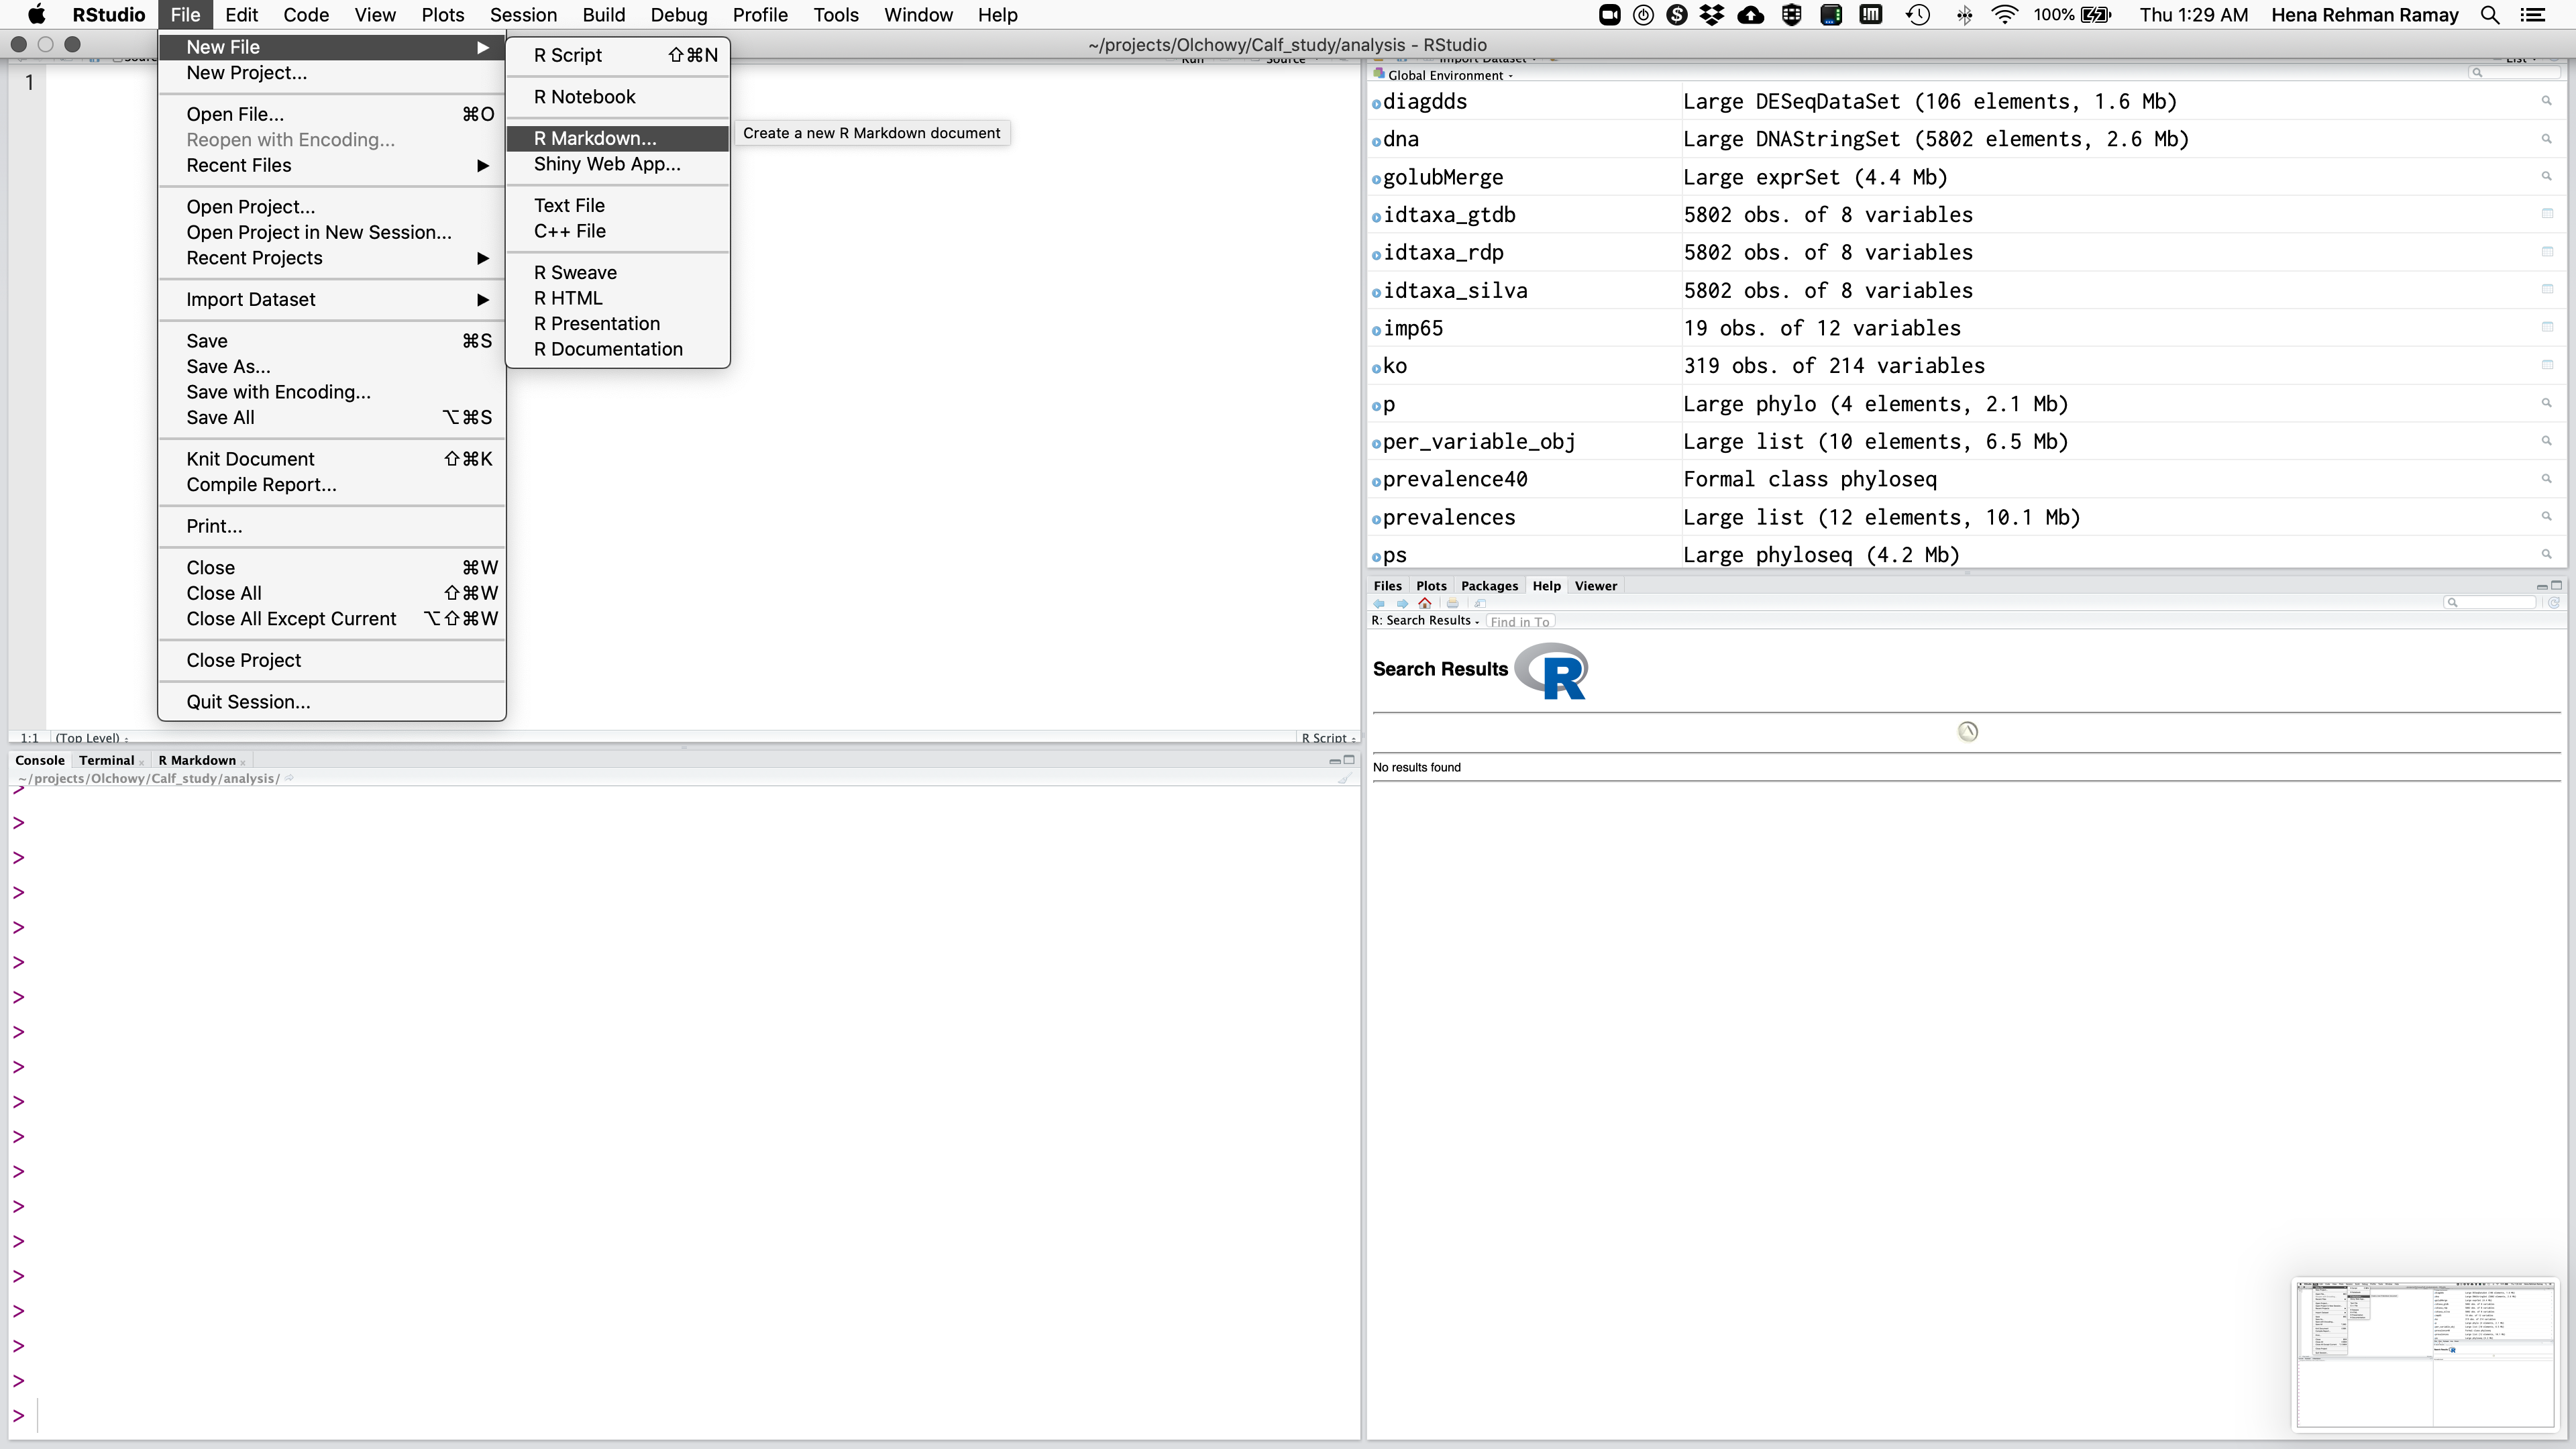
\includegraphics{img/markdown.png}

A screen will pop up asking us what kind of document we wish to create. Let's name our demo report ``Trial Report'' and fill in your name. Ensure that ``Document'' is highlighted to the left and that ``HTML'' is chosen. Click ``Ok''.

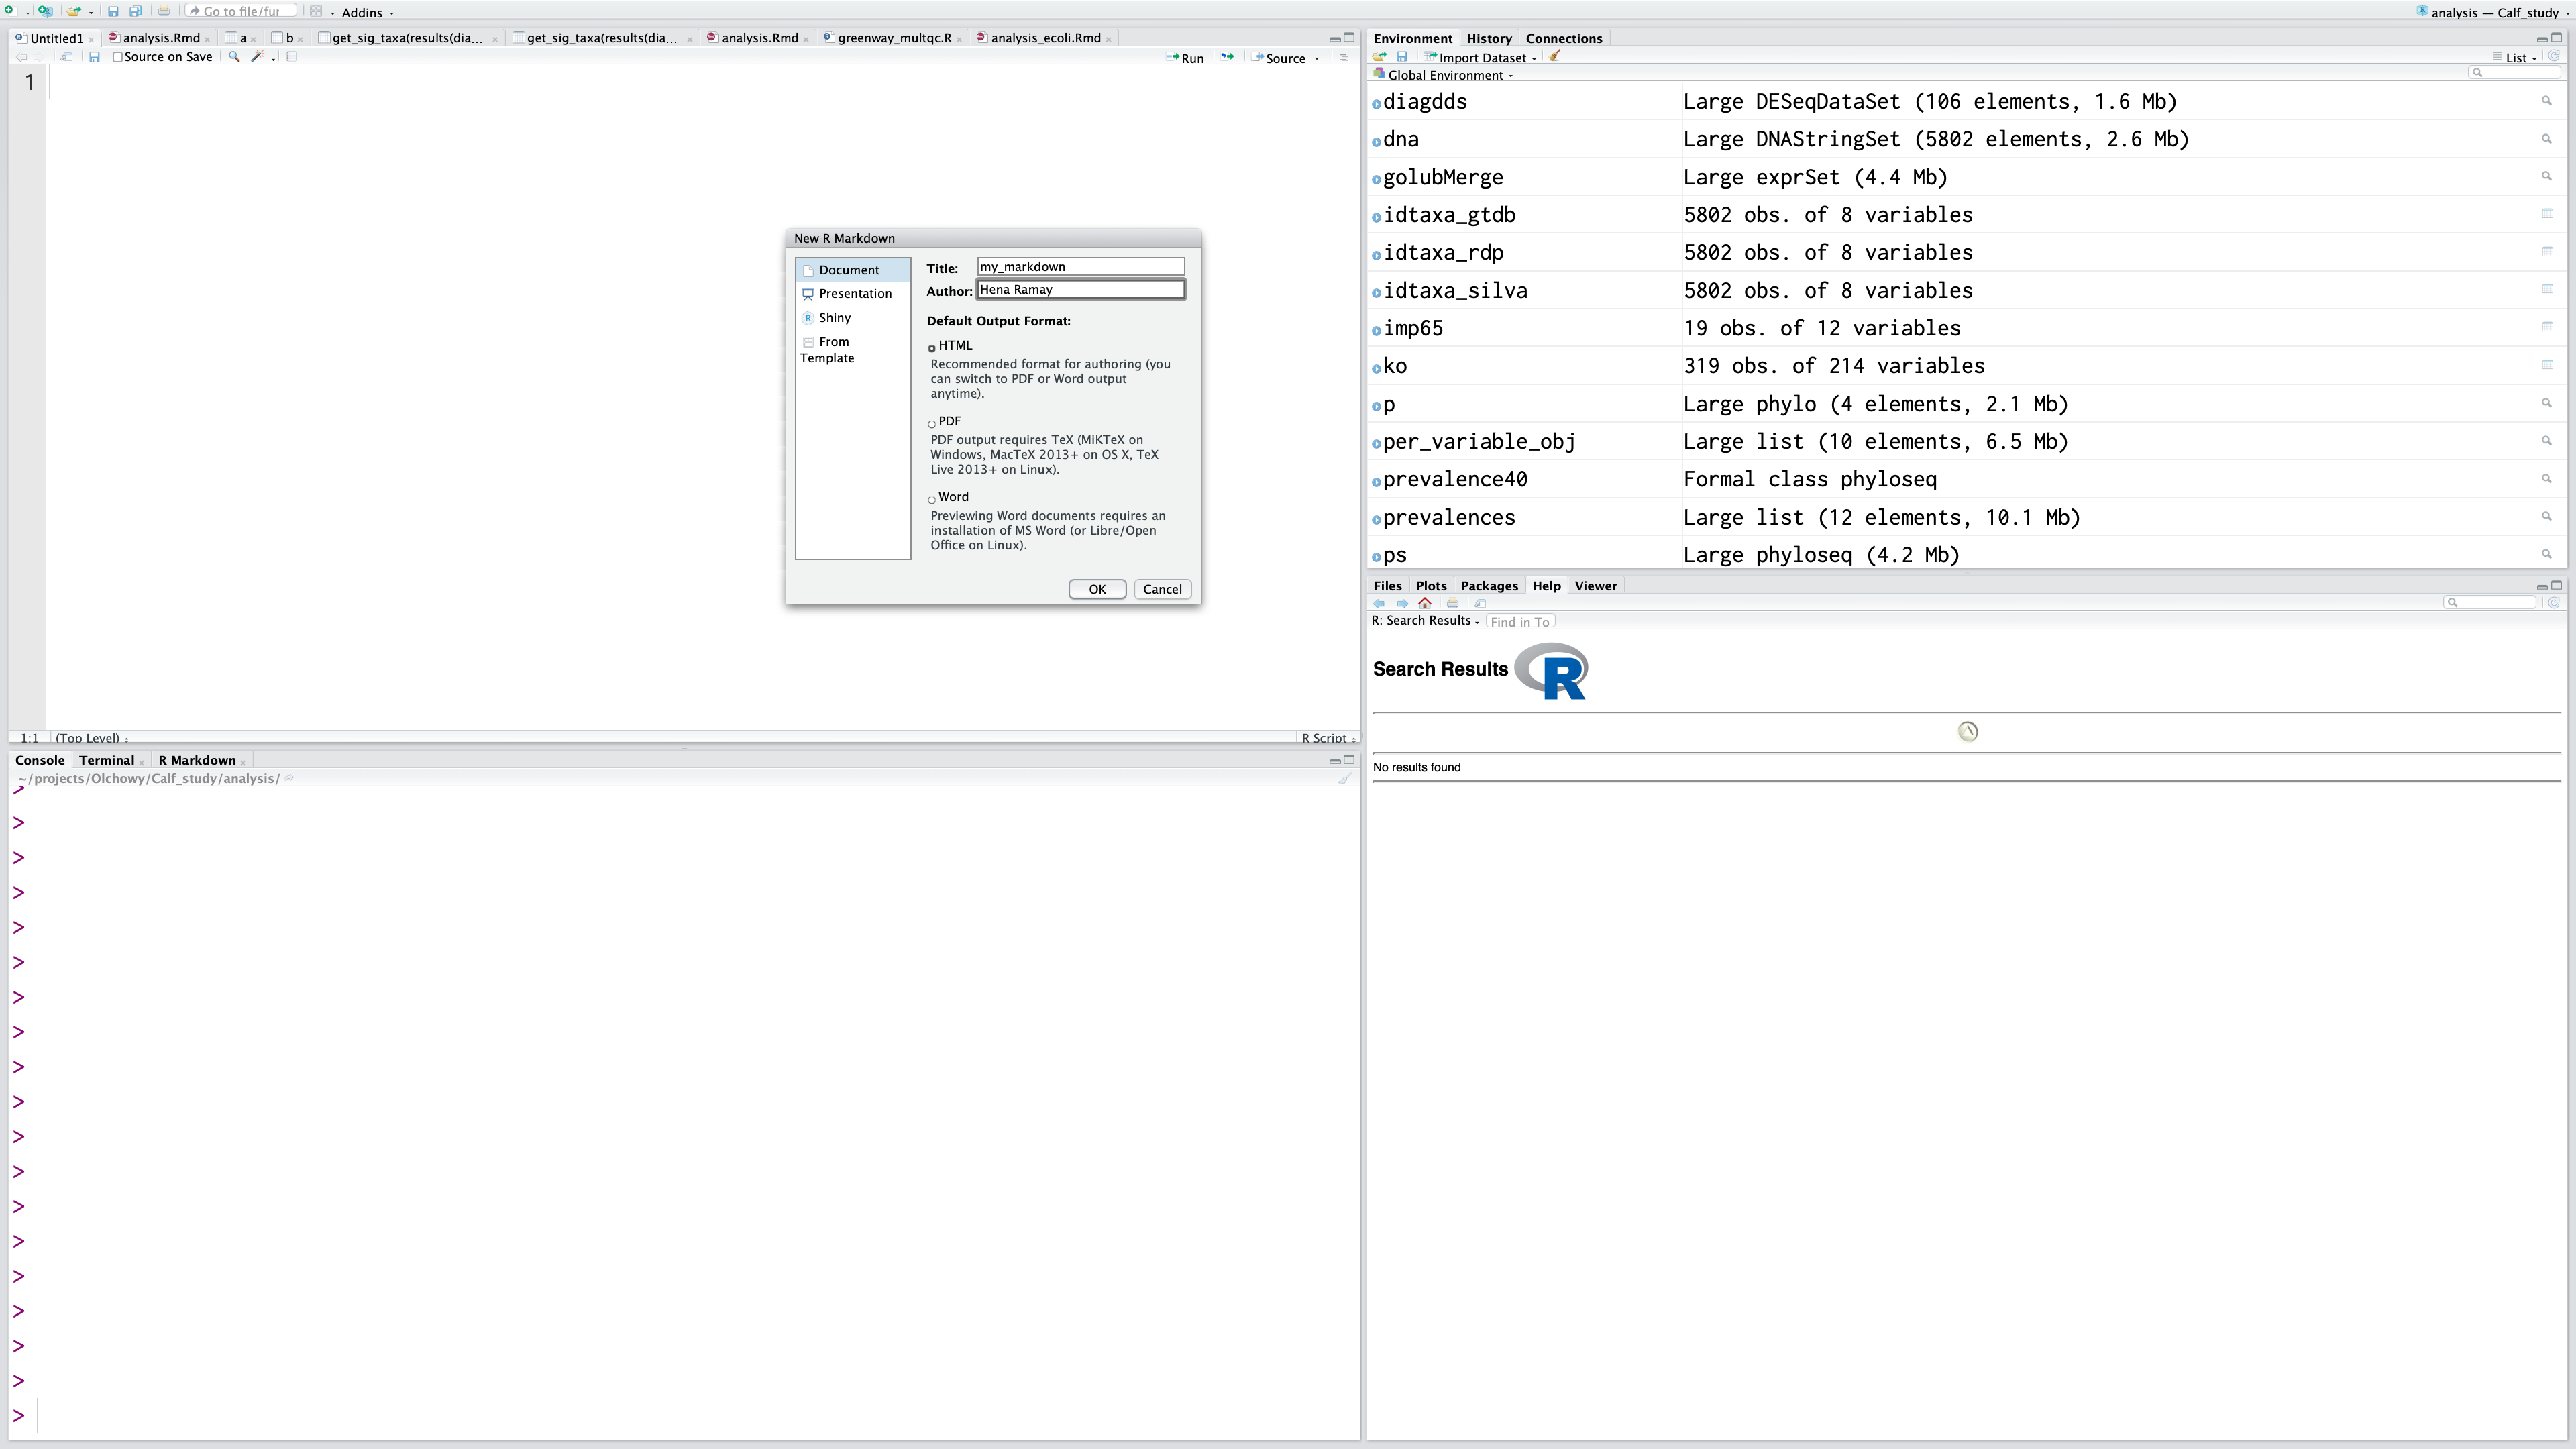
\includegraphics{img/mdname.png}

Now we have the example R Markdown file open. The first thing you'll notice at the top is a header which includes your name, the title of the document, the date, and a field called output. This header tells the package rmarkdown some information it might need about your document, including what format you want the final report rendered in.

The next thing you'll notice is white space with some text describing an R Markdown document. White space in this document represents text of the report you would like to display. You can put anything here describing your analysis, results, etc. and it will be recognized as text and not R code. This white space is interpreted as Markdown language, so you can use any of the tricks we learned in the last lesson to make lists, bold certain words, or create headers in your document.

In this trial script, you'll see how some of these markdown elements are used. For example, the word knit is in bolded (using asterisks), and there are code chucks near the bottom that say echo = FALSE.

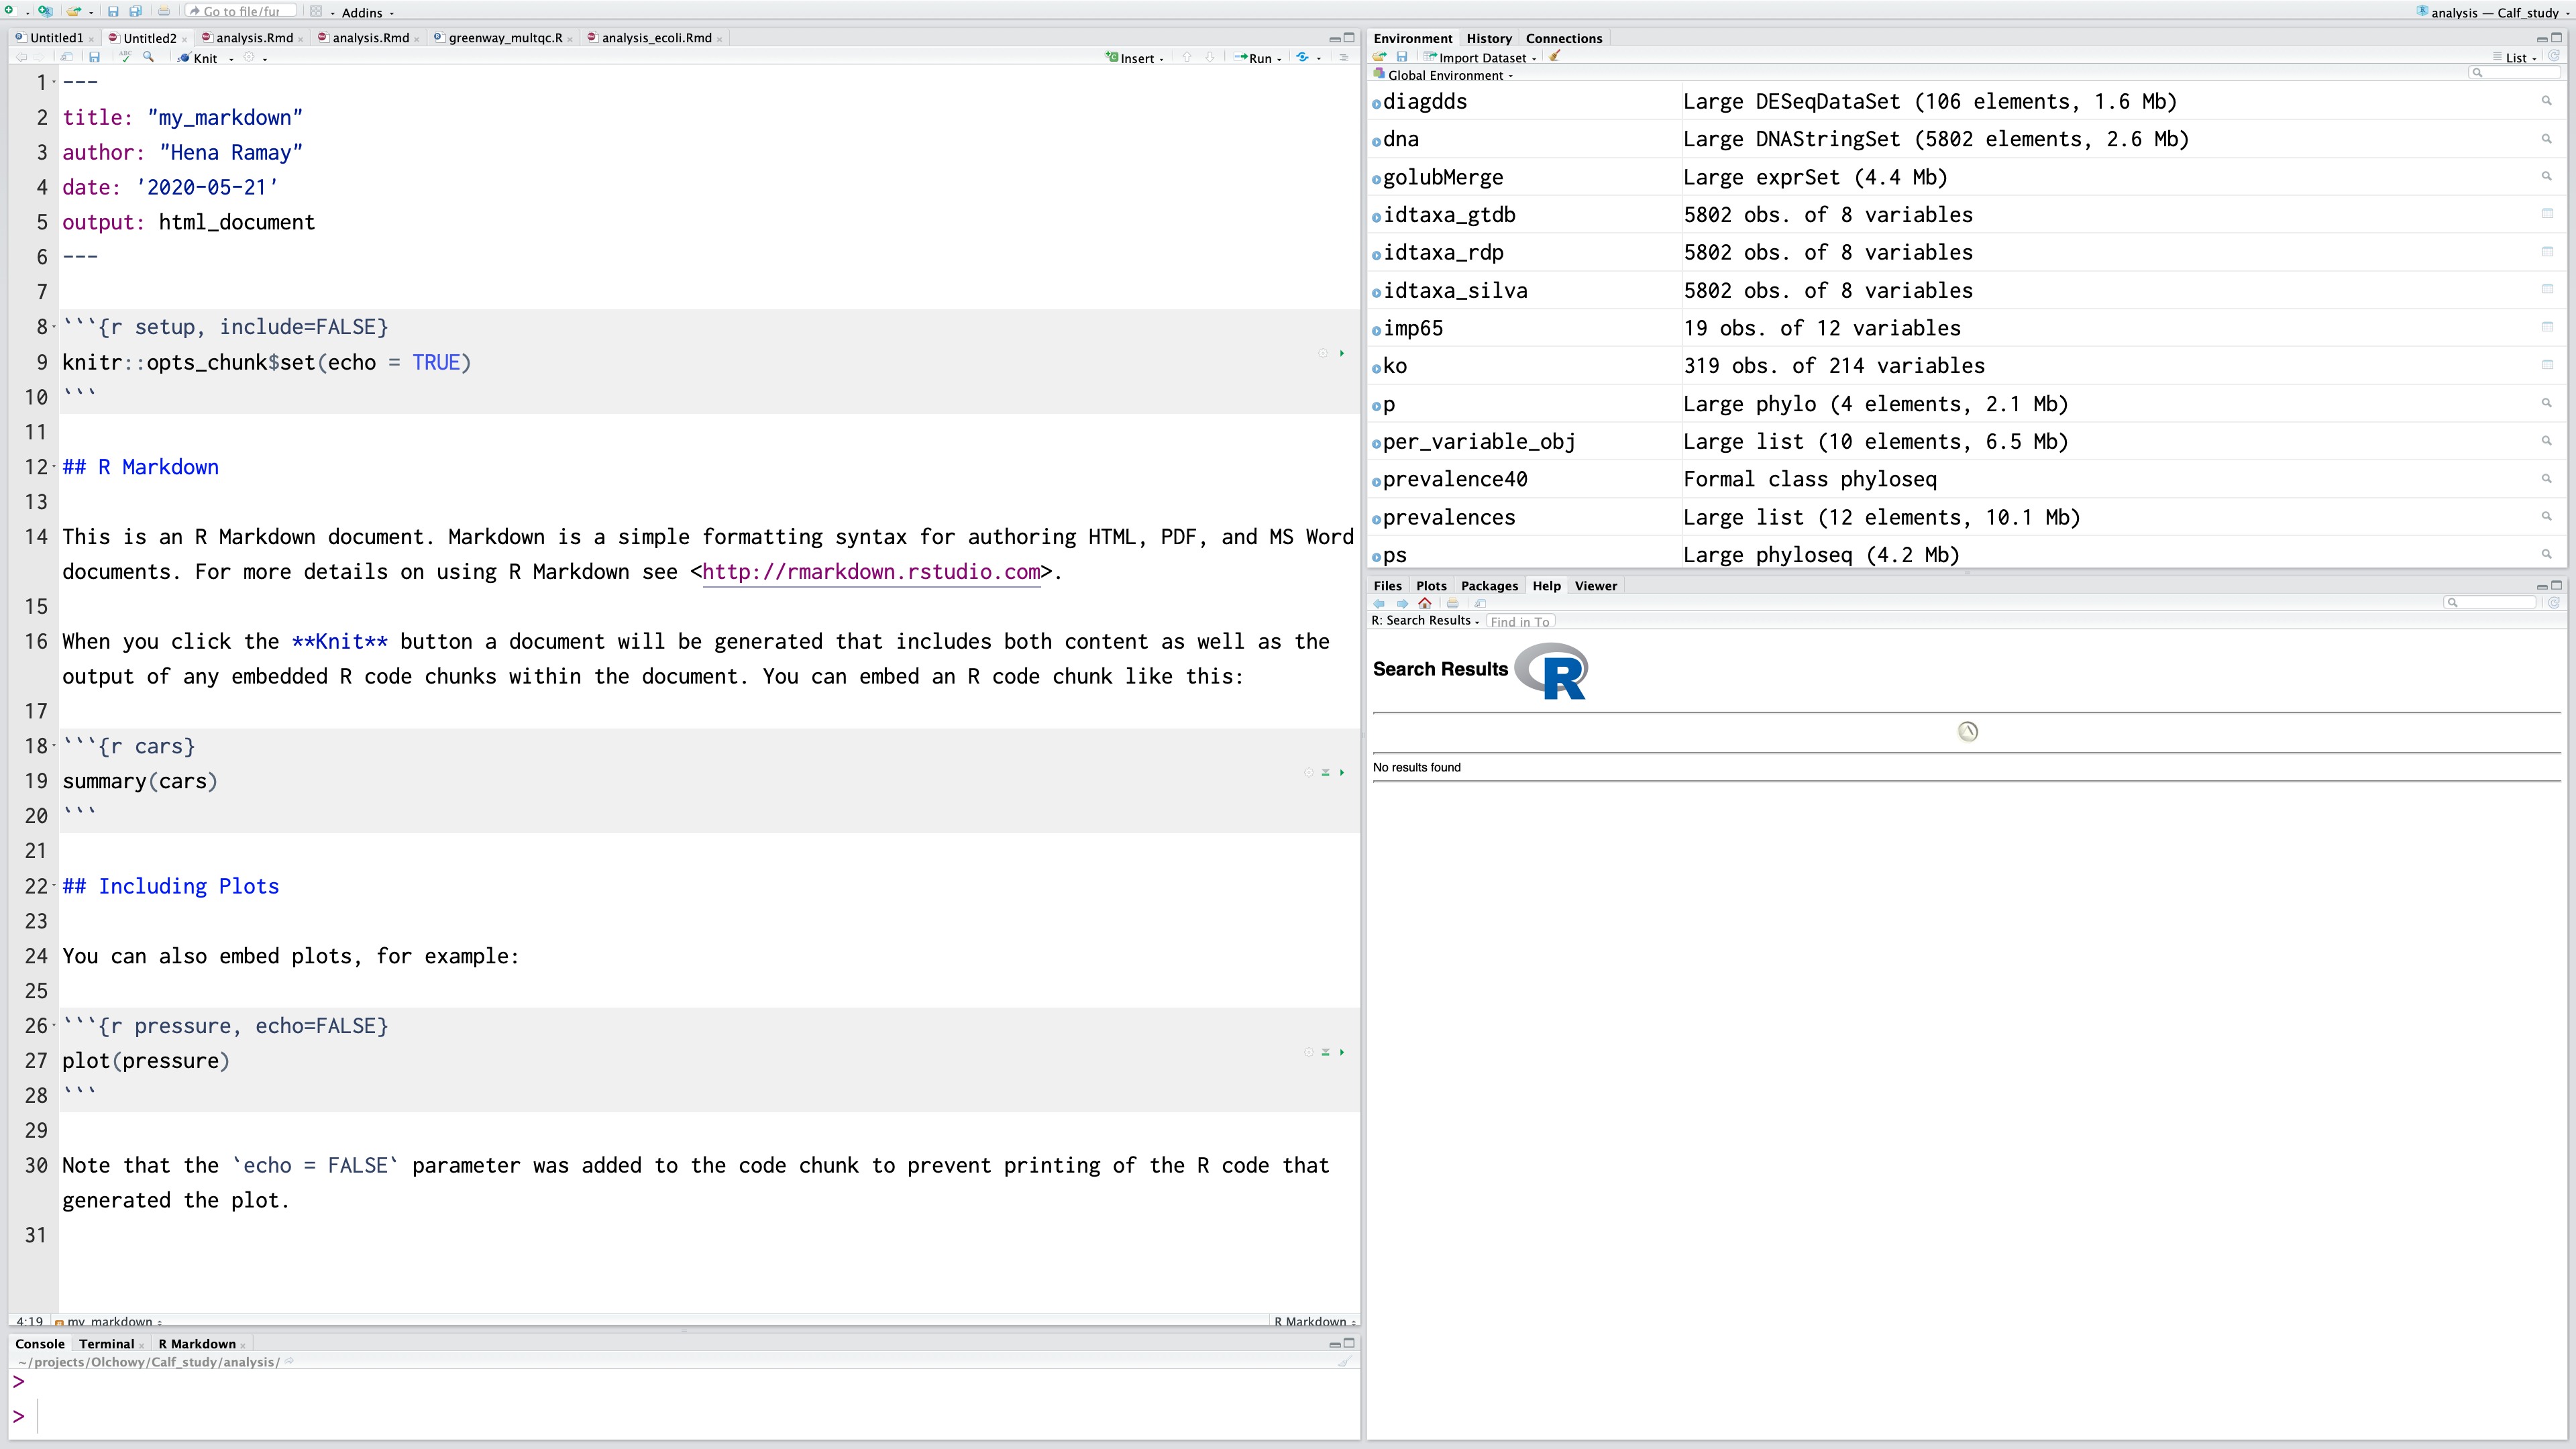
\includegraphics{img/firstmd.png}

\hypertarget{r-markdown-componenets}{%
\subsection{R Markdown componenets}\label{r-markdown-componenets}}

Notice that the file contains three types of content:

\begin{enumerate}
\def\labelenumi{\arabic{enumi}.}
\tightlist
\item
  An (optional) YAML header surrounded by ---s
\item
  R code chunks surrounded by ```s
\item
  text mixed with simple text formatting
\end{enumerate}

In addition to the white space, you'll gray blocks that have ``` at the top and bottom. These are called chunks. If the start of a chunk has \{r\} at the end of the ticks, the code will be run and both it and its output will be displayed in the rendered HTML. In your R Markdown, the code will look like:

In your final report, the code will look like:

\begin{verbatim}
summary(cars)
\end{verbatim}

Let's add a new chunk to end this demo document. To do so, either you can enter three backticks in a row, followed by \{r\}, or you can click on the green \texttt{Chunks}button and chose\texttt{Insert\ Chunk}. Additionally, there's a keyboard short cut which is \texttt{ctrl}+\texttt{alt}+\texttt{i}which will also pop up a chunk in an R Markdown document.

In the chunk, let's just examine the dimensions of the \texttt{car}mdataset:

You can actually send the code straight from the chunks over to console to be evaluated in two ways. First, you can highlight the code you want to run in the chunk and hit the \texttt{Run} button, which is located in the top right corner of the pane.

\hypertarget{knit-r-markdown}{%
\subsection{Knit R Markdown}\label{knit-r-markdown}}

These are the basics of writing R Markdown, but we still need to generate a report. To do this, click on the button on the top bar that says ``Knit HMTL''. This will prompt you to save the file. Go ahead and save this file as \texttt{Rmarkdown\_demo.Rmd} in the altmetrics directory. The ending of the file \texttt{.Rmd} indicates that this is an R Markdown file.

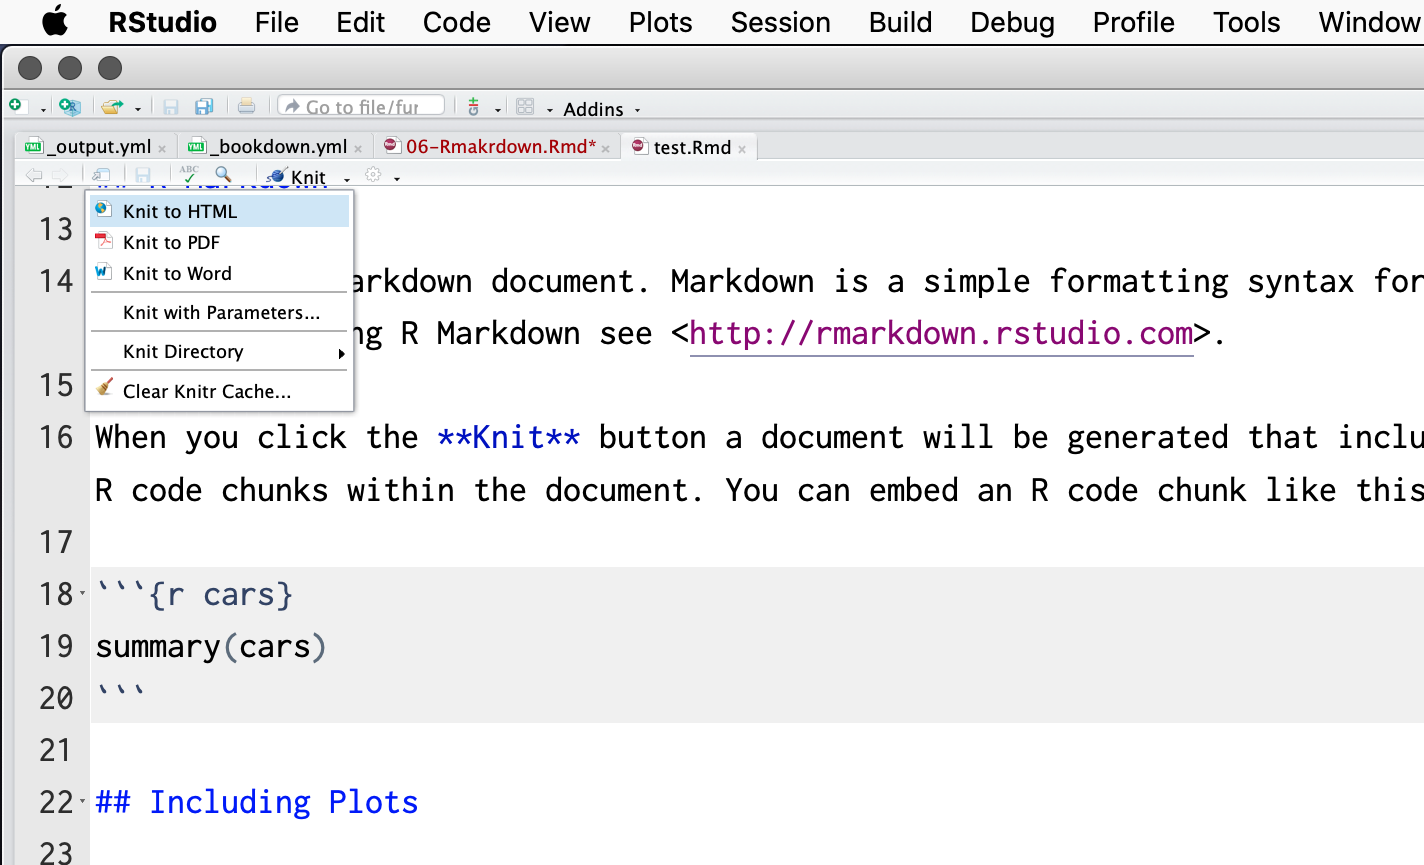
\includegraphics{img/kh.png}

When you click on this link, you see in the console that RStudio is running and rendering your R Markdown file. What is actually happening is RStudio is running the function \texttt{render}, which is part of the rmarkdown package. There are two things the command \texttt{render} does. First, it converts the R Markdown file to a Markdown file using the command \texttt{knit} from the knitr package (hence why rendering is called knitting). The second step is then the Markdown file is converted to the final file format (HTML, PDF, or Word).

The final result is that an HMTL file will pop up where you'll see the report. You can see the header has been rendered, there are code and results chunks displayed, and even plots are shown right in the report.

Also, if you now look in the altmetrics folder, you'll see an HTML file of the name Rmarkdown\_demo.html. When \texttt{render} is run, it saves the current version of the .Rmd file and the generated HTML file in the directory it is stored in.

\hypertarget{exercise}{%
\subsubsection*{Exercise}\label{exercise}}
\addcontentsline{toc}{subsubsection}{Exercise}

\begin{enumerate}
\def\labelenumi{\arabic{enumi}.}
\tightlist
\item
  Create a new project for this workshop.
\item
  In this project create a new markdown file called rworkshop.Rmd
\item
  Change the name of author to yours.
\item
  Click on the settings icon next to the knit button and go to output options. Try different themes and see how it changes you html output. Chose a theme that you like!
\end{enumerate}

\hypertarget{knitr-chunk-options}{%
\section{Knitr Chunk Options}\label{knitr-chunk-options}}

\hypertarget{learning-objectives-1}{%
\subsubsection*{Learning Objectives}\label{learning-objectives-1}}
\addcontentsline{toc}{subsubsection}{Learning Objectives}

Learn how to format chunks in R Markdown to display only the information you want to display.

You've learned the basics of how to incorporate markdown syntax with code chunks in an R Markdown file. Let's explore some additional options for making your code chunks appear the way you want them to appear in your reports. There are many ways to customize your chunks and you can explore all of the options by examining the \href{http://yihui.name/knitr/options/\#chunk_options}{documentation}. Here, we'll introduce you to some of the most useful options that you might use frequently.

Chunk output can be customized with~\href{http://yihui.name/knitr/options/}{knitr options ⧉}, arguments set in the~\texttt{\{\}}~of a chunk header. Above, we use five arguments:

\begin{itemize}
\tightlist
\item
  \texttt{include\ =\ FALSE}~prevents code and results from appearing in the finished file. R Markdown still runs the code in the chunk, and the results can be used by other chunks.
\item
  \texttt{echo\ =\ FALSE}~prevents code, but not the results from appearing in the finished file. This is a useful way to embed figures.
\item
  \texttt{message\ =\ FALSE}~prevents messages that are generated by code from appearing in the finished file.
\item
  \texttt{warning\ =\ FALSE}~prevents warnings that are generated by code from appearing in the finished.
\item
  \texttt{fig.cap\ =\ "..."}~adds a caption to graphical results.
\end{itemize}

The first thing you may want to consider is naming your code chunks, which makes degubbing easier, especially if you have a long script. Chunk names must be unique to each chunk.

Write the name of your chunk after the \{r\}, like: \texttt{\{r\ chunk\_name\}}

R Markdown:

Rendered:

\begin{Shaded}
\begin{Highlighting}[]
\KeywordTok{summary}\NormalTok{(cars)}
\end{Highlighting}
\end{Shaded}

\begin{verbatim}
##      speed           dist       
##  Min.   : 4.0   Min.   :  2.00  
##  1st Qu.:12.0   1st Qu.: 26.00  
##  Median :15.0   Median : 36.00  
##  Mean   :15.4   Mean   : 42.98  
##  3rd Qu.:19.0   3rd Qu.: 56.00  
##  Max.   :25.0   Max.   :120.00
\end{verbatim}

You can use RStudio to navigate to chunks based on their names, which can be especially useful as your script gets long. Click on the bottom left bar where it says \texttt{(Top\ Level)} and you'll see all of the chunk names in your script appear. Additionally, naming your chunks will be beneficial to identify errors in your code or slow sections when knitting your report.

Sometimes you may not want to see the code that produced a particular result in your report. You can have codeblocks in your R Markdown that are evaluated, but the code is not displayed in the final report by including \texttt{echo=FALSE} after the \texttt{\{r\ chunk\_name\}}.

R Markdown:

Rendered:

\begin{verbatim}
##      speed           dist       
##  Min.   : 4.0   Min.   :  2.00  
##  1st Qu.:12.0   1st Qu.: 26.00  
##  Median :15.0   Median : 36.00  
##  Mean   :15.4   Mean   : 42.98  
##  3rd Qu.:19.0   3rd Qu.: 56.00  
##  Max.   :25.0   Max.   :120.00
\end{verbatim}

Conversely, sometimes you may want to see the code, but not the output once the code is evalutated. To do so, you can include \texttt{results="hide"} after the chunk\_name:

R Markdown:

Rendered:

\begin{Shaded}
\begin{Highlighting}[]
\KeywordTok{summary}\NormalTok{(cars)}
\end{Highlighting}
\end{Shaded}

Sometimes, you may want to write a report where both the code and the output are suppressed. Why would you want to do that? Perhaps you're sending a report to a collaborator and you only want them to see the final figures, but not any data manipulation steps in the middle. To include a chunk that is evaluated, but no output is displayed - neither the code nor the results - put \texttt{include=FALSE} after the chunk\_name:

R Markdown:

Rendered (I swear there's a chunk after this! It's just invisible!):

There are tons of other options you can include in your chunks: sizing your figures and whether or not to display error or warning messages. As you write reports of your own data analysis, you can look up these options to create a report formatted in the way you want.

In addition to code chunks, you may want to include the results of an evaluation in line with regular text. For instance, you may want to describe the data in a paragraph, and include the number of individuals in that paragraph. To do so, you can indicate that a code box should be evaluated as R by including a lowercase r.

R Markdown:

\begin{verbatim}
The _cars_ dataset included in this analysis contains records for `r dim(cars)[1]` cars. 
\end{verbatim}

Rendered:

\begin{verbatim}
The _cars_ dataset included in this analysis contains records for 50 cars.
\end{verbatim}

\hypertarget{exercise-1}{%
\subsubsection*{Exercise}\label{exercise-1}}
\addcontentsline{toc}{subsubsection}{Exercise}

Now that you are familiar with chunks, create a chunk in which you do sum=1+1. Now by searching on the web, how can you re-use this chunk later in your rmd file.

\hypertarget{conditionals-and-loops}{%
\chapter{Conditionals and Loops}\label{conditionals-and-loops}}

\begin{center}\rule{0.5\linewidth}{0.5pt}\end{center}

\hypertarget{setup}{%
\section{Setup}\label{setup}}

\textbf{1. Download data.}

We will be using a dataset containing citation and alternative metrics for articles published in the PLOS family of journals between 2003 and 2010. The data set was compiled by Priem et al 2012 (\href{http://arxiv.org/abs/1203.4745}{publication}).

Download the data onto your computer from \href{https://www.dropbox.com/s/up38z3fd4llanrb/counts-raw.txt?dl=0}{this} dropbox link and move it into a directory on your computer that makes sense.

\textbf{2. Read in data into R.}

\begin{Shaded}
\begin{Highlighting}[]
\NormalTok{counts <-}\StringTok{ }\KeywordTok{read.delim}\NormalTok{(}\StringTok{"data/counts-raw.txt"}\NormalTok{)}
\end{Highlighting}
\end{Shaded}

\hypertarget{conditional-statements}{%
\section{Conditional statements}\label{conditional-statements}}

Decision making is an important part of programming. This can be achieved in R programming using conditional statements such as \texttt{if} and \texttt{if...else}.

\hypertarget{if}{%
\subsection*{if}\label{if}}
\addcontentsline{toc}{subsection}{if}

The syntax of an if statement is:

\begin{Shaded}
\begin{Highlighting}[]
\ControlFlowTok{if}\NormalTok{ (test_expression) \{}
\NormalTok{  do_this}
\NormalTok{\}}
\end{Highlighting}
\end{Shaded}

\begin{Shaded}
\begin{Highlighting}[]
\NormalTok{x <-}\StringTok{ }\DecValTok{5}
\ControlFlowTok{if}\NormalTok{ (x }\OperatorTok{>}\StringTok{ }\DecValTok{0}\NormalTok{) \{}
  \KeywordTok{print}\NormalTok{(}\StringTok{"positive number"}\NormalTok{)}
\NormalTok{\}}
\end{Highlighting}
\end{Shaded}

\begin{verbatim}
## [1] "positive number"
\end{verbatim}

\hypertarget{ifelse}{%
\subsection*{if\ldots else}\label{ifelse}}
\addcontentsline{toc}{subsection}{if\ldots else}

The syntax of an if\ldots else statement is:

\begin{Shaded}
\begin{Highlighting}[]
\ControlFlowTok{if}\NormalTok{ (test_expression) \{}
\NormalTok{  do_this}
\NormalTok{\} }\ControlFlowTok{else}\NormalTok{ \{}
\NormalTok{    do_that}
\NormalTok{\}}
\end{Highlighting}
\end{Shaded}

The else part is optional and is only evaluated if test\_expression is FALSE. It is important that the \texttt{else} word be in the same line as the closing brace of the \texttt{if} statement.

\begin{Shaded}
\begin{Highlighting}[]
\NormalTok{x <-}\StringTok{ }\DecValTok{1}
\ControlFlowTok{if}\NormalTok{ (x }\OperatorTok{>}\StringTok{ }\DecValTok{0}\NormalTok{)\{}
  \KeywordTok{print}\NormalTok{(}\StringTok{"positive number"}\NormalTok{)}
\NormalTok{\} }\ControlFlowTok{else}\NormalTok{ \{}
    \KeywordTok{print}\NormalTok{(}\StringTok{"negative number"}\NormalTok{)}
\NormalTok{\}}
\end{Highlighting}
\end{Shaded}

\begin{verbatim}
## [1] "positive number"
\end{verbatim}

\hypertarget{nested-ifelse-statements}{%
\subsection*{Nested if\ldots else statements}\label{nested-ifelse-statements}}
\addcontentsline{toc}{subsection}{Nested if\ldots else statements}

You can have more than two test expressions:

\begin{Shaded}
\begin{Highlighting}[]
\ControlFlowTok{if}\NormalTok{ (test_expression1) \{}
\NormalTok{  statement1}
\NormalTok{\} }\ControlFlowTok{else} \ControlFlowTok{if}\NormalTok{ (test_expression2) \{}
\NormalTok{    statement2}
\NormalTok{\} }\ControlFlowTok{else}\NormalTok{ \{}
\NormalTok{      statement4}
\NormalTok{\}}
\end{Highlighting}
\end{Shaded}

\begin{Shaded}
\begin{Highlighting}[]
\NormalTok{x <-}\StringTok{ }\DecValTok{0}
\ControlFlowTok{if}\NormalTok{ (x }\OperatorTok{<}\StringTok{ }\DecValTok{0}\NormalTok{) \{}
   \KeywordTok{print}\NormalTok{(}\StringTok{"negative number"}\NormalTok{)}
\NormalTok{\} }\ControlFlowTok{else} \ControlFlowTok{if}\NormalTok{ (x }\OperatorTok{>}\StringTok{ }\DecValTok{0}\NormalTok{) \{}
   \KeywordTok{print}\NormalTok{(}\StringTok{"positive number"}\NormalTok{)}
\NormalTok{\} }\ControlFlowTok{else}\NormalTok{ \{}
   \KeywordTok{print}\NormalTok{(}\StringTok{"zero"}\NormalTok{)}
\NormalTok{\}}
\end{Highlighting}
\end{Shaded}

\begin{verbatim}
## [1] "zero"
\end{verbatim}

\begin{center}\rule{0.5\linewidth}{0.5pt}\end{center}

\hypertarget{exercise-2.1}{%
\subsection*{EXERCISE 2.1}\label{exercise-2.1}}
\addcontentsline{toc}{subsection}{EXERCISE 2.1}

Write a simple if\ldots else statement to check if 5 is an odd number and if it is print ``I am odd'', otherwise print ``I am even''.

\begin{center}\rule{0.5\linewidth}{0.5pt}\end{center}

\hypertarget{loops}{%
\section{Loops}\label{loops}}

Conceptually, a loop is a way to repeat a sequence of instructions under certain conditions. They allow you to automate parts of your code that are in need of repetition.

\hypertarget{for-loop}{%
\subsection*{\texorpdfstring{\texttt{for} loop}{for loop}}\label{for-loop}}
\addcontentsline{toc}{subsection}{\texttt{for} loop}

The easiest and most frequently used loop in R is a for loop. Here is a demonstration of using loops.

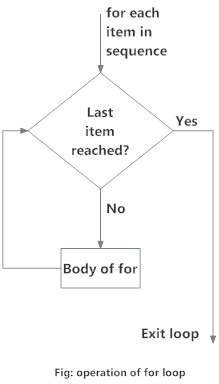
\includegraphics{img/r-for-loop.jpg}

\begin{Shaded}
\begin{Highlighting}[]
\NormalTok{year <-}\StringTok{ }\KeywordTok{c}\NormalTok{(}\DecValTok{2015}\NormalTok{,}\DecValTok{2016}\NormalTok{,}\DecValTok{2017}\NormalTok{,}\DecValTok{2018}\NormalTok{)}
\ControlFlowTok{for}\NormalTok{(i }\ControlFlowTok{in} \DecValTok{1}\OperatorTok{:}\KeywordTok{length}\NormalTok{(year)) \{}
  \KeywordTok{print}\NormalTok{(year[i])}
\NormalTok{\}}
\end{Highlighting}
\end{Shaded}

\begin{verbatim}
## [1] 2015
## [1] 2016
## [1] 2017
## [1] 2018
\end{verbatim}

\begin{Shaded}
\begin{Highlighting}[]
\ControlFlowTok{for}\NormalTok{(i }\ControlFlowTok{in} \DecValTok{1}\OperatorTok{:}\KeywordTok{length}\NormalTok{(year)) \{}
  \KeywordTok{print}\NormalTok{(}\KeywordTok{paste0}\NormalTok{(}\StringTok{"the year is "}\NormalTok{,year[i]))}
\NormalTok{\}}
\end{Highlighting}
\end{Shaded}

\begin{verbatim}
## [1] "the year is 2015"
## [1] "the year is 2016"
## [1] "the year is 2017"
## [1] "the year is 2018"
\end{verbatim}

\hypertarget{while-loop}{%
\subsection*{\texorpdfstring{\texttt{while} loop}{while loop}}\label{while-loop}}
\addcontentsline{toc}{subsection}{\texttt{while} loop}

In contrast to a \textbf{for} lop, \textbf{while} loops are used to loop until a specific conditional statement is no longer true.

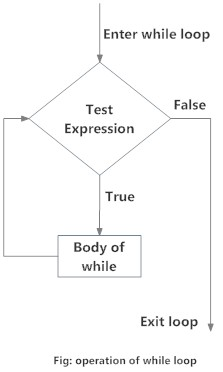
\includegraphics{img/r-while-loop.jpg}

\begin{Shaded}
\begin{Highlighting}[]
\ControlFlowTok{while}\NormalTok{ (test_expression) \{}
\NormalTok{  do_this}
\NormalTok{\}}
\end{Highlighting}
\end{Shaded}

\begin{Shaded}
\begin{Highlighting}[]
\NormalTok{i <-}\StringTok{ }\DecValTok{1}
\ControlFlowTok{while}\NormalTok{ (i }\OperatorTok{<}\StringTok{ }\DecValTok{6}\NormalTok{) \{}
  \KeywordTok{print}\NormalTok{(i)}
\NormalTok{  i <-}\StringTok{ }\NormalTok{i }\OperatorTok{+}\StringTok{ }\DecValTok{1}
\NormalTok{\}}
\end{Highlighting}
\end{Shaded}

\begin{verbatim}
## [1] 1
## [1] 2
## [1] 3
## [1] 4
## [1] 5
\end{verbatim}

\begin{center}\rule{0.5\linewidth}{0.5pt}\end{center}

\hypertarget{exercise-2.2}{%
\subsection*{EXERCISE 2.2}\label{exercise-2.2}}
\addcontentsline{toc}{subsection}{EXERCISE 2.2}

\textbf{Challenging.} From the PLOS journal publication data we read into R above, here is a plot showing the impact factor according to the F1000 (Faculty of 1000) versus the number of times the PDF was downloaded.

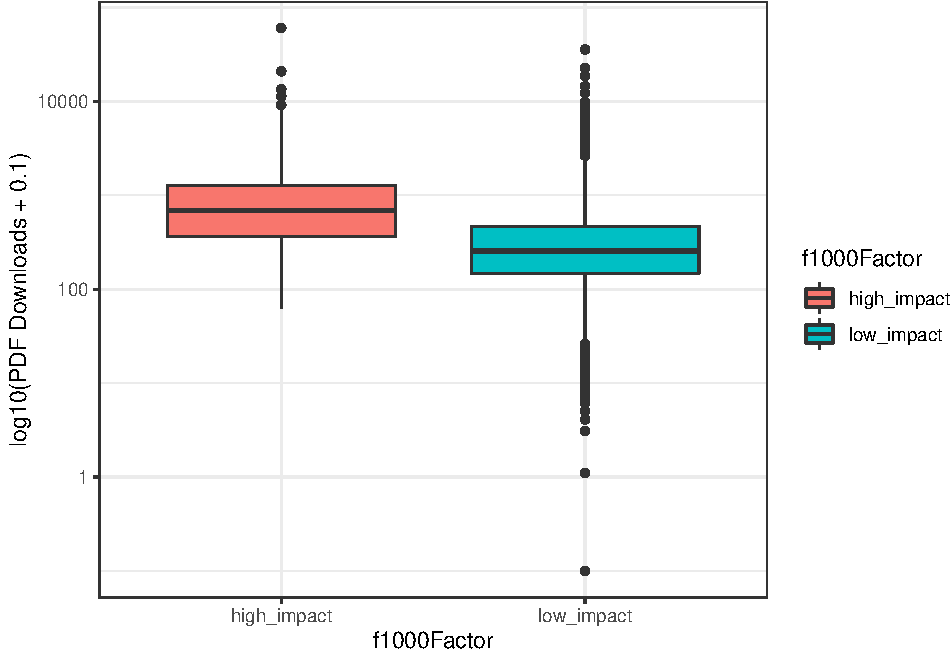
\includegraphics{Notes_files/figure-latex/unnamed-chunk-12-1.pdf}

Using this dataset, write a \texttt{for} loop containing an \texttt{if...else} statement to change the f1000Factor column into categorical variable with two levels: high impact and low impact.

Do this by translating the following sentence into R code: for every element in the f1000Factor variable, if the value is greater than zero, change it to ``high\_impact'', otherwise, change it to ``low\_impact''.

\textbf{Bonus.} Create a box plot (like the one below) showing the number of PDF downloads for high versus low impact articles.

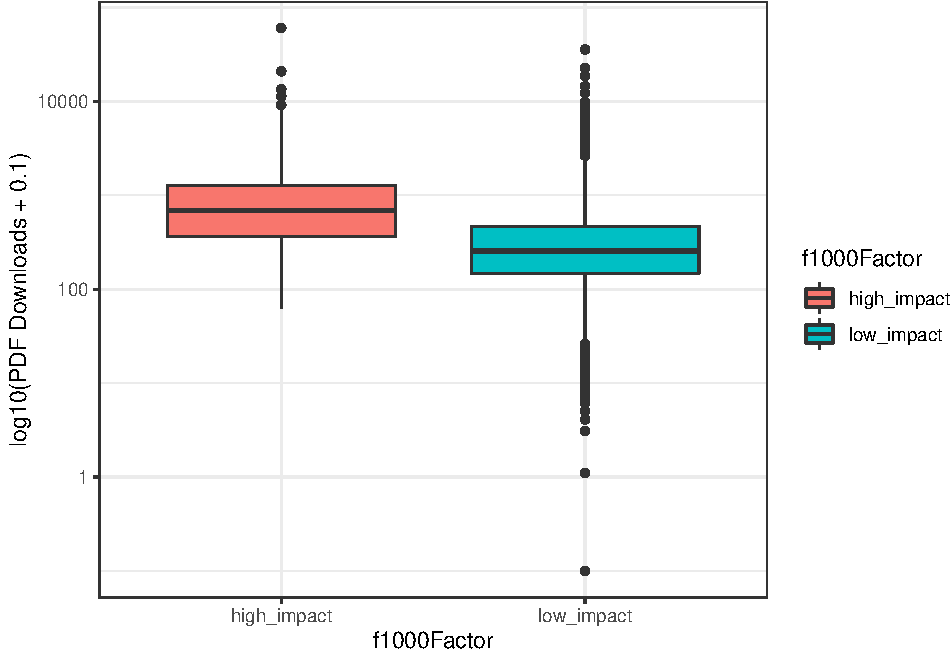
\includegraphics{Notes_files/figure-latex/unnamed-chunk-13-1.pdf}

\begin{center}\rule{0.5\linewidth}{0.5pt}\end{center}

\hypertarget{functions}{%
\chapter{Functions}\label{functions}}

``Intelligence is the ability to avoid doing work, yet getting the work done.''
― Linus Torvalds

\hypertarget{learning-objectives-2}{%
\subsubsection*{Learning Objectives}\label{learning-objectives-2}}
\addcontentsline{toc}{subsubsection}{Learning Objectives}

\begin{itemize}
\tightlist
\item
  Functions have two parts: arguments and body
\item
  Functions have their own environment
\item
  Functions help you repeat code chunks
\end{itemize}

In the last lesson we learnt to write loops to avoid writing the same code multiple time. Now lets learn how to make our code even more efficient and re-use the same code multiple times without copy-paste!

\hypertarget{parts-of-a-function}{%
\section{Parts of a function}\label{parts-of-a-function}}

We've already been using built-in R functions:~\texttt{read.csv},~\texttt{mean},~\texttt{length}, etc. These functions allow us to run the same routine with different inputs.

Let's explore~\texttt{read.csv}~further. All functions in R have two parts: the input arguments and the body. We can see the arguments of a function with the~\texttt{args}.

\begin{verbatim}
args(read.csv)
\end{verbatim}

\begin{verbatim}
function (file, header = TRUE, sep = ",", quote = "\"", dec = ".", 
    fill = TRUE, comment.char = "", ...) 
NULL
\end{verbatim}

So when we pass a character vector like~\texttt{"data/counts-raw."}, this gets assigned to the argument~\texttt{file}. All the other arguments have defaults set, so we do not need to assign them a value.

After the arguments have been assigned values, then the body of the function is executed. We can view the body of a function with~\texttt{body}.

\begin{verbatim}
body(read.csv)
\end{verbatim}

\begin{verbatim}
read.table(file = file, header = header, sep = sep, quote = quote,
    dec = dec, fill = fill, comment.char = comment.char, ...)
\end{verbatim}

\texttt{read.csv}~is very short. It just calls another function,~\texttt{read.table}, using the input file and the default arguments as the arguments passed to~\texttt{read.table}.

When we define our own functions, we use the syntax below. We list the arguments, separated by commas, within the parentheses. The body follows, contained within curly brackets~\texttt{\{\}}.

\begin{verbatim}
function_name <- function(args) {
  body
}
\end{verbatim}

\hypertarget{the-principle-of-encapsulation}{%
\section{The principle of encapsulation}\label{the-principle-of-encapsulation}}

An important feature of functions is the principle of encapsulation: the environment inside the function is distinct from the environment outside the function. In other words, variables defined inside a function are separate from variables defined outside the function.

Here's an small example to demonstrate this idea. The function~\texttt{ex\_fun}~takes two input arguments,~\texttt{x}~and~\texttt{y}. It calculates~\texttt{z}~and returns its value.

\begin{verbatim}
ex_fun <- function(x, y) {
  z <- x - y
  return(z)
}
\end{verbatim}

When we run~\texttt{ex\_fun}, the only thing returned to the global environment is the value that was assigned to~\texttt{z}. The variable~\texttt{z}~itself was only defined in the function environment, and does not exist in the global environment.

\begin{verbatim}
ex_fun(3, 10)
\end{verbatim}

\begin{verbatim}
[1] -7
\end{verbatim}

\begin{verbatim}
z
\end{verbatim}

\begin{verbatim}
Error in eval(expr, envir, enclos): object 'z' not found
\end{verbatim}

\hypertarget{environments}{%
\subsection{Environments}\label{environments}}

The situation presented above is a simplified version of environments which will serve you well if you treat functions as truly encapsulated. In reality, things are more complicated. For example, if inside a function you have a variable that has not been defined in the function, it will actually search the global environment for this variable. To learn the advanced details, see the chapter~\href{http://adv-r.had.co.nz/Environments.html}{Environments}~in Advanced R by Hadley Wickham.

\hypertarget{the-return-statement}{%
\section{The return statement}\label{the-return-statement}}

R provides the shortcut of not needing to use~\texttt{return}~at the end of the function. Instead, the variable on the last line of the body of the function is returned. This is useful for writing very small functions, but in these lessons we will use~\texttt{return}~to be more explicit about what is happening.

\hypertarget{exercise-2}{%
\subsubsection*{Exercise}\label{exercise-2}}
\addcontentsline{toc}{subsubsection}{Exercise}

\begin{enumerate}
\def\labelenumi{\arabic{enumi}.}
\tightlist
\item
  Write your own function called~\texttt{select\_first}. It should take a vector as input and return the first element of the list.
  s
\item
  Now use articleType column from counts dataframe and use it as input to select\_first function.
\item
  Now create a function called `select\_el' which takes two arguments, a vector and an index. It should return the value in the index of the vector. For example if I give it a vector x=(10,22,49) and index=2, it should return 22.
  select\_el(x,index)
\item
  Now add to select\_el funciton some code that will spit out an error if the index \textgreater{} length(x). Hint you can use if statement and stop() function.
\end{enumerate}

\hypertarget{the-apply-family}{%
\chapter{The apply family}\label{the-apply-family}}

\hypertarget{learning-objectives-3}{%
\subsubsection*{Learning Objectives}\label{learning-objectives-3}}
\addcontentsline{toc}{subsubsection}{Learning Objectives}

Learn to use apply family functions in place of loops.

Whenever you're using a for loop, you might want to revise your code and see whether you can use the lapply function instead. Learn all about this intuitive way of applying a function over a list or a vector, and its variants sapply and vapply.

\hypertarget{apply}{%
\section{apply()}\label{apply}}

apply() takes Data frame or matrix as an input and gives output in vector, list or array. apply() Function is primarily used to avoid explicit uses of loop constructs. It is the most basic of all collections can be used over a matrice.

This function takes 3 arguments:

\begin{verbatim}
apply(X, MARGIN, FUN)
\end{verbatim}

apply() takes an array or matrix \texttt{X}, a \texttt{Margin} that takes a value 1 for rows or 2 for columns and applies a functoin \texttt{FUN} to it.

\begin{Shaded}
\begin{Highlighting}[]
\NormalTok{m1 <-}\StringTok{ }\KeywordTok{matrix}\NormalTok{(C<-(}\DecValTok{1}\OperatorTok{:}\DecValTok{10}\NormalTok{),}\DataTypeTok{nrow=}\DecValTok{5}\NormalTok{, }\DataTypeTok{ncol=}\DecValTok{6}\NormalTok{)}
\NormalTok{m1}
\end{Highlighting}
\end{Shaded}

\begin{verbatim}
##      [,1] [,2] [,3] [,4] [,5] [,6]
## [1,]    1    6    1    6    1    6
## [2,]    2    7    2    7    2    7
## [3,]    3    8    3    8    3    8
## [4,]    4    9    4    9    4    9
## [5,]    5   10    5   10    5   10
\end{verbatim}

\begin{Shaded}
\begin{Highlighting}[]
\NormalTok{a_m1 <-}\StringTok{ }\KeywordTok{apply}\NormalTok{(m1, }\DecValTok{2}\NormalTok{, sum)}
\NormalTok{a_m1}
\end{Highlighting}
\end{Shaded}

\begin{verbatim}
## [1] 15 40 15 40 15 40
\end{verbatim}

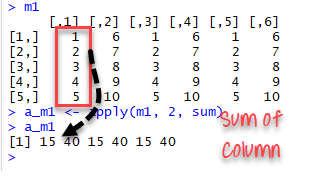
\includegraphics{img/apply.png}

\hypertarget{exercise-3}{%
\subsubsection*{Exercise}\label{exercise-3}}
\addcontentsline{toc}{subsubsection}{Exercise}

Select the columns from count.raw file from pdfDownloadsCount to hmtlDownloadsCount and using the apply function find the mean of each column.

\hypertarget{lapply}{%
\section{lapply()}\label{lapply}}

Before you go about solving the exercises below, have a look at the documentation of the \texttt{lapply()} function. The Usage section shows the following expression:

\begin{verbatim}
lapply(X, FUN, ...)
\end{verbatim}

To put it generally, \texttt{lapply} takes a vector or list \texttt{X}, and applies the function \texttt{FUN} to each of its members. If \texttt{FUN} requires additional arguments, you pass them after you've specified \texttt{X} and \texttt{FUN} (\texttt{...}). The output of \texttt{lapply()} is a list, the same length as \texttt{X}, where each element is the result of applying \texttt{FUN} on the corresponding element of \texttt{X}.

Now that you are truly brushing up on your data science skills, let's revisit some of the most relevant figures in data science history. We've compiled a vector of famous mathematicians/statisticians and the year they were born. Up to you to extract some information!

\hypertarget{example}{%
\subsubsection{Example}\label{example}}

\begin{Shaded}
\begin{Highlighting}[]
\CommentTok{# The vector pioneers has already been created for you}
\NormalTok{pioneers <-}\StringTok{ }\KeywordTok{c}\NormalTok{(}\StringTok{"GAUSS:1777"}\NormalTok{, }\StringTok{"BAYES:1702"}\NormalTok{, }\StringTok{"PASCAL:1623"}\NormalTok{, }\StringTok{"PEARSON:1857"}\NormalTok{)}

\CommentTok{# Split names from birth year to make split_math a list}
\NormalTok{split_math <-}\StringTok{ }\KeywordTok{strsplit}\NormalTok{(pioneers, }\DataTypeTok{split =} \StringTok{":"}\NormalTok{)}
\CommentTok{# Convert to lowercase strings: split_low}
\NormalTok{split_low <-}\StringTok{ }\KeywordTok{lapply}\NormalTok{(split_math, tolower)}
\CommentTok{# Take a look at the structure of split_low}
\KeywordTok{str}\NormalTok{(split_low)}
\end{Highlighting}
\end{Shaded}

\begin{verbatim}
## List of 4
##  $ : chr [1:2] "gauss" "1777"
##  $ : chr [1:2] "bayes" "1702"
##  $ : chr [1:2] "pascal" "1623"
##  $ : chr [1:2] "pearson" "1857"
\end{verbatim}

\hypertarget{use-lapply-with-your-own-function}{%
\subsection{Use lapply with your own function}\label{use-lapply-with-your-own-function}}

You can use \texttt{lapply()} on your own functions as well. You just need to code a new function and make sure it is available in the workspace. After that, you can use the function inside \texttt{lapply()} just as you did with base R functions. We have already created a select\_first() function so lets apply it to a

\hypertarget{exercise-4}{%
\subsubsection*{Exercise}\label{exercise-4}}
\addcontentsline{toc}{subsubsection}{Exercise}

Use lapply on split\_low list and use the select\_first() function you created.

\hypertarget{lapply-and-anonymous-functions}{%
\subsection{lapply and anonymous functions}\label{lapply-and-anonymous-functions}}

Writing your own functions and then using them inside \texttt{lapply()} is quite an accomplishment! But defining functions to use them only once is kind of overkill, isn't it? That's why you can use so-called \textbf{anonymous functions} in R.

Previously, you learned that functions in R are objects in their own right. This means that they aren't automatically bound to a name. When you create a function, you can use the assignment operator to give the function a name. It's perfectly possible, however, to not give the function a name. This is called an anonymous function:

\begin{verbatim}
# Named function
select_first <- function(x) { x[1] }

# Use anonymous function inside lapply()
lapply(list(1,2,3), function(x) {x[1]})
\end{verbatim}

\hypertarget{example-1}{%
\subsubsection{Example}\label{example-1}}

\begin{Shaded}
\begin{Highlighting}[]
\CommentTok{# Transform: use anonymous function inside lapply}
\NormalTok{names <-}\StringTok{ }\KeywordTok{lapply}\NormalTok{(split_low, }\ControlFlowTok{function}\NormalTok{(x) \{ x[}\DecValTok{1}\NormalTok{] \})}
\end{Highlighting}
\end{Shaded}

\hypertarget{use-lapply-with-additional-arguments}{%
\subsection{Use lapply with additional arguments}\label{use-lapply-with-additional-arguments}}

In the video, the \texttt{triple()} function was transformed to the \texttt{multiply()} function to allow for a more generic approach. \texttt{lapply()} provides a way to handle functions that require more than one argument, such as the \texttt{multiply()} function:

\begin{verbatim}
multiply <- function(x, factor) {
  x * factor
}

lapply(list(1,2,3), multiply, factor = 3)
\end{verbatim}

On the right we've included a generic version of the select functions that you've coded earlier: \texttt{select\_el()}. It takes a vector as its first argument, and an index as its second argument. It returns the vector's element at the specified index.

\hypertarget{example-2}{%
\subsubsection{Example}\label{example-2}}

\begin{Shaded}
\begin{Highlighting}[]
\CommentTok{# Generic select function}
\NormalTok{select_el <-}\StringTok{ }\ControlFlowTok{function}\NormalTok{(x, index) \{}
\NormalTok{  x[index]}
\NormalTok{\}}
\CommentTok{# Use lapply() twice on split_low: names and years}
\NormalTok{names <-}\StringTok{ }\KeywordTok{lapply}\NormalTok{(split_low, select_el, }\DataTypeTok{index =} \DecValTok{1}\NormalTok{)}
\NormalTok{years <-}\StringTok{ }\KeywordTok{lapply}\NormalTok{(split_low, select_el, }\DataTypeTok{index =} \DecValTok{2}\NormalTok{)}
\end{Highlighting}
\end{Shaded}

\hypertarget{sapply}{%
\section{sapply()}\label{sapply}}

You can use \texttt{sapply()} similar to how you used \texttt{lapply()}. sapply is a user-friendly version and wrapper of lapply by default returning a vector, matrix .The first argument of \texttt{sapply()} is the list or vector \texttt{X} over which you want to apply a function, \texttt{FUN}. Potential additional arguments to this function are specified afterwards (\texttt{...}):

\begin{verbatim}
sapply(X, FUN, ...)
\end{verbatim}

\hypertarget{example-3}{%
\subsubsection{Example}\label{example-3}}

\begin{Shaded}
\begin{Highlighting}[]
\CommentTok{# Constructing temp variable}
\NormalTok{names <-}\StringTok{ }\KeywordTok{sapply}\NormalTok{(split_low, select_el, }\DataTypeTok{index =} \DecValTok{1}\NormalTok{)}
\end{Highlighting}
\end{Shaded}

\hypertarget{sapply-with-your-own-function}{%
\subsection{sapply with your own function}\label{sapply-with-your-own-function}}

Like \texttt{lapply()}, \texttt{sapply()} allows you to use self-defined functions and apply them over a vector or a list:

\begin{verbatim}
sapply(X, FUN, ...)
\end{verbatim}

Here, \texttt{FUN} can be one of R's built-in functions, but it can also be a function you wrote. This self-written function can be defined before hand, or can be inserted directly as an anonymous function.

\hypertarget{sapply-with-function-returning-vector}{%
\subsection{sapply with function returning vector}\label{sapply-with-function-returning-vector}}

In the previous exercises, you've seen how \texttt{sapply()} simplifies the list that \texttt{lapply()} would return by turning it into a vector. But what if the function you're applying over a list or a vector returns a vector of length greater than 1? If you don't remember from the video, don't waste more time in the valley of ignorance and head over to the instructions!

\hypertarget{example-4}{%
\subsubsection{Example}\label{example-4}}

\begin{Shaded}
\begin{Highlighting}[]
\NormalTok{temp=}\KeywordTok{list}\NormalTok{(}\KeywordTok{c}\NormalTok{(}\DecValTok{1}\NormalTok{,}\DecValTok{3}\NormalTok{,}\DecValTok{4}\NormalTok{,}\DecValTok{4}\NormalTok{,}\DecValTok{6}\NormalTok{),}\KeywordTok{c}\NormalTok{(}\DecValTok{3}\NormalTok{,}\DecValTok{4}\NormalTok{,}\DecValTok{6}\NormalTok{,}\DecValTok{8}\NormalTok{,}\DecValTok{9}\NormalTok{))}
\CommentTok{# Create a function that returns min and max of a vector: extremes}
\NormalTok{extremes <-}\StringTok{ }\ControlFlowTok{function}\NormalTok{(x) \{}
  \KeywordTok{c}\NormalTok{(}\DataTypeTok{min =} \KeywordTok{min}\NormalTok{(x), }\DataTypeTok{max =} \KeywordTok{max}\NormalTok{(x))}
\NormalTok{\}}
\CommentTok{# Apply extremes() over temp with lapply()}
\KeywordTok{lapply}\NormalTok{(temp, extremes)}
\end{Highlighting}
\end{Shaded}

\begin{verbatim}
## [[1]]
## min max 
##   1   6 
## 
## [[2]]
## min max 
##   3   9
\end{verbatim}

\begin{Shaded}
\begin{Highlighting}[]
\CommentTok{# Apply extremes() over temp with sapply()}
\KeywordTok{sapply}\NormalTok{(temp, extremes)}
\end{Highlighting}
\end{Shaded}

\begin{verbatim}
##     [,1] [,2]
## min    1    3
## max    6    9
\end{verbatim}

\hypertarget{sapply-cant-simplify-now-what}{%
\subsection{sapply can't simplify, now what?}\label{sapply-cant-simplify-now-what}}

It seems like we've hit the jackpot with \texttt{sapply()}. On all of the examples so far, \texttt{sapply()} was able to nicely simplify the rather bulky output of \texttt{lapply()}. But, as with life, there are things you can't simplify. How does \texttt{sapply()} react?

We already created a function, \texttt{below\_zero()}, that takes a vector of numerical values and returns a vector that only contains the values that are strictly below zero.

\hypertarget{example-5}{%
\subsubsection{Example}\label{example-5}}

\begin{Shaded}
\begin{Highlighting}[]
\CommentTok{# temp is already prepared for you in the workspace}
\CommentTok{# Definition of below_zero()}
\NormalTok{below_zero <-}\StringTok{ }\ControlFlowTok{function}\NormalTok{(x) \{}
  \KeywordTok{return}\NormalTok{(x[x }\OperatorTok{<}\StringTok{ }\DecValTok{0}\NormalTok{])}
\NormalTok{\}}
\CommentTok{# Apply below_zero over temp using lapply(): freezing_l}
\NormalTok{freezing_l <-}\StringTok{ }\KeywordTok{lapply}\NormalTok{(temp, below_zero)}
\CommentTok{# Apply below_zero over temp using sapply(): freezing_s}
\NormalTok{freezing_s <-}\StringTok{ }\KeywordTok{sapply}\NormalTok{(temp, below_zero)}
\CommentTok{# Are freezing_l and freezing_s identical?}
\KeywordTok{identical}\NormalTok{(freezing_l, freezing_s)}
\end{Highlighting}
\end{Shaded}

\begin{verbatim}
## [1] TRUE
\end{verbatim}

\hypertarget{vapply}{%
\section{vapply()}\label{vapply}}

Before you get your hands dirty with the third and last apply function that you'll learn about in this intermediate R course, let's take a look at its syntax. The function is called \texttt{vapply()}, and it has the following syntax:

\begin{verbatim}
vapply(X, FUN, FUN.VALUE, ..., USE.NAMES = TRUE)
\end{verbatim}

Over the elements inside \texttt{X}, the function \texttt{FUN} is applied. The \texttt{FUN.VALUE} argument expects a template for the return argument of this function \texttt{FUN}. \texttt{USE.NAMES} is \texttt{TRUE} by default; in this case \texttt{vapply()} tries to generate a named array, if possible.

For the next set of exercises, you'll be working on the \texttt{temp} list again, that contains 7 numerical vectors of length 5. We also coded a function \texttt{basics()} that takes a vector, and returns a named vector of length 3, containing the minimum, mean and maximum value of the vector respectively.

\hypertarget{example-6}{%
\subsubsection{Example}\label{example-6}}

\begin{Shaded}
\begin{Highlighting}[]
\CommentTok{# temp is already available in the workspace}
\CommentTok{# Definition of basics()}
\NormalTok{basics <-}\StringTok{ }\ControlFlowTok{function}\NormalTok{(x) \{}
  \KeywordTok{c}\NormalTok{(}\DataTypeTok{min =} \KeywordTok{min}\NormalTok{(x), }\DataTypeTok{mean =} \KeywordTok{mean}\NormalTok{(x), }\DataTypeTok{max =} \KeywordTok{max}\NormalTok{(x))}
\NormalTok{\}}
\CommentTok{# Apply basics() over temp using vapply()}
\KeywordTok{vapply}\NormalTok{(temp, basics, }\KeywordTok{numeric}\NormalTok{(}\DecValTok{3}\NormalTok{))}
\end{Highlighting}
\end{Shaded}

\begin{verbatim}
##      [,1] [,2]
## min   1.0    3
## mean  3.6    6
## max   6.0    9
\end{verbatim}

\hypertarget{exercise-5}{%
\subsubsection{Exercise}\label{exercise-5}}

\begin{verbatim}
<br>
Use the table() function and one of the apply functions to see how many counts of each year and articleType are available. 
Explain which function you used and what does the output look like?

</div>







<!--chapter:end:05-Apply_family.Rmd-->

# Advanced Plotting 

"The greatest value of a picture is when it forces us to notice what we never expected to see"
-John Tukey

---

## Setup

**1. Install the `tidyverse` package.**


```r
library(tidyverse)
\end{verbatim}

\textbf{2. Filter data.}

We will be using the publication dataset that we read into R in Chapter 2 as \texttt{counts}.

\begin{Shaded}
\begin{Highlighting}[]
\NormalTok{research <-}\StringTok{ }\KeywordTok{filter}\NormalTok{(counts, articleType }\OperatorTok{==}\StringTok{ "Research Article"}\NormalTok{)}
\end{Highlighting}
\end{Shaded}

\hypertarget{review-of-ggplot2-basics}{%
\section{Review of ggplot2 basics}\label{review-of-ggplot2-basics}}

\texttt{ggplot2} is a plotting package that makes it simple to create complex plots from data in a data frame. Graphics are built step by step by adding new elements. Adding layers in this fashion allows for extensive flexibility and customization of plots.

A plot can be divided into different fundamental parts:

\textbf{Plot = data + aesthetics + geom}

Required building blocks:

\begin{itemize}
\tightlist
\item
  data
\item
  aesthetics - describe how data are mapped to colour, size, shape, location
\item
  geoms - geometric objects like points, lines, shapes
\end{itemize}

Optional building blocks:

\begin{itemize}
\tightlist
\item
  facets - describes how panel plots should be constructed
\item
  stats - statistical transformations like binning, quantiles, smoothing
\item
  coordinates - describes the system in which the locations of the geoms will be drawn
\item
  scales - what scale an aesthetic map uses (ex. male = red, female = blue)
\end{itemize}

To build a ggplot, we will use the following basic template that can be used for different types of plots:

\begin{Shaded}
\begin{Highlighting}[]
\KeywordTok{ggplot}\NormalTok{(}\DataTypeTok{data =} \OperatorTok{<}\NormalTok{DATA}\OperatorTok{>}\NormalTok{, }\DataTypeTok{mapping =} \KeywordTok{aes}\NormalTok{(}\OperatorTok{<}\NormalTok{MAPPINGS}\OperatorTok{>}\NormalTok{)) }\OperatorTok{+}\StringTok{ }\ErrorTok{<}\NormalTok{GEOM_FUNCTION}\OperatorTok{>}\NormalTok{()}
\end{Highlighting}
\end{Shaded}

\begin{enumerate}
\def\labelenumi{\arabic{enumi}.}
\item
  Specify which data set to use for the plot using the \texttt{data} argument.
\item
  Define a ``mapping'' (using the aesthetic (\texttt{aes}) function), by selecting the variables to be plotted and specifying how to present them in the graph, e.g.~as x/y positions or characteristics such as size, shape, color, etc.
\item
  Add ``geoms'' -- graphical representations of the data in the plot (points, lines, bars). \texttt{ggplot2} offers many different geoms; common ones include:
\end{enumerate}

\begin{itemize}
\tightlist
\item
  \texttt{geom\_point()} for scatter plots, dot plots, etc.
\item
  \texttt{geom\_boxplot()} for boxplots.
\item
  \texttt{geom\_histogram()} for histograms.
\item
  \texttt{geom\_barplot()} for barplots.
\item
  \texttt{geom\_line()} for trend lines, time series, etc.
\end{itemize}

Example:

\begin{Shaded}
\begin{Highlighting}[]
\NormalTok{p <-}\StringTok{ }\KeywordTok{ggplot}\NormalTok{(research, }\KeywordTok{aes}\NormalTok{( }\DataTypeTok{x =}\NormalTok{ pdfDownloadsCount, }\DataTypeTok{y =}\NormalTok{ wosCountThru2011)) }\OperatorTok{+}\StringTok{ }\KeywordTok{geom_point}\NormalTok{()}
\NormalTok{p}
\end{Highlighting}
\end{Shaded}

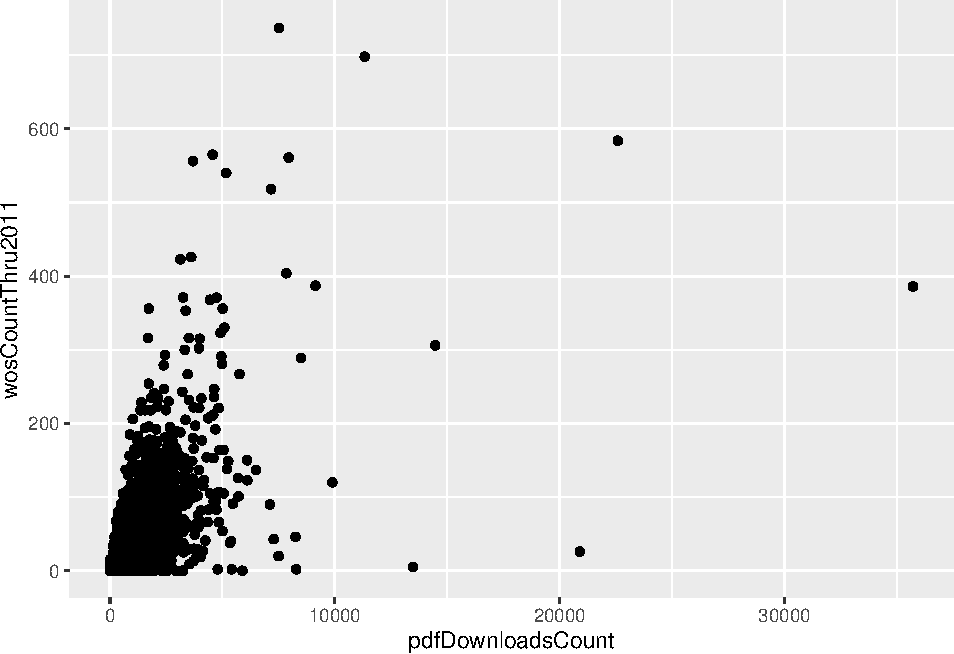
\includegraphics{Notes_files/figure-latex/unnamed-chunk-26-1.pdf}

Adding aesthetics:

\begin{Shaded}
\begin{Highlighting}[]
\NormalTok{p <-}\StringTok{ }\KeywordTok{ggplot}\NormalTok{(research, }\KeywordTok{aes}\NormalTok{(}\DataTypeTok{x =}\NormalTok{ pdfDownloadsCount,}
                          \DataTypeTok{y =}\NormalTok{ wosCountThru2011)) }\OperatorTok{+}
\StringTok{  }\KeywordTok{geom_point}\NormalTok{(}\KeywordTok{aes}\NormalTok{(}\DataTypeTok{color =}\NormalTok{ journal))}
\NormalTok{p}
\end{Highlighting}
\end{Shaded}

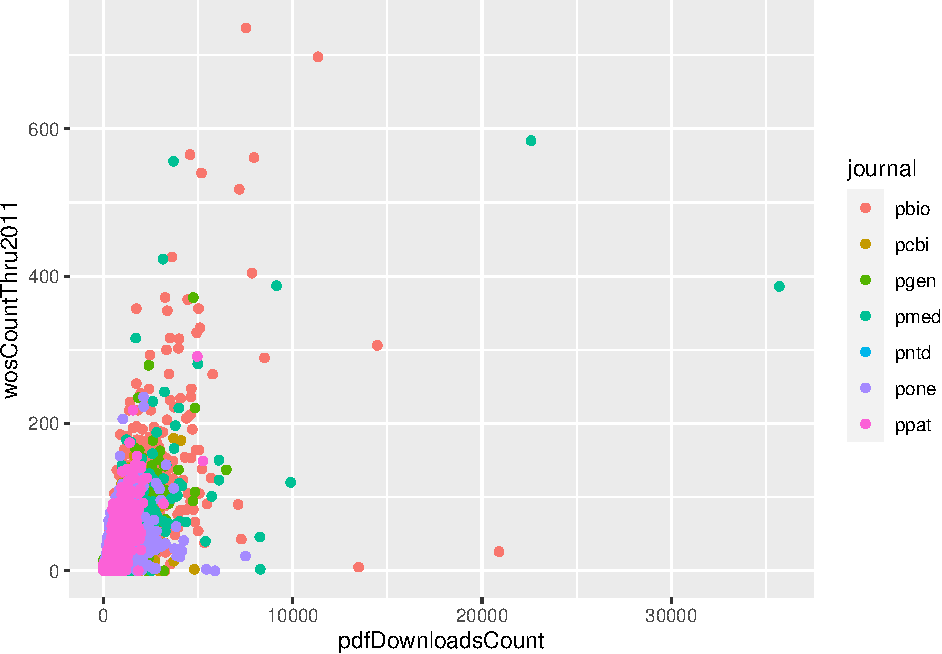
\includegraphics{Notes_files/figure-latex/unnamed-chunk-27-1.pdf}

\hypertarget{statistics}{%
\section{Statistics}\label{statistics}}

The function \texttt{geom\_smooth()} adds a loess curve to the data along with a 95\% confidence interval.

\begin{Shaded}
\begin{Highlighting}[]
\NormalTok{p <-}\StringTok{ }\KeywordTok{ggplot}\NormalTok{(research, }\KeywordTok{aes}\NormalTok{(}\DataTypeTok{x =}\NormalTok{ pdfDownloadsCount,}
                          \DataTypeTok{y =}\NormalTok{ wosCountThru2011)) }\OperatorTok{+}
\StringTok{  }\KeywordTok{geom_point}\NormalTok{(}\KeywordTok{aes}\NormalTok{(}\DataTypeTok{color =}\NormalTok{ journal)) }\OperatorTok{+}
\StringTok{  }\KeywordTok{geom_smooth}\NormalTok{()}
\NormalTok{p}
\end{Highlighting}
\end{Shaded}

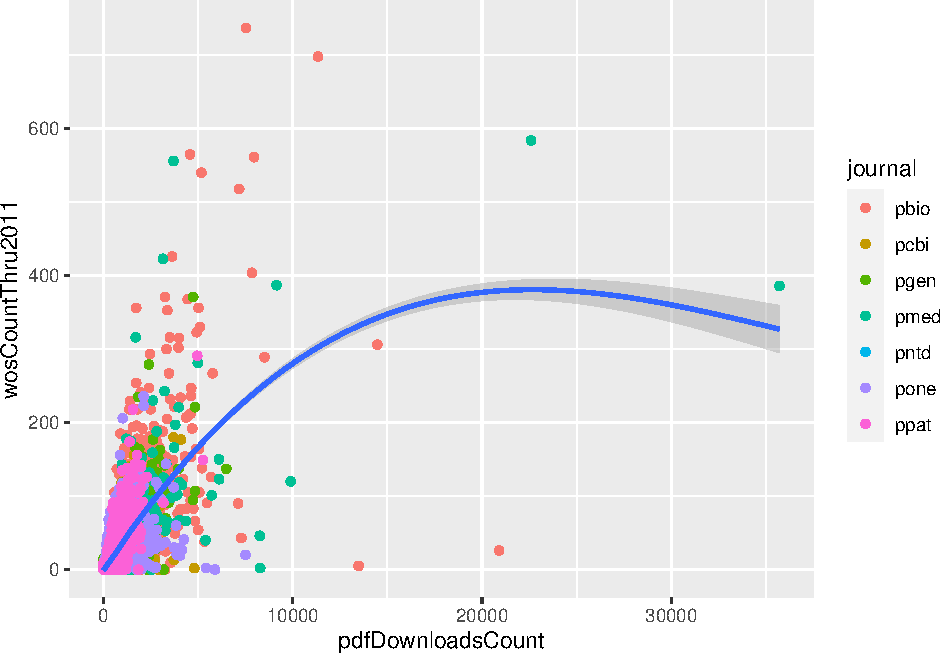
\includegraphics{Notes_files/figure-latex/unnamed-chunk-28-1.pdf}

If we move the colour to the base ggplot call, we get loess curves for each level of that factor.

\begin{Shaded}
\begin{Highlighting}[]
\NormalTok{p <-}\StringTok{ }\KeywordTok{ggplot}\NormalTok{(research, }\KeywordTok{aes}\NormalTok{(}\DataTypeTok{x =}\NormalTok{ pdfDownloadsCount, }
                          \DataTypeTok{y =}\NormalTok{ wosCountThru2011, }
                          \DataTypeTok{color =}\NormalTok{ journal)) }\OperatorTok{+}\StringTok{ }
\StringTok{  }\KeywordTok{geom_point}\NormalTok{() }\OperatorTok{+}\StringTok{ }
\StringTok{  }\KeywordTok{geom_smooth}\NormalTok{()}
\NormalTok{p}
\end{Highlighting}
\end{Shaded}

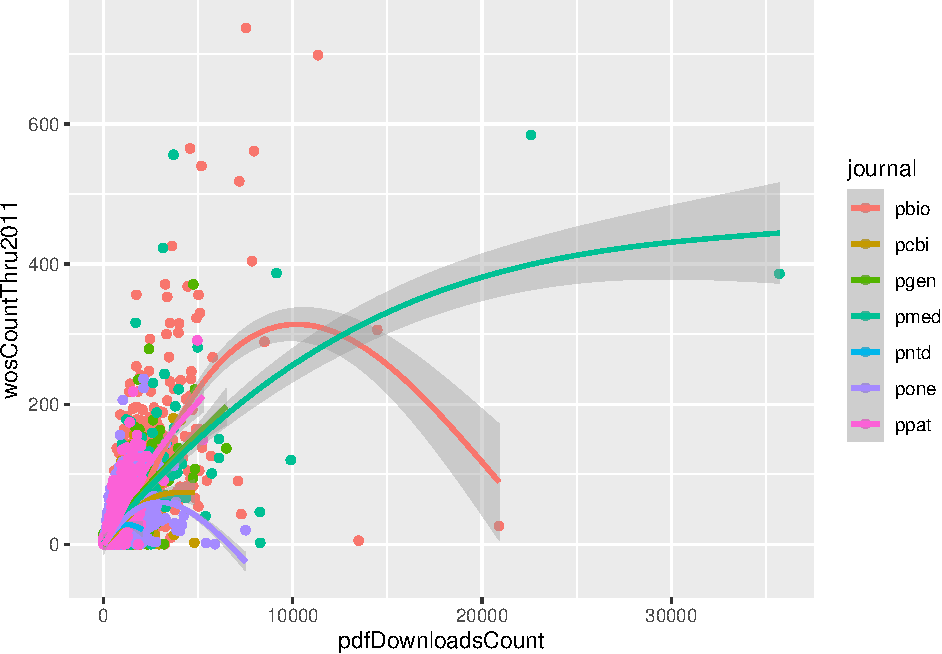
\includegraphics{Notes_files/figure-latex/unnamed-chunk-29-1.pdf}

Check the help page for the function \texttt{geom\_smooth()} for more information about how the curve is made. For example, to map a linear model onto the plot, you can choose \texttt{method\ =\ "lm"}.

\begin{Shaded}
\begin{Highlighting}[]
\NormalTok{p <-}\StringTok{ }\KeywordTok{ggplot}\NormalTok{(research, }\KeywordTok{aes}\NormalTok{(}\DataTypeTok{x =}\NormalTok{ pdfDownloadsCount, }
                          \DataTypeTok{y =}\NormalTok{ wosCountThru2011, }
                          \DataTypeTok{color =}\NormalTok{ journal)) }\OperatorTok{+}\StringTok{ }
\StringTok{  }\KeywordTok{geom_point}\NormalTok{() }\OperatorTok{+}\StringTok{ }
\StringTok{  }\KeywordTok{geom_smooth}\NormalTok{(}\DataTypeTok{method =} \StringTok{"lm"}\NormalTok{)}
\NormalTok{p}
\end{Highlighting}
\end{Shaded}

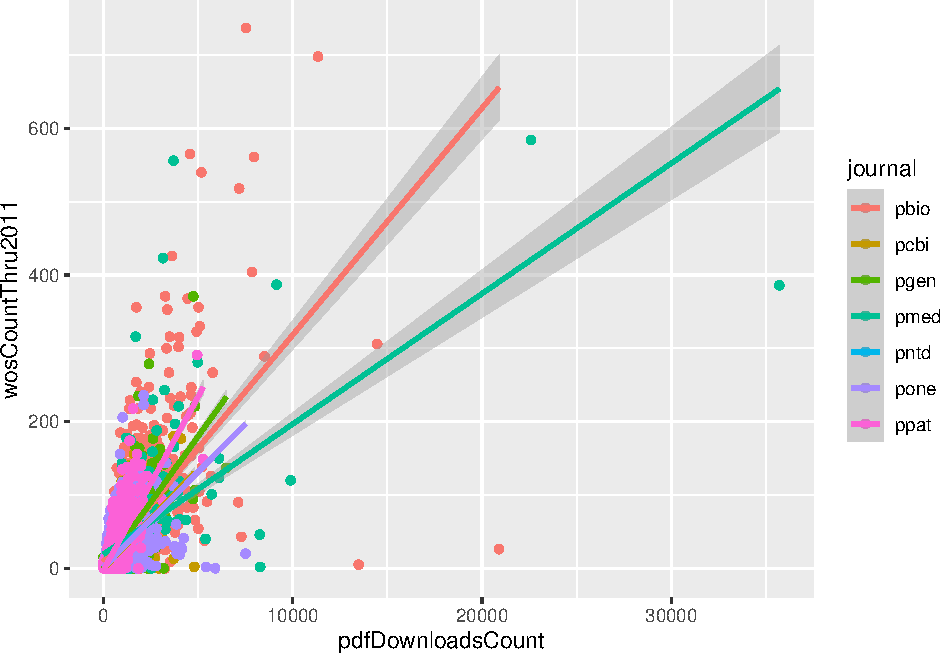
\includegraphics{Notes_files/figure-latex/unnamed-chunk-30-1.pdf}

\hypertarget{scales}{%
\section{Scales}\label{scales}}

Now let's look at the relationship between days since published and citation count.

\begin{Shaded}
\begin{Highlighting}[]
\NormalTok{p <-}\StringTok{ }\KeywordTok{ggplot}\NormalTok{(research, }\KeywordTok{aes}\NormalTok{(}\DataTypeTok{x =}\NormalTok{ daysSincePublished, }
                          \DataTypeTok{y =}\NormalTok{ wosCountThru2011)) }\OperatorTok{+}\StringTok{ }
\StringTok{  }\KeywordTok{geom_point}\NormalTok{(}\KeywordTok{aes}\NormalTok{(}\DataTypeTok{color=}\NormalTok{ journal))}
\NormalTok{p}
\end{Highlighting}
\end{Shaded}

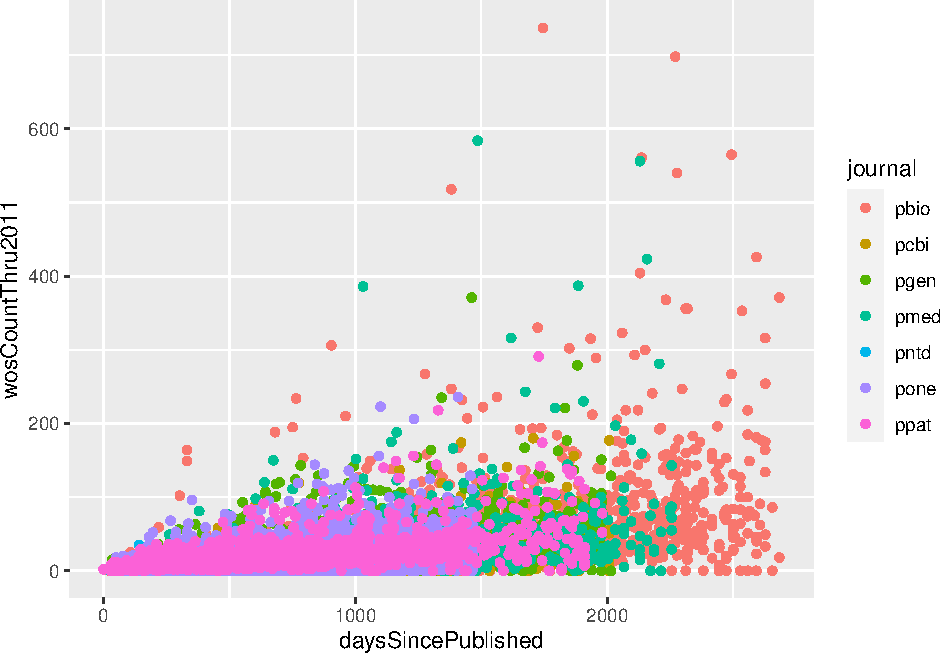
\includegraphics{Notes_files/figure-latex/unnamed-chunk-31-1.pdf}

It looks like most of the citation counts are close to 0. We can quickly check the distribution of this variable using a qplot.

\begin{Shaded}
\begin{Highlighting}[]
\KeywordTok{qplot}\NormalTok{(}\DataTypeTok{data =}\NormalTok{ research, }\DataTypeTok{x =}\NormalTok{ wosCountThru2011)}
\end{Highlighting}
\end{Shaded}

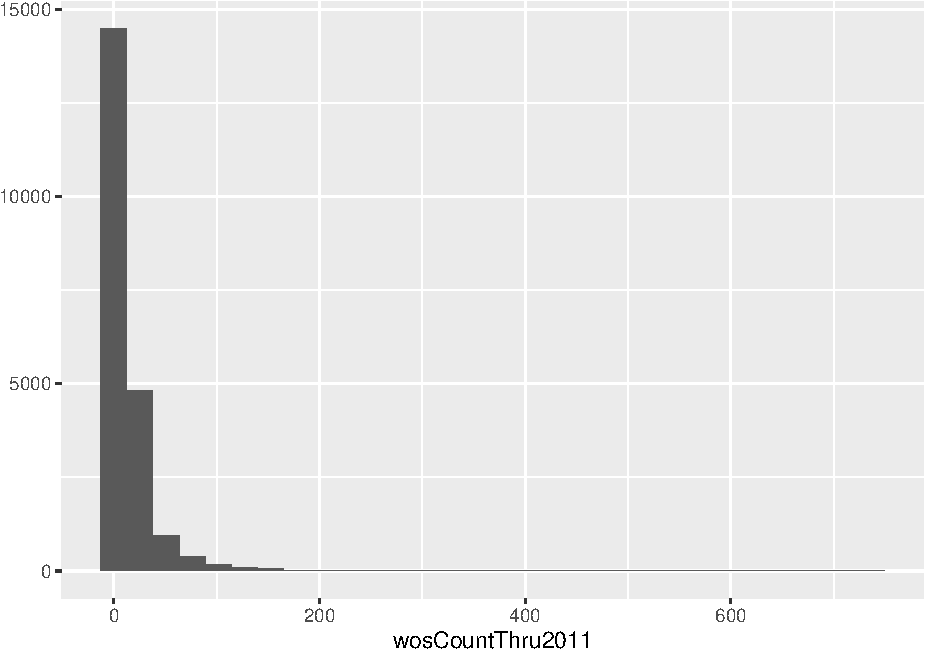
\includegraphics{Notes_files/figure-latex/unnamed-chunk-32-1.pdf}

To control the plot axes, we use variants of the functions \texttt{scale\_x\_*} and \texttt{scale\_y\_*}.

\begin{Shaded}
\begin{Highlighting}[]
\NormalTok{p <-}\StringTok{ }\KeywordTok{ggplot}\NormalTok{(research, }\KeywordTok{aes}\NormalTok{(}\DataTypeTok{x =}\NormalTok{ daysSincePublished, }
                          \DataTypeTok{y =}\NormalTok{ wosCountThru2011)) }\OperatorTok{+}\StringTok{ }
\StringTok{  }\KeywordTok{geom_point}\NormalTok{(}\KeywordTok{aes}\NormalTok{(}\DataTypeTok{color=}\NormalTok{ journal)) }\OperatorTok{+}
\StringTok{  }\KeywordTok{scale_y_log10}\NormalTok{()}
\NormalTok{p}
\end{Highlighting}
\end{Shaded}

\begin{verbatim}
## Warning: Transformation introduced infinite values in continuous y-axis
\end{verbatim}

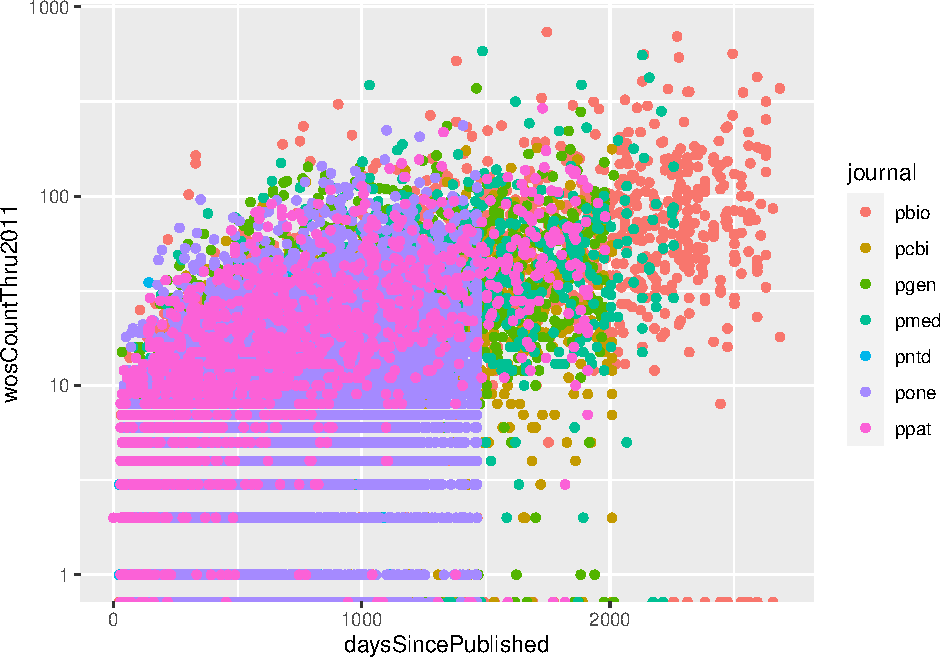
\includegraphics{Notes_files/figure-latex/unnamed-chunk-33-1.pdf}

How can we fix this?

\begin{Shaded}
\begin{Highlighting}[]
\NormalTok{p <-}\StringTok{ }\KeywordTok{ggplot}\NormalTok{(research, }\KeywordTok{aes}\NormalTok{(}\DataTypeTok{x =}\NormalTok{ daysSincePublished, }
                          \DataTypeTok{y =} \KeywordTok{log10}\NormalTok{(wosCountThru2011 }\OperatorTok{+}\StringTok{ }\DecValTok{1}\NormalTok{))) }\OperatorTok{+}\StringTok{ }
\StringTok{  }\KeywordTok{geom_point}\NormalTok{(}\KeywordTok{aes}\NormalTok{(}\DataTypeTok{color=}\NormalTok{ journal))}
\NormalTok{p}
\end{Highlighting}
\end{Shaded}

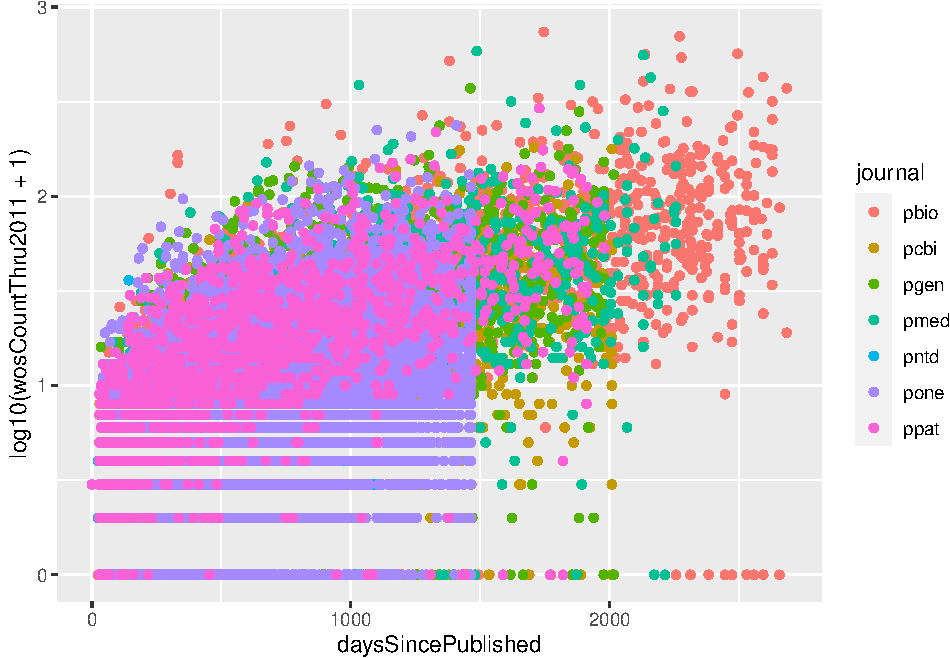
\includegraphics{Notes_files/figure-latex/unnamed-chunk-34-1.pdf}

Notice what this fix has done to the way the y-axis is labelled. To manually update the axis label, we can use the \texttt{scale\_y\_continuous()} function.

\begin{Shaded}
\begin{Highlighting}[]
\NormalTok{p <-}\StringTok{ }\KeywordTok{ggplot}\NormalTok{(research, }\KeywordTok{aes}\NormalTok{(}\DataTypeTok{x =}\NormalTok{ daysSincePublished, }
                          \DataTypeTok{y =} \KeywordTok{log10}\NormalTok{(wosCountThru2011 }\OperatorTok{+}\StringTok{ }\DecValTok{1}\NormalTok{))) }\OperatorTok{+}\StringTok{ }
\StringTok{  }\KeywordTok{geom_point}\NormalTok{(}\KeywordTok{aes}\NormalTok{(}\DataTypeTok{color=}\NormalTok{ journal)) }\OperatorTok{+}
\StringTok{  }\KeywordTok{scale_y_continuous}\NormalTok{(}\DataTypeTok{breaks =} \KeywordTok{c}\NormalTok{(}\DecValTok{1}\NormalTok{,}\DecValTok{2}\NormalTok{,}\DecValTok{3}\NormalTok{), }\DataTypeTok{labels =} \KeywordTok{c}\NormalTok{(}\DecValTok{10}\NormalTok{, }\DecValTok{100}\NormalTok{, }\DecValTok{1000}\NormalTok{), }\DataTypeTok{name =} \StringTok{"Citations"}\NormalTok{)}
\NormalTok{p}
\end{Highlighting}
\end{Shaded}

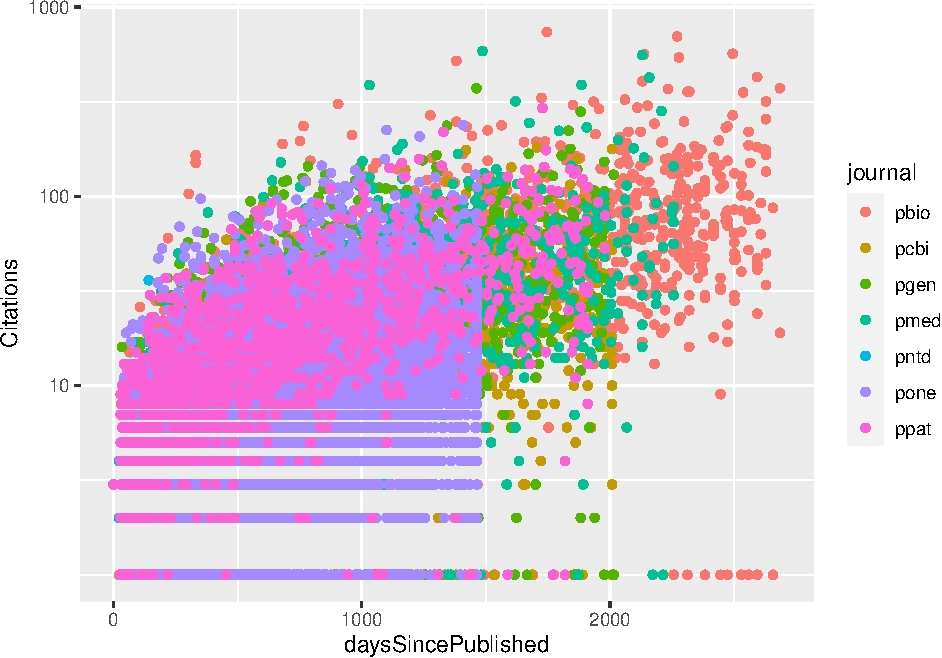
\includegraphics{Notes_files/figure-latex/unnamed-chunk-35-1.pdf}

The scale family of functions can also be used to change the colours.

\begin{Shaded}
\begin{Highlighting}[]
\NormalTok{p <-}\StringTok{ }\KeywordTok{ggplot}\NormalTok{(research, }\KeywordTok{aes}\NormalTok{(}\DataTypeTok{x =}\NormalTok{ daysSincePublished, }
                          \DataTypeTok{y =} \KeywordTok{log10}\NormalTok{(wosCountThru2011 }\OperatorTok{+}\StringTok{ }\DecValTok{1}\NormalTok{))) }\OperatorTok{+}\StringTok{ }
\StringTok{  }\KeywordTok{geom_point}\NormalTok{(}\KeywordTok{aes}\NormalTok{(}\DataTypeTok{color=}\NormalTok{ journal)) }\OperatorTok{+}
\StringTok{  }\KeywordTok{scale_y_continuous}\NormalTok{(}\DataTypeTok{breaks =} \KeywordTok{c}\NormalTok{(}\DecValTok{1}\NormalTok{,}\DecValTok{2}\NormalTok{,}\DecValTok{3}\NormalTok{), }\DataTypeTok{labels =} \KeywordTok{c}\NormalTok{(}\DecValTok{10}\NormalTok{, }\DecValTok{100}\NormalTok{,}\DecValTok{1000}\NormalTok{), }\DataTypeTok{name =} \StringTok{"Citations"}\NormalTok{) }\OperatorTok{+}
\StringTok{  }\KeywordTok{scale_colour_manual}\NormalTok{(}\DataTypeTok{values =} \KeywordTok{c}\NormalTok{(}\StringTok{"red"}\NormalTok{,}\StringTok{"blue"}\NormalTok{, }\StringTok{"green"}\NormalTok{, }\StringTok{"yellow"}\NormalTok{, }\StringTok{"purple"}\NormalTok{, }\StringTok{"orange"}\NormalTok{,}\StringTok{"cyan"}\NormalTok{), }\DataTypeTok{name =} \StringTok{"Journal"}\NormalTok{)}
\NormalTok{p}
\end{Highlighting}
\end{Shaded}

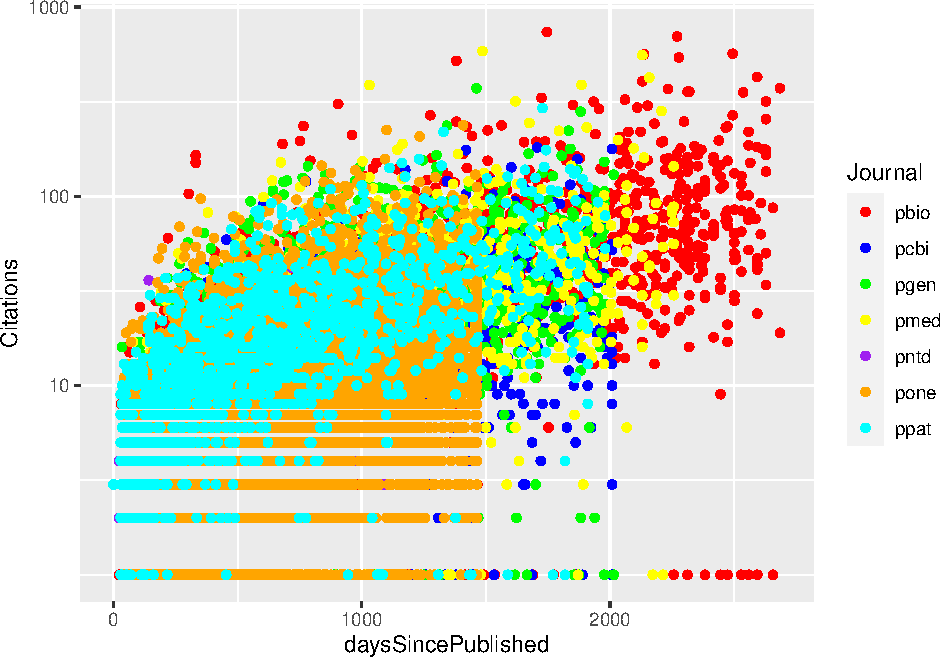
\includegraphics{Notes_files/figure-latex/unnamed-chunk-36-1.pdf}

\begin{Shaded}
\begin{Highlighting}[]
\KeywordTok{library}\NormalTok{(viridis)}

\NormalTok{p <-}\StringTok{ }\KeywordTok{ggplot}\NormalTok{(research, }\KeywordTok{aes}\NormalTok{(}\DataTypeTok{x =}\NormalTok{ daysSincePublished, }
                          \DataTypeTok{y =} \KeywordTok{log10}\NormalTok{(wosCountThru2011 }\OperatorTok{+}\StringTok{ }\DecValTok{1}\NormalTok{))) }\OperatorTok{+}\StringTok{ }
\StringTok{  }\KeywordTok{geom_point}\NormalTok{(}\KeywordTok{aes}\NormalTok{(}\DataTypeTok{color=}\NormalTok{ journal)) }\OperatorTok{+}
\StringTok{  }\KeywordTok{scale_y_continuous}\NormalTok{(}\DataTypeTok{breaks =} \KeywordTok{c}\NormalTok{(}\DecValTok{1}\NormalTok{,}\DecValTok{2}\NormalTok{,}\DecValTok{3}\NormalTok{), }\DataTypeTok{labels =} \KeywordTok{c}\NormalTok{(}\DecValTok{10}\NormalTok{, }\DecValTok{100}\NormalTok{,}\DecValTok{1000}\NormalTok{), }\DataTypeTok{name =} \StringTok{"Citations"}\NormalTok{) }\OperatorTok{+}
\StringTok{  }\KeywordTok{scale_colour_manual}\NormalTok{(}\DataTypeTok{values =} \KeywordTok{viridis}\NormalTok{(}\DecValTok{7}\NormalTok{), }\DataTypeTok{name =} \StringTok{"Journal"}\NormalTok{)}
\NormalTok{p}
\end{Highlighting}
\end{Shaded}

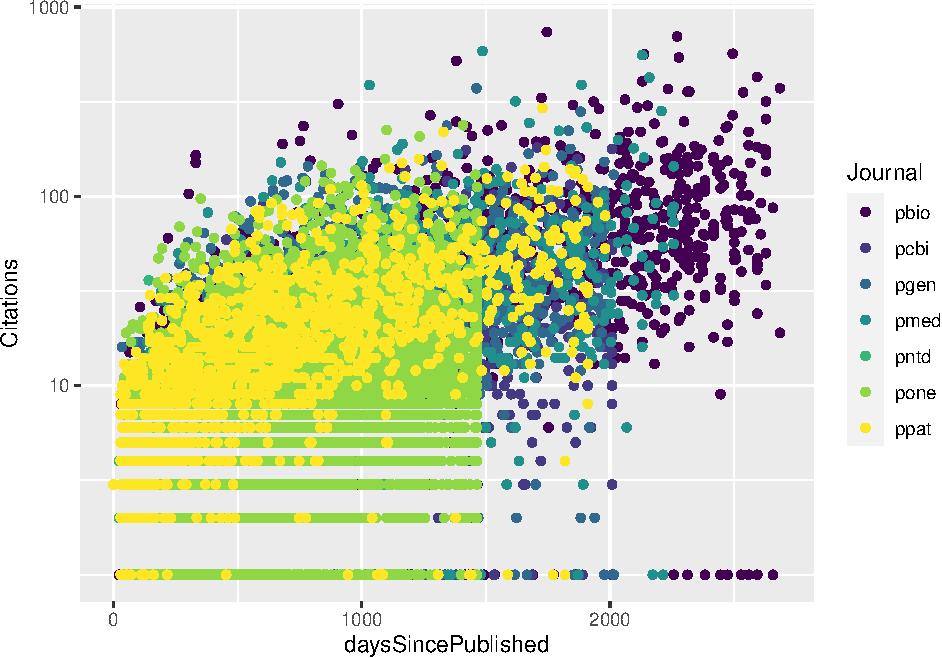
\includegraphics{Notes_files/figure-latex/unnamed-chunk-36-2.pdf}

\hypertarget{colour-palettes}{%
\section{Colour palettes}\label{colour-palettes}}

Choosing good colours to aid visualization is not trivial and requires some (or a lot of) thought. A set of colour palettes have been developed for easy use with ggplot2 through a package called \texttt{RColorBrewer}.

There are three types of these premade palettes:
* Sequential
* Diverging
* Qualitative

\begin{Shaded}
\begin{Highlighting}[]
\KeywordTok{library}\NormalTok{(RColorBrewer)}
\KeywordTok{display.brewer.all}\NormalTok{()}
\end{Highlighting}
\end{Shaded}

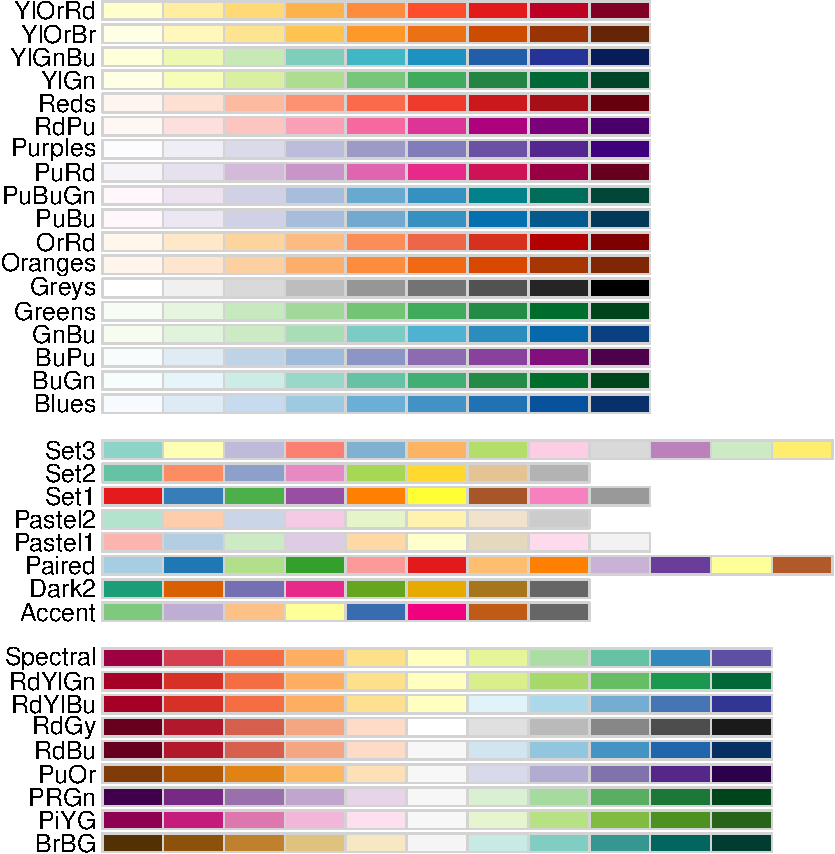
\includegraphics{Notes_files/figure-latex/unnamed-chunk-37-1.pdf}

Or, you can create your own color palettes using the \texttt{colorRamp()} or \texttt{colorRampPalette()} function.

\texttt{colorRamp()} returns a function that takes values between 0 and 1, indicating the extremes of the color palette.

\texttt{colorRampPalette()} returns a function that takes integer arguments and returns a vector of colours.

\hypertarget{colorramp}{%
\subsection*{\texorpdfstring{\texttt{colorRamp()}}{colorRamp()}}\label{colorramp}}
\addcontentsline{toc}{subsection}{\texttt{colorRamp()}}

\begin{Shaded}
\begin{Highlighting}[]
\NormalTok{cols <-}\StringTok{ }\KeywordTok{colorRamp}\NormalTok{(}\KeywordTok{c}\NormalTok{(}\StringTok{"red"}\NormalTok{, }\StringTok{"blue"}\NormalTok{))}
\KeywordTok{cols}\NormalTok{(}\DecValTok{0}\NormalTok{)}
\end{Highlighting}
\end{Shaded}

\begin{verbatim}
##      [,1] [,2] [,3]
## [1,]  255    0    0
\end{verbatim}

\begin{Shaded}
\begin{Highlighting}[]
\KeywordTok{cols}\NormalTok{(}\FloatTok{0.5}\NormalTok{)}
\end{Highlighting}
\end{Shaded}

\begin{verbatim}
##       [,1] [,2]  [,3]
## [1,] 127.5    0 127.5
\end{verbatim}

\begin{Shaded}
\begin{Highlighting}[]
\KeywordTok{cols}\NormalTok{(}\DecValTok{1}\NormalTok{)}
\end{Highlighting}
\end{Shaded}

\begin{verbatim}
##      [,1] [,2] [,3]
## [1,]    0    0  255
\end{verbatim}

\hypertarget{colorramppalette}{%
\subsection*{\texorpdfstring{\texttt{colorRampPalette()}}{colorRampPalette()}}\label{colorramppalette}}
\addcontentsline{toc}{subsection}{\texttt{colorRampPalette()}}

\begin{Shaded}
\begin{Highlighting}[]
\NormalTok{cols <-}\StringTok{ }\KeywordTok{colorRampPalette}\NormalTok{(}\KeywordTok{c}\NormalTok{(}\StringTok{"red"}\NormalTok{, }\StringTok{"blue"}\NormalTok{))}
\KeywordTok{cols}\NormalTok{(}\DecValTok{2}\NormalTok{)}
\end{Highlighting}
\end{Shaded}

\begin{verbatim}
## [1] "#FF0000" "#0000FF"
\end{verbatim}

\begin{Shaded}
\begin{Highlighting}[]
\KeywordTok{cols}\NormalTok{(}\DecValTok{10}\NormalTok{)}
\end{Highlighting}
\end{Shaded}

\begin{verbatim}
##  [1] "#FF0000" "#E2001C" "#C60038" "#AA0055" "#8D0071" "#71008D" "#5500AA"
##  [8] "#3800C6" "#1C00E2" "#0000FF"
\end{verbatim}

\hypertarget{faceting}{%
\section{Faceting}\label{faceting}}

There are two functions to control how plots are divided into facets: \texttt{facet\_wrap()} and \texttt{facet\_grid()}.

\hypertarget{facet_wrap}{%
\subsection*{\texorpdfstring{\texttt{facet\_wrap()}}{facet\_wrap()}}\label{facet_wrap}}
\addcontentsline{toc}{subsection}{\texttt{facet\_wrap()}}

\begin{Shaded}
\begin{Highlighting}[]
\NormalTok{p <-}\StringTok{ }\KeywordTok{ggplot}\NormalTok{(research, }\KeywordTok{aes}\NormalTok{(}\DataTypeTok{x =}\NormalTok{ daysSincePublished, }
                          \DataTypeTok{y =} \KeywordTok{log10}\NormalTok{(wosCountThru2011 }\OperatorTok{+}\StringTok{ }\DecValTok{1}\NormalTok{),}
                          \DataTypeTok{color =}\NormalTok{ journal)) }\OperatorTok{+}
\StringTok{  }\KeywordTok{geom_point}\NormalTok{() }\OperatorTok{+}
\StringTok{  }\KeywordTok{scale_y_continuous}\NormalTok{(}\DataTypeTok{breaks =} \KeywordTok{c}\NormalTok{(}\DecValTok{1}\NormalTok{,}\DecValTok{2}\NormalTok{,}\DecValTok{3}\NormalTok{), }\DataTypeTok{labels =} \KeywordTok{c}\NormalTok{(}\DecValTok{10}\NormalTok{, }\DecValTok{100}\NormalTok{,}\DecValTok{1000}\NormalTok{), }\DataTypeTok{name =} \StringTok{"Citations"}\NormalTok{) }\OperatorTok{+}
\StringTok{  }\KeywordTok{facet_wrap}\NormalTok{(}\OperatorTok{~}\NormalTok{journal) }\OperatorTok{+}
\StringTok{  }\KeywordTok{geom_smooth}\NormalTok{(}\DataTypeTok{color =} \StringTok{"black"}\NormalTok{, }\DataTypeTok{method =} \StringTok{"lm"}\NormalTok{)}
\NormalTok{p}
\end{Highlighting}
\end{Shaded}

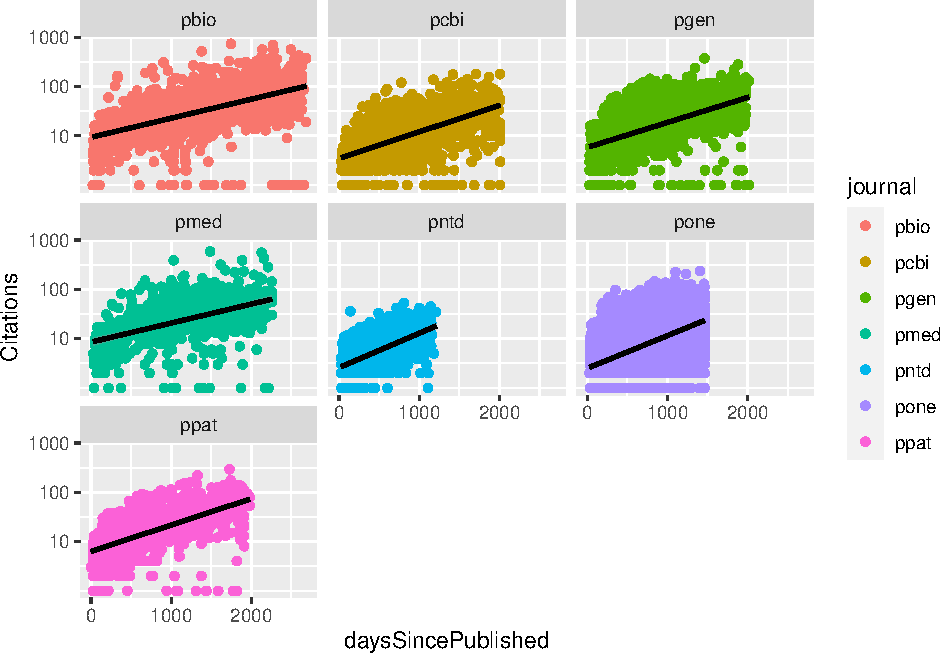
\includegraphics{Notes_files/figure-latex/unnamed-chunk-40-1.pdf}

It is still difficult to see the spread of the data. Try making the points smaller and transparent.

\begin{Shaded}
\begin{Highlighting}[]
\NormalTok{p <-}\StringTok{ }\KeywordTok{ggplot}\NormalTok{(research, }\KeywordTok{aes}\NormalTok{(}\DataTypeTok{x =}\NormalTok{ daysSincePublished, }
                          \DataTypeTok{y =} \KeywordTok{log10}\NormalTok{(wosCountThru2011 }\OperatorTok{+}\StringTok{ }\DecValTok{1}\NormalTok{),}
                          \DataTypeTok{color =}\NormalTok{ journal)) }\OperatorTok{+}
\StringTok{  }\KeywordTok{geom_point}\NormalTok{(}\DataTypeTok{size =} \FloatTok{0.5}\NormalTok{, }\DataTypeTok{alpha =} \FloatTok{0.5}\NormalTok{) }\OperatorTok{+}
\StringTok{  }\KeywordTok{scale_y_continuous}\NormalTok{(}\DataTypeTok{breaks =} \KeywordTok{c}\NormalTok{(}\DecValTok{1}\NormalTok{,}\DecValTok{2}\NormalTok{,}\DecValTok{3}\NormalTok{), }\DataTypeTok{labels =} \KeywordTok{c}\NormalTok{(}\DecValTok{10}\NormalTok{, }\DecValTok{100}\NormalTok{,}\DecValTok{1000}\NormalTok{), }\DataTypeTok{name =} \StringTok{"Citations"}\NormalTok{) }\OperatorTok{+}
\StringTok{  }\KeywordTok{facet_wrap}\NormalTok{(}\OperatorTok{~}\NormalTok{journal) }\OperatorTok{+}
\StringTok{  }\KeywordTok{geom_smooth}\NormalTok{(}\DataTypeTok{color =} \StringTok{"black"}\NormalTok{, }\DataTypeTok{method =} \StringTok{"lm"}\NormalTok{)}
\NormalTok{p}
\end{Highlighting}
\end{Shaded}

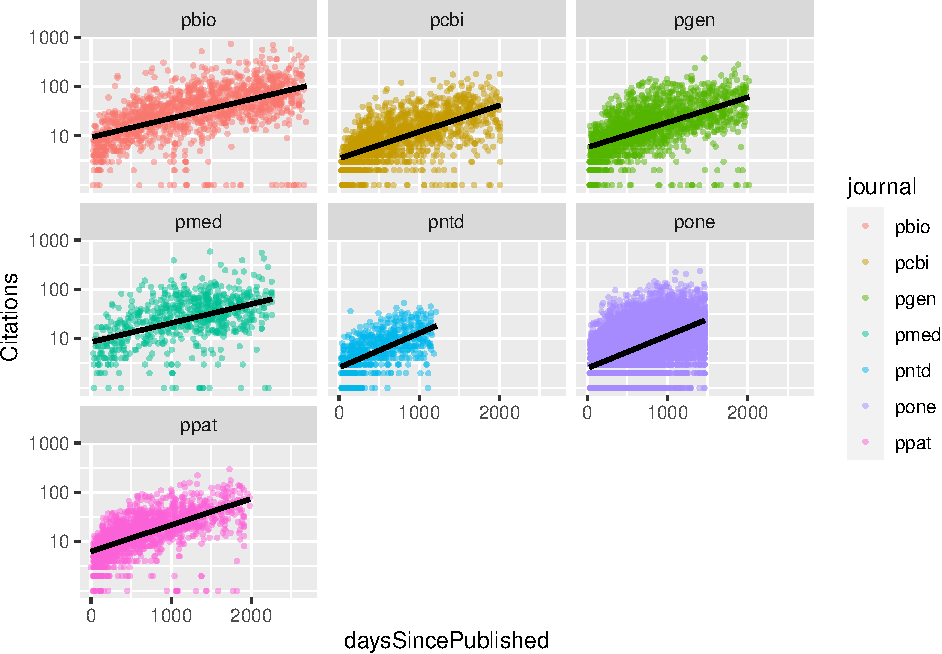
\includegraphics{Notes_files/figure-latex/unnamed-chunk-41-1.pdf}

\hypertarget{facet_grid}{%
\subsection*{\texorpdfstring{\texttt{facet\_grid()}}{facet\_grid()}}\label{facet_grid}}
\addcontentsline{toc}{subsection}{\texttt{facet\_grid()}}

What about faceting by two variables? For example, let's say we want to look at the relationship between days since published and citations for low impact versus high impact articles.

First, let's recreate a variable categorizing high and low impact based on the variable \texttt{f1000Factor}.

\begin{Shaded}
\begin{Highlighting}[]
\NormalTok{research <-}\StringTok{ }\NormalTok{research }\OperatorTok\StringTok{ }\KeywordTok{mutate}\NormalTok{(}\DataTypeTok{impact =} \KeywordTok{cut}\NormalTok{(f1000Factor, }\DataTypeTok{breaks =} \KeywordTok{c}\NormalTok{(}\OperatorTok{-}\OtherTok{Inf}\NormalTok{,}\DecValTok{1}\NormalTok{,}\OtherTok{Inf}\NormalTok{), }\DataTypeTok{labels =} \KeywordTok{c}\NormalTok{(}\StringTok{"low"}\NormalTok{, }\StringTok{"high"}\NormalTok{)))}

\NormalTok{p <-}\StringTok{ }\KeywordTok{ggplot}\NormalTok{(research, }\KeywordTok{aes}\NormalTok{(}\DataTypeTok{x =}\NormalTok{ daysSincePublished, }
                          \DataTypeTok{y =} \KeywordTok{log10}\NormalTok{(wosCountThru2011 }\OperatorTok{+}\StringTok{ }\DecValTok{1}\NormalTok{),}
                          \DataTypeTok{color =}\NormalTok{ journal)) }\OperatorTok{+}
\StringTok{  }\KeywordTok{geom_point}\NormalTok{(}\DataTypeTok{size =} \FloatTok{0.5}\NormalTok{, }\DataTypeTok{alpha =} \FloatTok{0.5}\NormalTok{) }\OperatorTok{+}
\StringTok{  }\KeywordTok{scale_y_continuous}\NormalTok{(}\DataTypeTok{breaks =} \KeywordTok{c}\NormalTok{(}\DecValTok{1}\NormalTok{,}\DecValTok{2}\NormalTok{,}\DecValTok{3}\NormalTok{), }\DataTypeTok{labels =} \KeywordTok{c}\NormalTok{(}\DecValTok{10}\NormalTok{, }\DecValTok{100}\NormalTok{,}\DecValTok{1000}\NormalTok{), }\DataTypeTok{name =} \StringTok{"Citations"}\NormalTok{) }\OperatorTok{+}
\StringTok{  }\KeywordTok{facet_grid}\NormalTok{(journal}\OperatorTok{~}\NormalTok{impact) }\OperatorTok{+}
\StringTok{  }\KeywordTok{geom_smooth}\NormalTok{(}\DataTypeTok{color =} \StringTok{"black"}\NormalTok{, }\DataTypeTok{method =} \StringTok{"lm"}\NormalTok{)}
\NormalTok{p}
\end{Highlighting}
\end{Shaded}

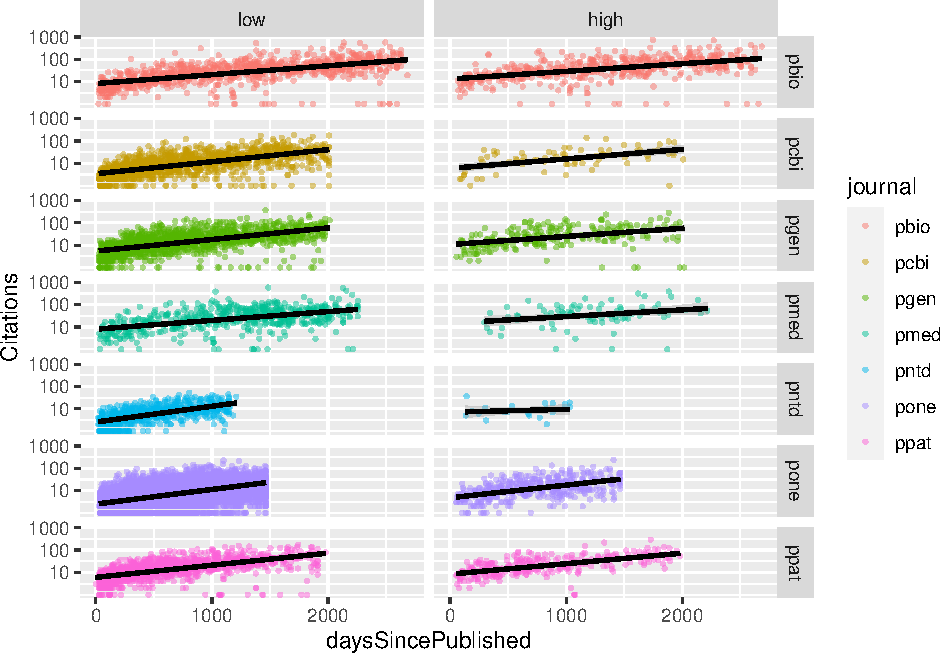
\includegraphics{Notes_files/figure-latex/unnamed-chunk-42-1.pdf}

By default, R will plot each panel on the same axes. You can override this using the option \texttt{scales}, setting it to \texttt{free\_x} to vary the scale across rows, \texttt{scale\_y} to vary it across columns, or \texttt{free} to vary across both.

\begin{Shaded}
\begin{Highlighting}[]
\NormalTok{p <-}\StringTok{ }\KeywordTok{ggplot}\NormalTok{(research, }\KeywordTok{aes}\NormalTok{(}\DataTypeTok{x =}\NormalTok{ daysSincePublished, }
                          \DataTypeTok{y =} \KeywordTok{log10}\NormalTok{(wosCountThru2011 }\OperatorTok{+}\StringTok{ }\DecValTok{1}\NormalTok{),}
                          \DataTypeTok{color =}\NormalTok{ journal)) }\OperatorTok{+}
\StringTok{  }\KeywordTok{geom_point}\NormalTok{(}\DataTypeTok{size =} \FloatTok{0.5}\NormalTok{, }\DataTypeTok{alpha =} \FloatTok{0.5}\NormalTok{) }\OperatorTok{+}
\StringTok{  }\KeywordTok{scale_y_continuous}\NormalTok{(}\DataTypeTok{breaks =} \KeywordTok{c}\NormalTok{(}\DecValTok{1}\NormalTok{,}\DecValTok{2}\NormalTok{,}\DecValTok{3}\NormalTok{), }\DataTypeTok{labels =} \KeywordTok{c}\NormalTok{(}\DecValTok{10}\NormalTok{, }\DecValTok{100}\NormalTok{,}\DecValTok{1000}\NormalTok{), }\DataTypeTok{name =} \StringTok{"Citations"}\NormalTok{) }\OperatorTok{+}
\StringTok{  }\KeywordTok{facet_wrap}\NormalTok{(}\OperatorTok{~}\NormalTok{journal, }\DataTypeTok{scale =} \StringTok{"free"}\NormalTok{) }\OperatorTok{+}
\StringTok{  }\KeywordTok{geom_smooth}\NormalTok{(}\DataTypeTok{color =} \StringTok{"black"}\NormalTok{, }\DataTypeTok{method =} \StringTok{"lm"}\NormalTok{)}
\NormalTok{p}
\end{Highlighting}
\end{Shaded}

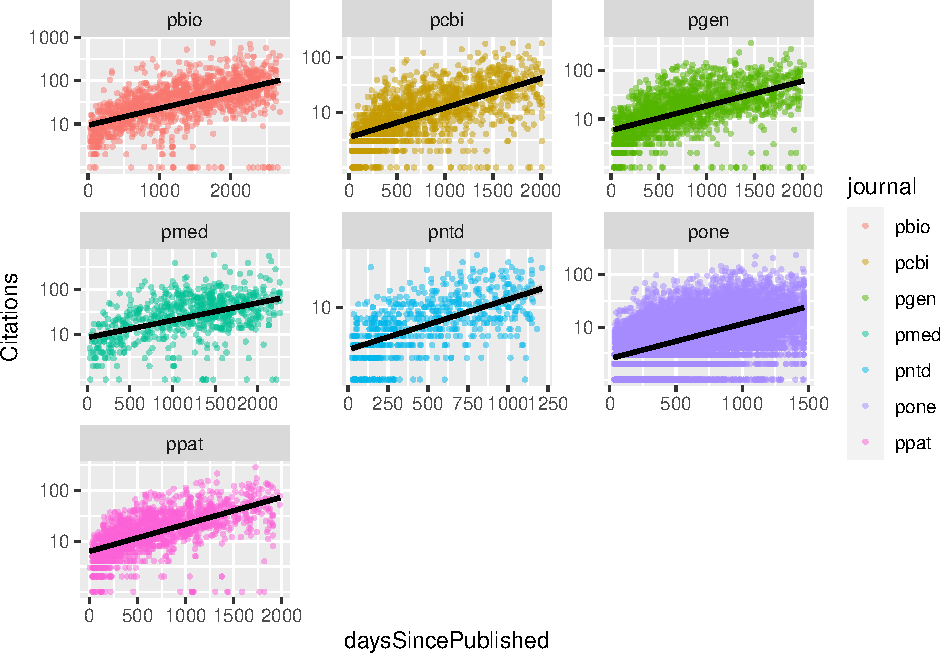
\includegraphics{Notes_files/figure-latex/unnamed-chunk-43-1.pdf}

\begin{center}\rule{0.5\linewidth}{0.5pt}\end{center}

\hypertarget{exercise-5.6}{%
\subsection*{Exercise 5.6}\label{exercise-5.6}}
\addcontentsline{toc}{subsection}{Exercise 5.6}

Use what you've learned to generate the plot below.

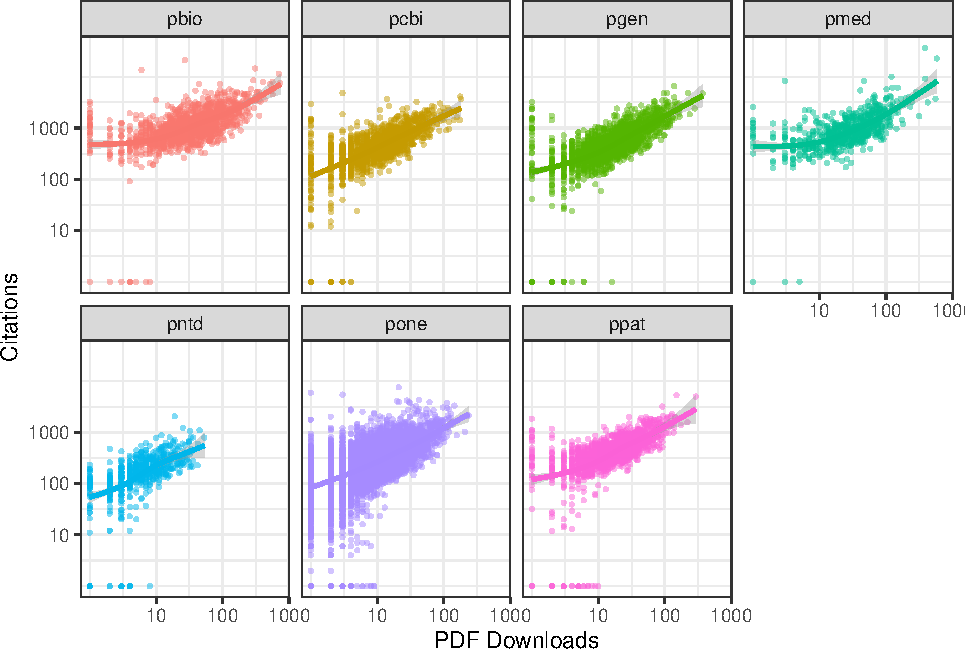
\includegraphics{Notes_files/figure-latex/unnamed-chunk-44-1.pdf}

\begin{center}\rule{0.5\linewidth}{0.5pt}\end{center}

\hypertarget{themes}{%
\section{Themes}\label{themes}}

In addition to \texttt{theme\_bw()}, which changes the plot background to white, \texttt{ggplot2} comes with several other themes which can be useful to quickly change the look of your visualization. The complete list of themes is available at \url{https://ggplot2.tidyverse.org/reference/ggtheme.html}. \texttt{theme\_minimal()} and \texttt{theme\_light()} are popular, and \texttt{theme\_void()} can be useful as a starting point to create a new hand-crafted theme.

The \texttt{ggthemes} package provides a wide variety of options (including an Excel 2003 theme). The \texttt{ggplot2} \href{https://www.ggplot2-exts.org}{extensions website} provides a list of packages that extend the capabilities of \texttt{ggplot2}, including additional themes.

This is also the place you can customize the text of your plot.

\begin{Shaded}
\begin{Highlighting}[]
\NormalTok{p <-}\StringTok{ }\KeywordTok{ggplot}\NormalTok{(research, }\KeywordTok{aes}\NormalTok{(}\DataTypeTok{x =}\NormalTok{ daysSincePublished, }
                          \DataTypeTok{y =} \KeywordTok{log10}\NormalTok{(wosCountThru2011 }\OperatorTok{+}\StringTok{ }\DecValTok{1}\NormalTok{))) }\OperatorTok{+}\StringTok{ }
\StringTok{  }\KeywordTok{geom_point}\NormalTok{(}\KeywordTok{aes}\NormalTok{(}\DataTypeTok{color=}\NormalTok{ journal)) }\OperatorTok{+}
\StringTok{  }\KeywordTok{scale_y_continuous}\NormalTok{(}\DataTypeTok{breaks =} \KeywordTok{c}\NormalTok{(}\DecValTok{1}\NormalTok{,}\DecValTok{2}\NormalTok{,}\DecValTok{3}\NormalTok{), }\DataTypeTok{labels =} \KeywordTok{c}\NormalTok{(}\DecValTok{10}\NormalTok{, }\DecValTok{100}\NormalTok{, }\DecValTok{1000}\NormalTok{), }\DataTypeTok{name =} \StringTok{"Citations"}\NormalTok{) }\OperatorTok{+}
\StringTok{  }\KeywordTok{theme_bw}\NormalTok{() }\OperatorTok{+}
\StringTok{  }\KeywordTok{xlab}\NormalTok{(}\StringTok{"Days Since Published"}\NormalTok{) }\OperatorTok{+}
\StringTok{  }\KeywordTok{theme}\NormalTok{(}\DataTypeTok{axis.title.x =} \KeywordTok{element_text}\NormalTok{(}\DataTypeTok{size =} \DecValTok{14}\NormalTok{, }\DataTypeTok{face =} \StringTok{"bold"}\NormalTok{))}
\NormalTok{p}
\end{Highlighting}
\end{Shaded}

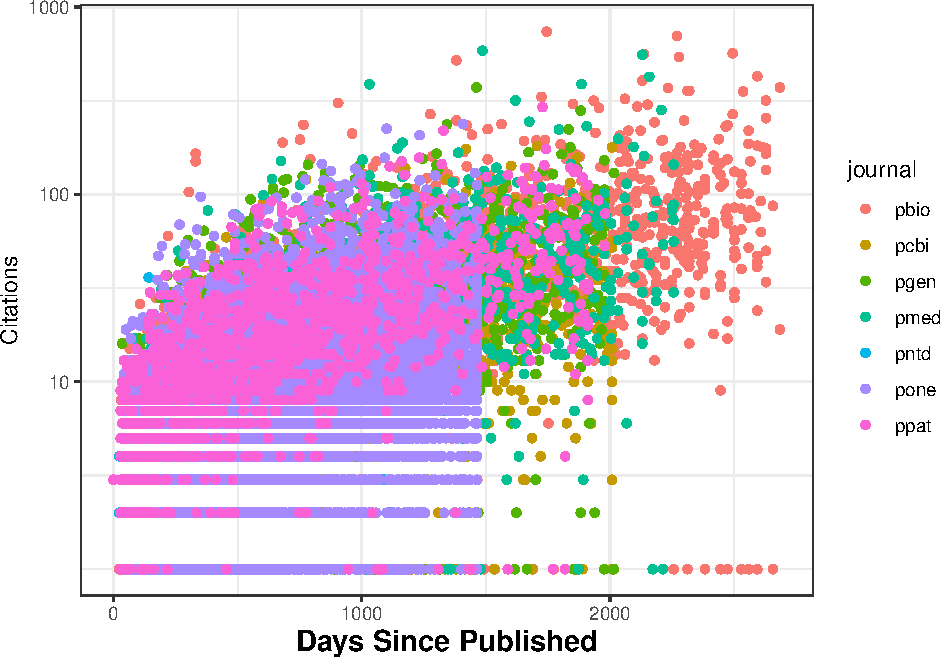
\includegraphics{Notes_files/figure-latex/unnamed-chunk-45-1.pdf}

\hypertarget{multiple-plots}{%
\section{Multiple plots}\label{multiple-plots}}

There are two useful packages for combining multiple plots: \texttt{gridExtra} and \texttt{cowplot}.

\texttt{gridExtra} has two useful functions: \texttt{grid.arrange()} and \texttt{arrangeGrob()}. However, these functions make no attempt at aligning the plot panels; instead, the plots are simply placed into the grid as they are, so the axes are not aligned. If axis alignment is required, the \texttt{plot\_grid()} function of the \texttt{cowplot} package is better. We will try using both here.

\hypertarget{the-gridextra-package}{%
\subsection*{\texorpdfstring{The \texttt{gridExtra} package}{The gridExtra package}}\label{the-gridextra-package}}
\addcontentsline{toc}{subsection}{The \texttt{gridExtra} package}

Let's say we want to combine the following three plots:

\begin{Shaded}
\begin{Highlighting}[]
\NormalTok{plot1 <-}\StringTok{ }\KeywordTok{ggplot}\NormalTok{(research, }\KeywordTok{aes}\NormalTok{(}\DataTypeTok{x =}\NormalTok{ journal, }\DataTypeTok{fill =}\NormalTok{ journal)) }\OperatorTok{+}
\StringTok{    }\KeywordTok{geom_bar}\NormalTok{(}\DataTypeTok{color =} \StringTok{"black"}\NormalTok{) }\OperatorTok{+}
\StringTok{    }\KeywordTok{theme_bw}\NormalTok{()}
\NormalTok{plot1}
\end{Highlighting}
\end{Shaded}

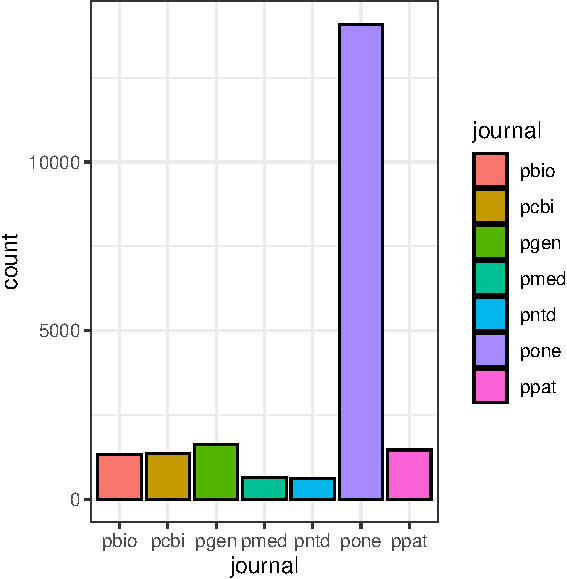
\includegraphics{Notes_files/figure-latex/unnamed-chunk-46-1.pdf}

\begin{Shaded}
\begin{Highlighting}[]
\NormalTok{plot2 <-}\StringTok{ }\KeywordTok{ggplot}\NormalTok{(research, }\KeywordTok{aes}\NormalTok{(}\DataTypeTok{x =} \KeywordTok{log10}\NormalTok{(wosCountThru2011 }\OperatorTok{+}\StringTok{ }\DecValTok{1}\NormalTok{),}
                              \DataTypeTok{y =} \KeywordTok{log10}\NormalTok{(pdfDownloadsCount }\OperatorTok{+}\StringTok{ }\DecValTok{1}\NormalTok{),}
                              \DataTypeTok{color =}\NormalTok{ journal)) }\OperatorTok{+}
\StringTok{    }\KeywordTok{geom_point}\NormalTok{(}\DataTypeTok{size =} \FloatTok{0.5}\NormalTok{, }\DataTypeTok{alpha =} \FloatTok{0.5}\NormalTok{) }\OperatorTok{+}
\StringTok{    }\KeywordTok{theme_bw}\NormalTok{() }\OperatorTok{+}
\StringTok{    }\KeywordTok{geom_smooth}\NormalTok{() }\OperatorTok{+}
\StringTok{  }\KeywordTok{xlab}\NormalTok{(}\StringTok{"Citations"}\NormalTok{) }\OperatorTok{+}
\StringTok{  }\KeywordTok{ylab}\NormalTok{(}\StringTok{"Downloads"}\NormalTok{) }\OperatorTok{+}
\StringTok{  }\KeywordTok{theme}\NormalTok{(}\DataTypeTok{legend.position =} \StringTok{"none"}\NormalTok{)}
\NormalTok{plot2}
\end{Highlighting}
\end{Shaded}

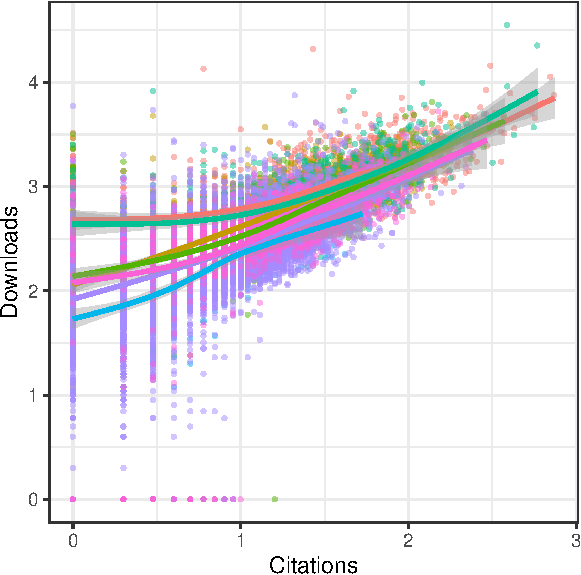
\includegraphics{Notes_files/figure-latex/unnamed-chunk-46-2.pdf}

\begin{Shaded}
\begin{Highlighting}[]
\NormalTok{plot3 <-}\StringTok{ }\KeywordTok{ggplot}\NormalTok{(research, }\KeywordTok{aes}\NormalTok{(}\DataTypeTok{x =}\NormalTok{ impact,}
                              \DataTypeTok{y =} \KeywordTok{log10}\NormalTok{(pdfDownloadsCount }\OperatorTok{+}\StringTok{ }\DecValTok{1}\NormalTok{),}
                              \DataTypeTok{fill =}\NormalTok{ journal)) }\OperatorTok{+}
\StringTok{    }\KeywordTok{geom_boxplot}\NormalTok{() }\OperatorTok{+}\StringTok{ }
\StringTok{    }\KeywordTok{theme_bw}\NormalTok{() }\OperatorTok{+}
\StringTok{  }\KeywordTok{ylab}\NormalTok{(}\StringTok{"Downloads"}\NormalTok{)}
\NormalTok{plot3}
\end{Highlighting}
\end{Shaded}

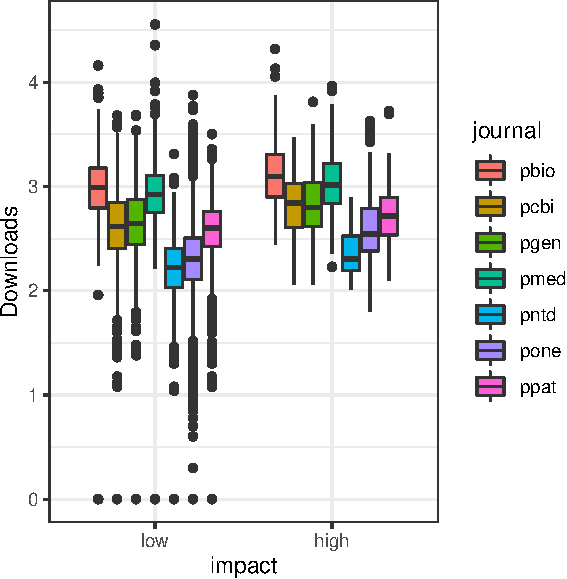
\includegraphics{Notes_files/figure-latex/unnamed-chunk-46-3.pdf}

To arrange them together, use the \texttt{grid.arrange()} function.

\begin{Shaded}
\begin{Highlighting}[]
\KeywordTok{library}\NormalTok{(gridExtra)}
\KeywordTok{grid.arrange}\NormalTok{(plot1, plot2, plot3)}
\end{Highlighting}
\end{Shaded}

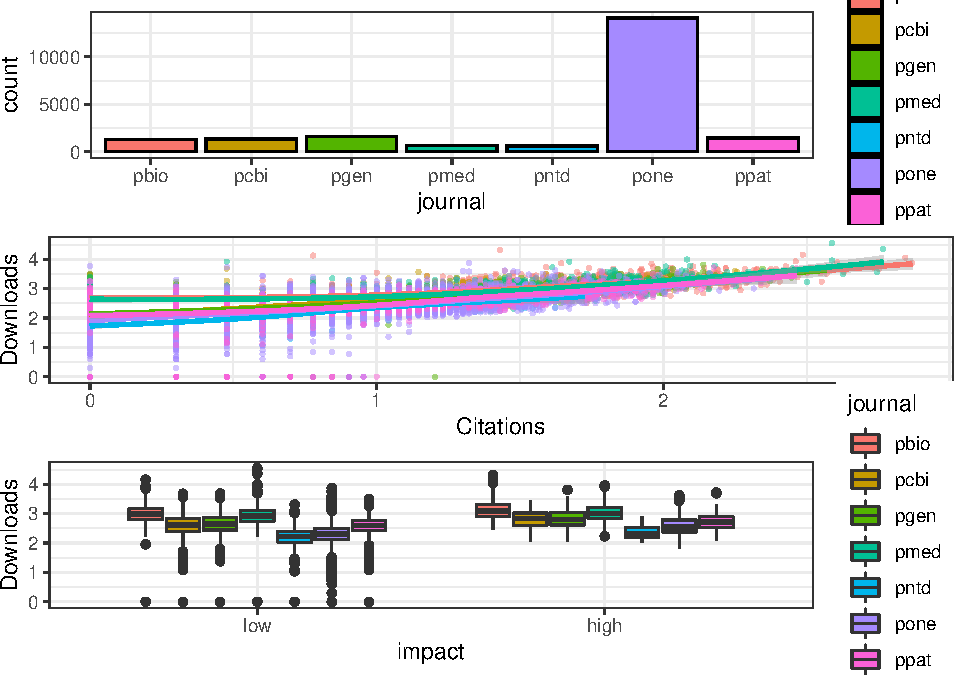
\includegraphics{Notes_files/figure-latex/unnamed-chunk-47-1.pdf}

To modify how they are arranged, you can use the \texttt{layout\_matrix} argument.

\begin{Shaded}
\begin{Highlighting}[]
\KeywordTok{grid.arrange}\NormalTok{(plot1, plot2, plot3, }\DataTypeTok{ncol =} \DecValTok{2}\NormalTok{, }\DataTypeTok{nrow =} \DecValTok{2}\NormalTok{, }
             \DataTypeTok{layout_matrix =} \KeywordTok{rbind}\NormalTok{(}\KeywordTok{c}\NormalTok{(}\DecValTok{1}\NormalTok{,}\DecValTok{2}\NormalTok{), }\KeywordTok{c}\NormalTok{(}\DecValTok{3}\NormalTok{,}\DecValTok{3}\NormalTok{)))}
\end{Highlighting}
\end{Shaded}

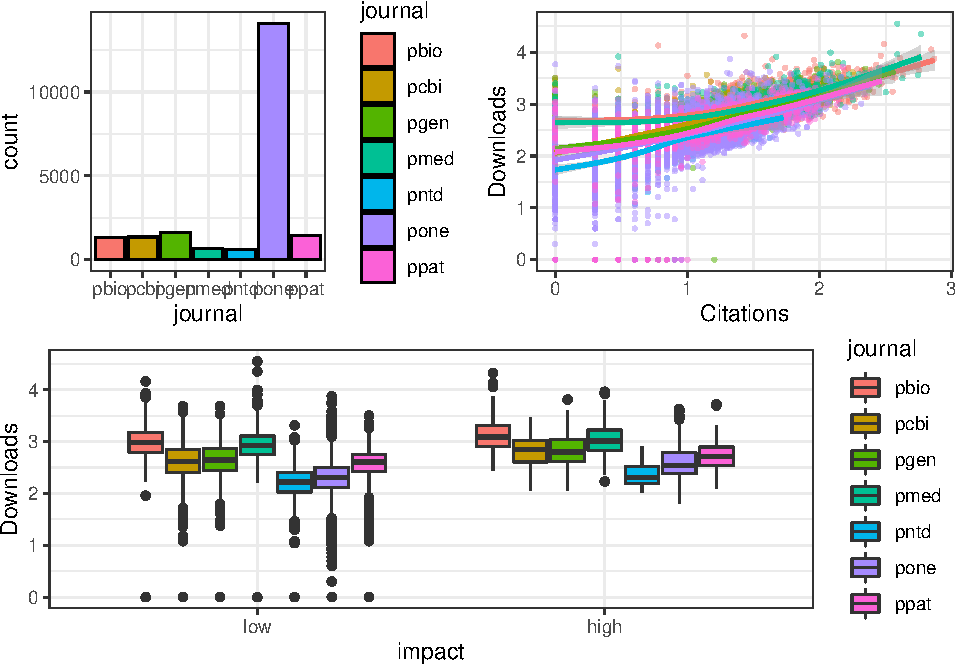
\includegraphics{Notes_files/figure-latex/unnamed-chunk-48-1.pdf}

\hypertarget{the-cowplot-package}{%
\subsection*{\texorpdfstring{The \texttt{cowplot} package}{The cowplot package}}\label{the-cowplot-package}}
\addcontentsline{toc}{subsection}{The \texttt{cowplot} package}

We can also arrange these plots using the \texttt{plot\_grid()} function.

\begin{Shaded}
\begin{Highlighting}[]
\KeywordTok{library}\NormalTok{(cowplot)}

\KeywordTok{plot_grid}\NormalTok{(plot1, plot2, plot3)}
\end{Highlighting}
\end{Shaded}

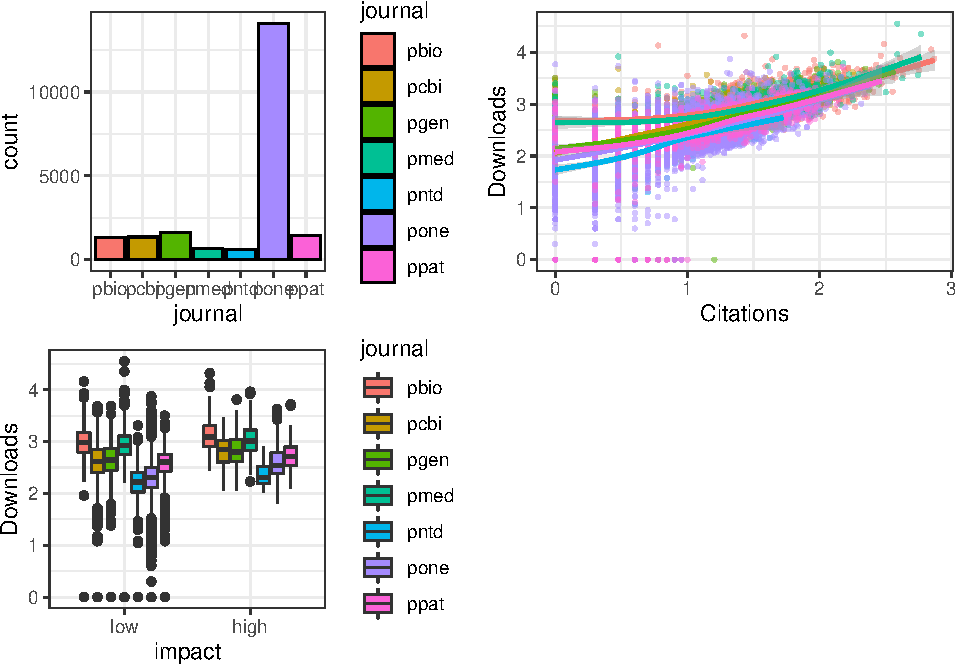
\includegraphics{Notes_files/figure-latex/unnamed-chunk-49-1.pdf}

\begin{Shaded}
\begin{Highlighting}[]
\NormalTok{row1 <-}\StringTok{ }\KeywordTok{plot_grid}\NormalTok{(plot1, plot2, }\DataTypeTok{labels =} \KeywordTok{c}\NormalTok{(}\StringTok{"A"}\NormalTok{, }\StringTok{"B"}\NormalTok{), }\DataTypeTok{nrow =} \DecValTok{1}\NormalTok{)}
\NormalTok{row2 <-}\StringTok{ }\KeywordTok{plot_grid}\NormalTok{(plot3, }\DataTypeTok{labels =} \KeywordTok{c}\NormalTok{(}\StringTok{"C"}\NormalTok{), }\DataTypeTok{nrow =} \DecValTok{1}\NormalTok{)}

\KeywordTok{plot_grid}\NormalTok{(row1, row2, }\DataTypeTok{nrow =} \DecValTok{2}\NormalTok{)}
\end{Highlighting}
\end{Shaded}

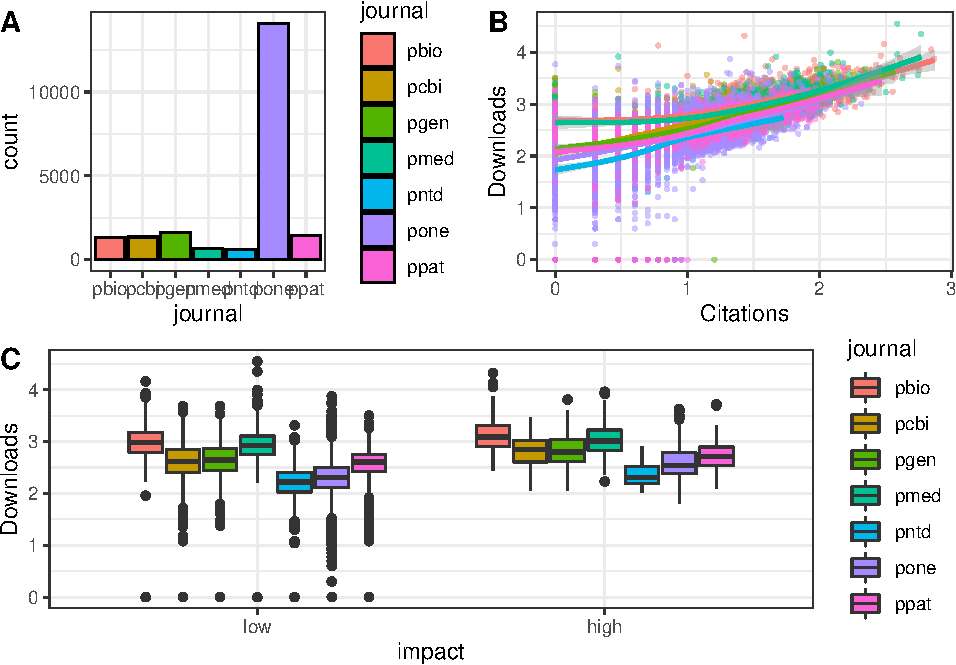
\includegraphics{Notes_files/figure-latex/unnamed-chunk-49-2.pdf}

\hypertarget{saving-plots}{%
\subsection{Saving plots}\label{saving-plots}}

The easiest way to save a plot is using the \texttt{ggsave()} function.

\begin{center}\rule{0.5\linewidth}{0.5pt}\end{center}

\hypertarget{exercise-8.1}{%
\subsection*{Exercise 8.1}\label{exercise-8.1}}
\addcontentsline{toc}{subsection}{Exercise 8.1}

Using the publication dataset we've been using, complete the following tasks.

\begin{enumerate}
\def\labelenumi{\arabic{enumi}.}
\tightlist
\item
  Generate a table containing the mean and standard error of the number of tweets per journal. It should look something like this:
\end{enumerate}

\begin{verbatim}
## # A tibble: 7 x 4
##   journal   num   mean     sem
##   <fct>   <int>  <dbl>   <dbl>
## 1 pbio     1325 0.0581 0.0202 
## 2 pcbi     1351 0.127  0.0522 
## 3 pgen     1619 0.0655 0.0204 
## 4 pmed      643 0.311  0.188  
## 5 pntd      621 0.0258 0.00906
## 6 pone    14078 0.493  0.0345 
## 7 ppat     1459 0.0260 0.00881
\end{verbatim}

\begin{enumerate}
\def\labelenumi{\arabic{enumi}.}
\setcounter{enumi}{1}
\tightlist
\item
  Use this table to create a bar plot of mean tweets per journal, including standard error. It should look something like this:
\end{enumerate}

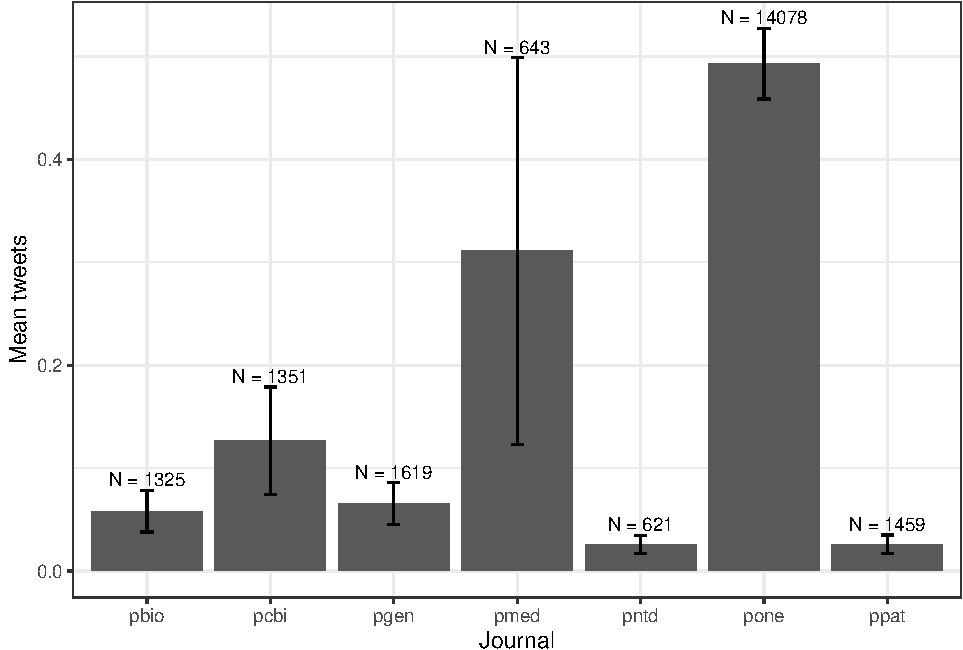
\includegraphics{Notes_files/figure-latex/unnamed-chunk-51-1.pdf}

Hint: you will want to use the function \texttt{geom\_errorbar()} to add the error bars.

\begin{enumerate}
\def\labelenumi{\arabic{enumi}.}
\setcounter{enumi}{2}
\tightlist
\item
  Create a box plot of the number of citations per journal (ie. the variable wosCountThur2011). Colour the journals using the \texttt{Accent} palette from the \texttt{RColorBrewer} package. It should look something like this:
\end{enumerate}

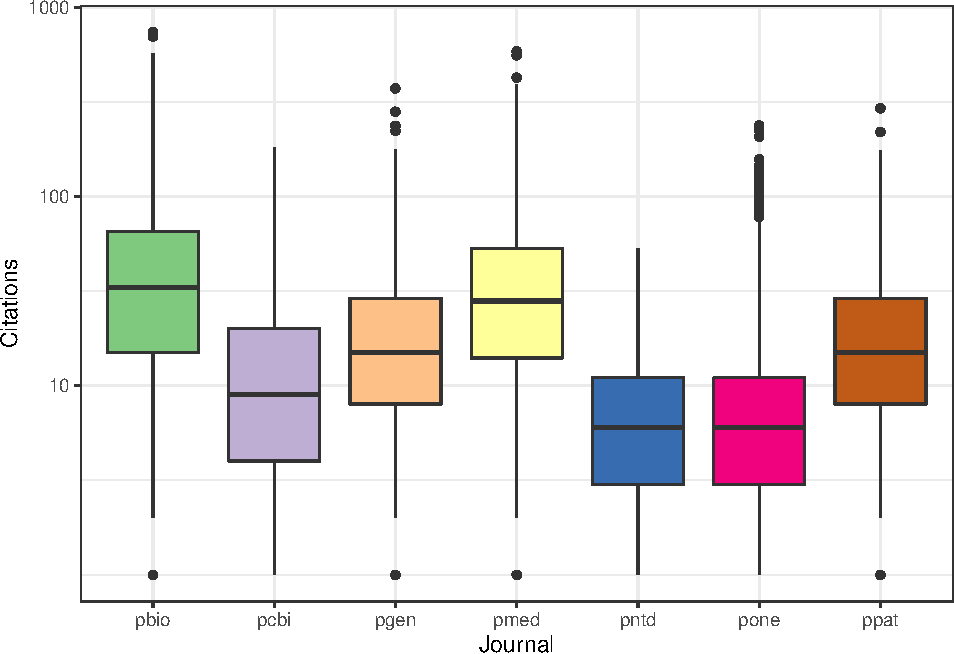
\includegraphics{Notes_files/figure-latex/unnamed-chunk-52-1.pdf}

\begin{enumerate}
\def\labelenumi{\arabic{enumi}.}
\setcounter{enumi}{3}
\tightlist
\item
  Generate a plot that shows the number of downloads over time, coloured by journal. It should look something like this:
\end{enumerate}

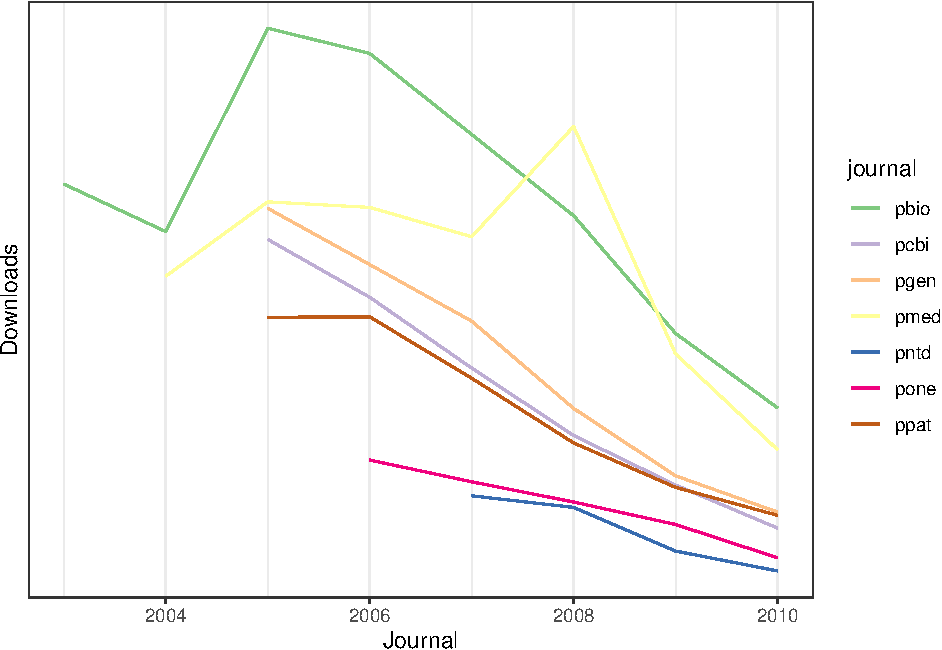
\includegraphics{Notes_files/figure-latex/unnamed-chunk-53-1.pdf}

\begin{center}\rule{0.5\linewidth}{0.5pt}\end{center}

\hypertarget{additional-resources}{%
\section{Additional Resources}\label{additional-resources}}

\url{http://www.sthda.com/english/wiki/be-awesome-in-ggplot2-a-practical-guide-to-be-highly-effective-r-software-and-data-visualization}

\url{http://r-statistics.co/Top50-Ggplot2-Visualizations-MasterList-R-Code.html}

\begin{itemize}
\tightlist
\item
  Mailing list: \url{http://groups.google.com/group/ggplot2}
\item
  Wiki: \url{https://github.com/hadley/ggplot2/wiki}
\item
  Website: \url{http://had.co.nz/ggplot2/}
\item
  StackOverflow: \url{http://stackoverflow.com/questions/tagged/ggplot}
\end{itemize}

Cheatsheet

\hypertarget{advanced-rmarkdown}{%
\chapter{Advanced Rmarkdown}\label{advanced-rmarkdown}}

So far we have use default settings to create our Rmarkdown documents. Lets \textbf{prettify} our documents!!

\hypertarget{yaml-options-for-html-documents}{%
\section{YAML options for HTML documents}\label{yaml-options-for-html-documents}}

As we just mentioned before, Markdown was originally designed for HTML output, so it may not be surprising that the HTML format has the richest features among all output formats. We recommend that you read this full section before you learn other output formats, because other formats have several features in common with the HTML document format, and we will not repeat these features in the corresponding sections.

To create an HTML document from R Markdown, you specify the html\_document output format in the YAML metadata of your document:

\begin{Shaded}
\begin{Highlighting}[]
\OperatorTok{---}
\NormalTok{title}\OperatorTok{:}\NormalTok{ first_markdown}
\NormalTok{author}\OperatorTok{:}\NormalTok{ ME ME}
\NormalTok{date}\OperatorTok{:}\NormalTok{ March }\DecValTok{22}\OperatorTok{,} \DecValTok{2005}
\NormalTok{output}\OperatorTok{:}\NormalTok{ html_document}
\OperatorTok{---}
\end{Highlighting}
\end{Shaded}

Lets add themes and highlight options

\begin{Shaded}
\begin{Highlighting}[]
\NormalTok{title}\OperatorTok{:}\NormalTok{ first_markdown}
\NormalTok{author}\OperatorTok{:}\NormalTok{ ME ME}
\NormalTok{date}\OperatorTok{:}\NormalTok{ March }\DecValTok{22}\OperatorTok{,} \DecValTok{2005}
\NormalTok{output}\OperatorTok{:} 
\NormalTok{  html_document}\OperatorTok{:}
\NormalTok{    theme}\OperatorTok{:}\NormalTok{ yeti}
\NormalTok{    highlight}\OperatorTok{:}\NormalTok{ kate}
\end{Highlighting}
\end{Shaded}

Now lets add a table of contents

\begin{Shaded}
\begin{Highlighting}[]

\NormalTok{title}\OperatorTok{:}\NormalTok{ first_markdown}
\NormalTok{author}\OperatorTok{:}\NormalTok{ ME ME}
\NormalTok{date}\OperatorTok{:}\NormalTok{ March }\DecValTok{22}\OperatorTok{,} \DecValTok{2005}
\NormalTok{output}\OperatorTok{:} 
\NormalTok{  html_document}\OperatorTok{:}
\NormalTok{    theme}\OperatorTok{:}\NormalTok{ yeti}
\NormalTok{    highlight}\OperatorTok{:}\NormalTok{ kate}
\NormalTok{    toc}\OperatorTok{:} \KeywordTok{true}
\NormalTok{    toc_float}\OperatorTok{:} 
\NormalTok{      collapsed}\OperatorTok{:} \KeywordTok{false}
\NormalTok{    toc_depth}\OperatorTok{:} \DecValTok{4}
\end{Highlighting}
\end{Shaded}

if you want to hide your code

\begin{Shaded}
\begin{Highlighting}[]
\NormalTok{title}\OperatorTok{:}\NormalTok{ first_markdown}
\NormalTok{author}\OperatorTok{:}\NormalTok{ ME ME}
\NormalTok{date}\OperatorTok{:}\NormalTok{ March }\DecValTok{22}\OperatorTok{,} \DecValTok{2005}
\NormalTok{output}\OperatorTok{:} 
\NormalTok{  html_document}\OperatorTok{:}
\NormalTok{    theme}\OperatorTok{:}\NormalTok{ yeti}
\NormalTok{    highlight}\OperatorTok{:}\NormalTok{ kate}
\NormalTok{    toc}\OperatorTok{:} \KeywordTok{true}
\NormalTok{    toc_float}\OperatorTok{:} 
\NormalTok{      collapsed}\OperatorTok{:} \KeywordTok{false}
\NormalTok{    toc_depth}\OperatorTok{:} \DecValTok{4}
\NormalTok{    code_folding}\OperatorTok{:}\NormalTok{ hide}
\end{Highlighting}
\end{Shaded}

A way to add custom css

\begin{Shaded}
\begin{Highlighting}[]
\NormalTok{title}\OperatorTok{:}\NormalTok{ first_markdown}
\NormalTok{author}\OperatorTok{:}\NormalTok{ ME ME}
\NormalTok{date}\OperatorTok{:}\NormalTok{ March }\DecValTok{22}\OperatorTok{,} \DecValTok{2005}
\NormalTok{output}\OperatorTok{:} 
\NormalTok{  html_document}\OperatorTok{:}
\NormalTok{    theme}\OperatorTok{:}\NormalTok{ yeti}
\NormalTok{    highlight}\OperatorTok{:}\NormalTok{ kate}
\NormalTok{    css}\OperatorTok{:} \VariableTok{styles}\NormalTok{.}\AttributeTok{css}
\NormalTok{    toc}\OperatorTok{:} \KeywordTok{true}
\NormalTok{    toc_float}\OperatorTok{:} 
\NormalTok{      collapsed}\OperatorTok{:} \KeywordTok{false}
\NormalTok{    toc_depth}\OperatorTok{:} \DecValTok{4}
\NormalTok{    code_folding}\OperatorTok{:}\NormalTok{ hide}
\end{Highlighting}
\end{Shaded}

\hypertarget{cool-stuff-in-rmarkdown}{%
\section{Cool stuff in Rmarkdown}\label{cool-stuff-in-rmarkdown}}

\#\#\# CHEATSHEET
This cheat sheet has all the details on how to add figures, links, bullets, headings and tables in Rmarkdown!
\href{img/rmarkdown-2.0.pdf}{}
\#\#\# Making cools tables in Rmarkdown from R code
Tables generated from your R code are very useful to share modified output with other users.
Simplest tables in markdown can be generated using the kable function but these table are static and to be honest boring!
\#\#\#\# A kable table

\begin{verbatim}
library(knitr)
kable(cars)
\end{verbatim}

\begin{Shaded}
\begin{Highlighting}[]
\NormalTok{knitr}\OperatorTok{::}\KeywordTok{kable}\NormalTok{(cars)}
\end{Highlighting}
\end{Shaded}

\begin{tabular}{r|r}
\hline
speed & dist\\
\hline
4 & 2\\
\hline
4 & 10\\
\hline
7 & 4\\
\hline
7 & 22\\
\hline
8 & 16\\
\hline
9 & 10\\
\hline
10 & 18\\
\hline
10 & 26\\
\hline
10 & 34\\
\hline
11 & 17\\
\hline
11 & 28\\
\hline
12 & 14\\
\hline
12 & 20\\
\hline
12 & 24\\
\hline
12 & 28\\
\hline
13 & 26\\
\hline
13 & 34\\
\hline
13 & 34\\
\hline
13 & 46\\
\hline
14 & 26\\
\hline
14 & 36\\
\hline
14 & 60\\
\hline
14 & 80\\
\hline
15 & 20\\
\hline
15 & 26\\
\hline
15 & 54\\
\hline
16 & 32\\
\hline
16 & 40\\
\hline
17 & 32\\
\hline
17 & 40\\
\hline
17 & 50\\
\hline
18 & 42\\
\hline
18 & 56\\
\hline
18 & 76\\
\hline
18 & 84\\
\hline
19 & 36\\
\hline
19 & 46\\
\hline
19 & 68\\
\hline
20 & 32\\
\hline
20 & 48\\
\hline
20 & 52\\
\hline
20 & 56\\
\hline
20 & 64\\
\hline
22 & 66\\
\hline
23 & 54\\
\hline
24 & 70\\
\hline
24 & 92\\
\hline
24 & 93\\
\hline
24 & 120\\
\hline
25 & 85\\
\hline
\end{tabular}

\#\#\#\# A DT table

\begin{verbatim}
library(DT)
datatable(cars)
\end{verbatim}

\begin{Shaded}
\begin{Highlighting}[]
\KeywordTok{library}\NormalTok{(DT)}
\KeywordTok{datatable}\NormalTok{(cars)}
\end{Highlighting}
\end{Shaded}

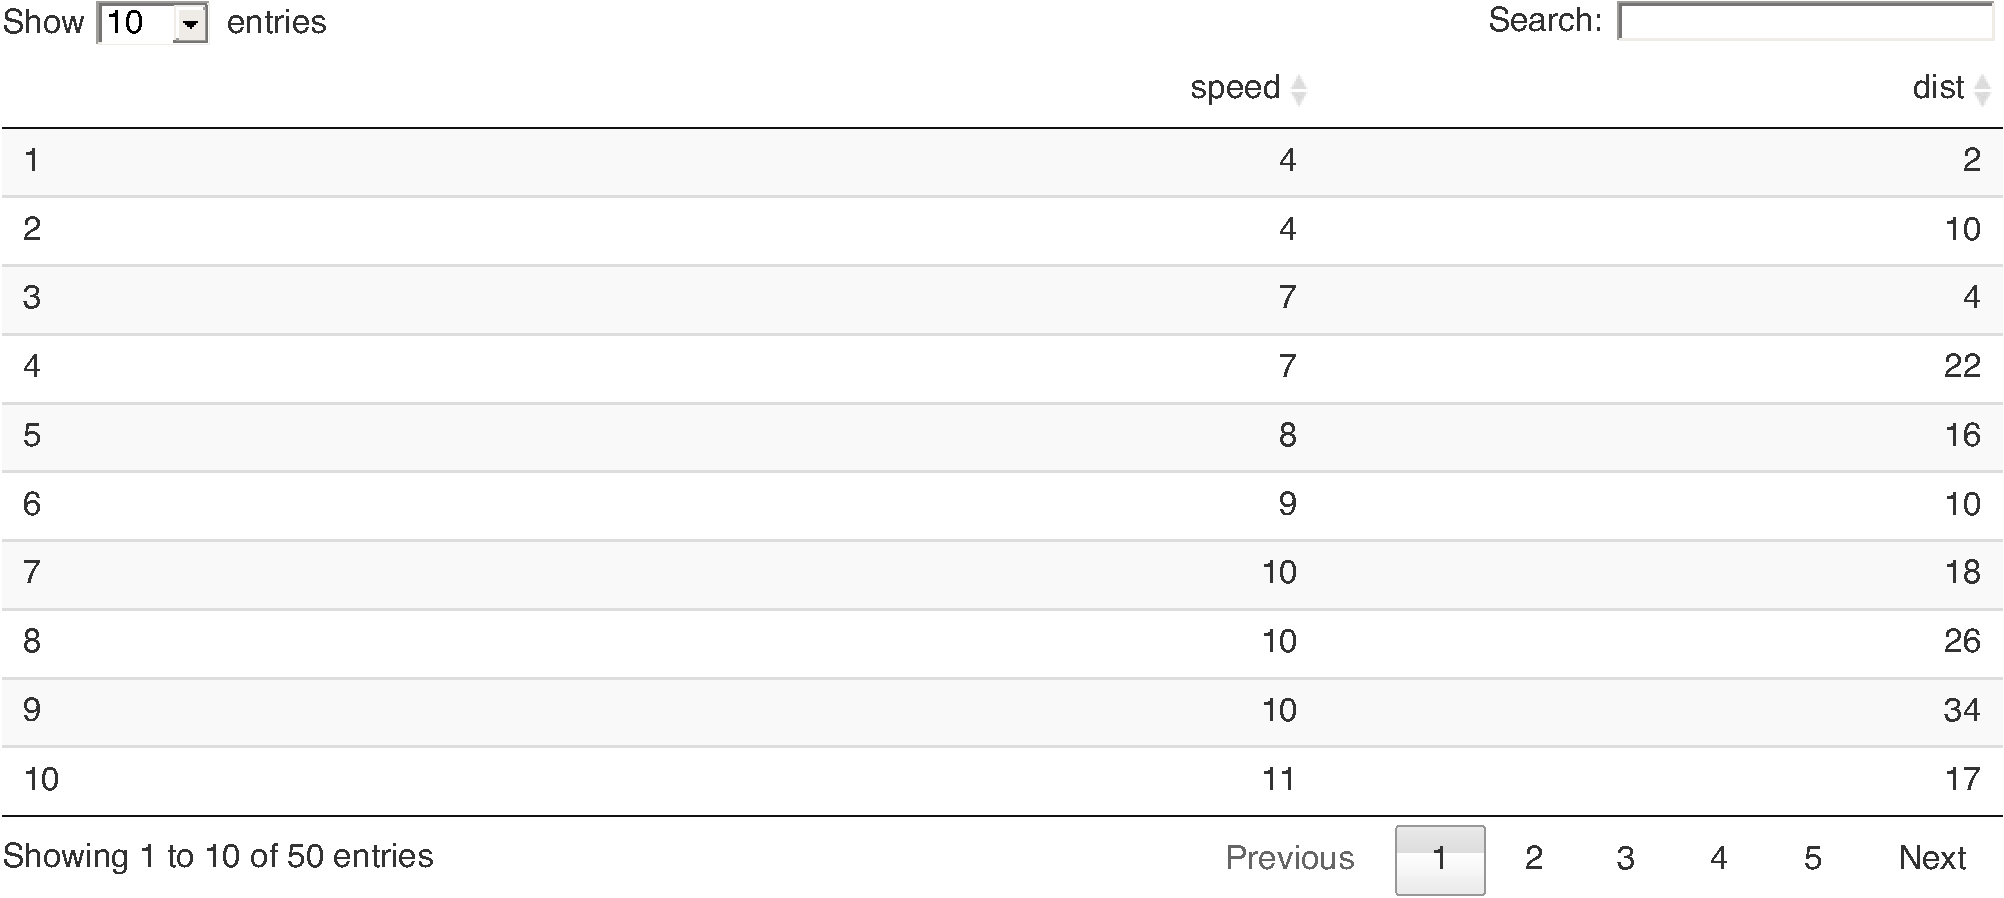
\includegraphics{Notes_files/figure-latex/unnamed-chunk-60-1.pdf}

\#\#\#\# DT table with download options

\begin{verbatim}
library(DT)
datatable(cars,
  extensions = 'Buttons', options = list(
    dom = 'Bfrtip',
    buttons = c('copy', 'print','csv', 'excel')
  )
)
\end{verbatim}

\begin{Shaded}
\begin{Highlighting}[]
\KeywordTok{library}\NormalTok{(DT)}
\KeywordTok{datatable}\NormalTok{(cars,}
           \DataTypeTok{extensions =} \StringTok{'Buttons'}\NormalTok{, }\DataTypeTok{options =} \KeywordTok{list}\NormalTok{(}
    \DataTypeTok{dom =} \StringTok{'Bfrtip'}\NormalTok{,}
    \DataTypeTok{buttons =} \KeywordTok{c}\NormalTok{(}\StringTok{'copy'}\NormalTok{, }\StringTok{'print'}\NormalTok{,}\StringTok{'csv'}\NormalTok{, }\StringTok{'excel'}\NormalTok{)}
\NormalTok{    )}
\NormalTok{)}
\end{Highlighting}
\end{Shaded}

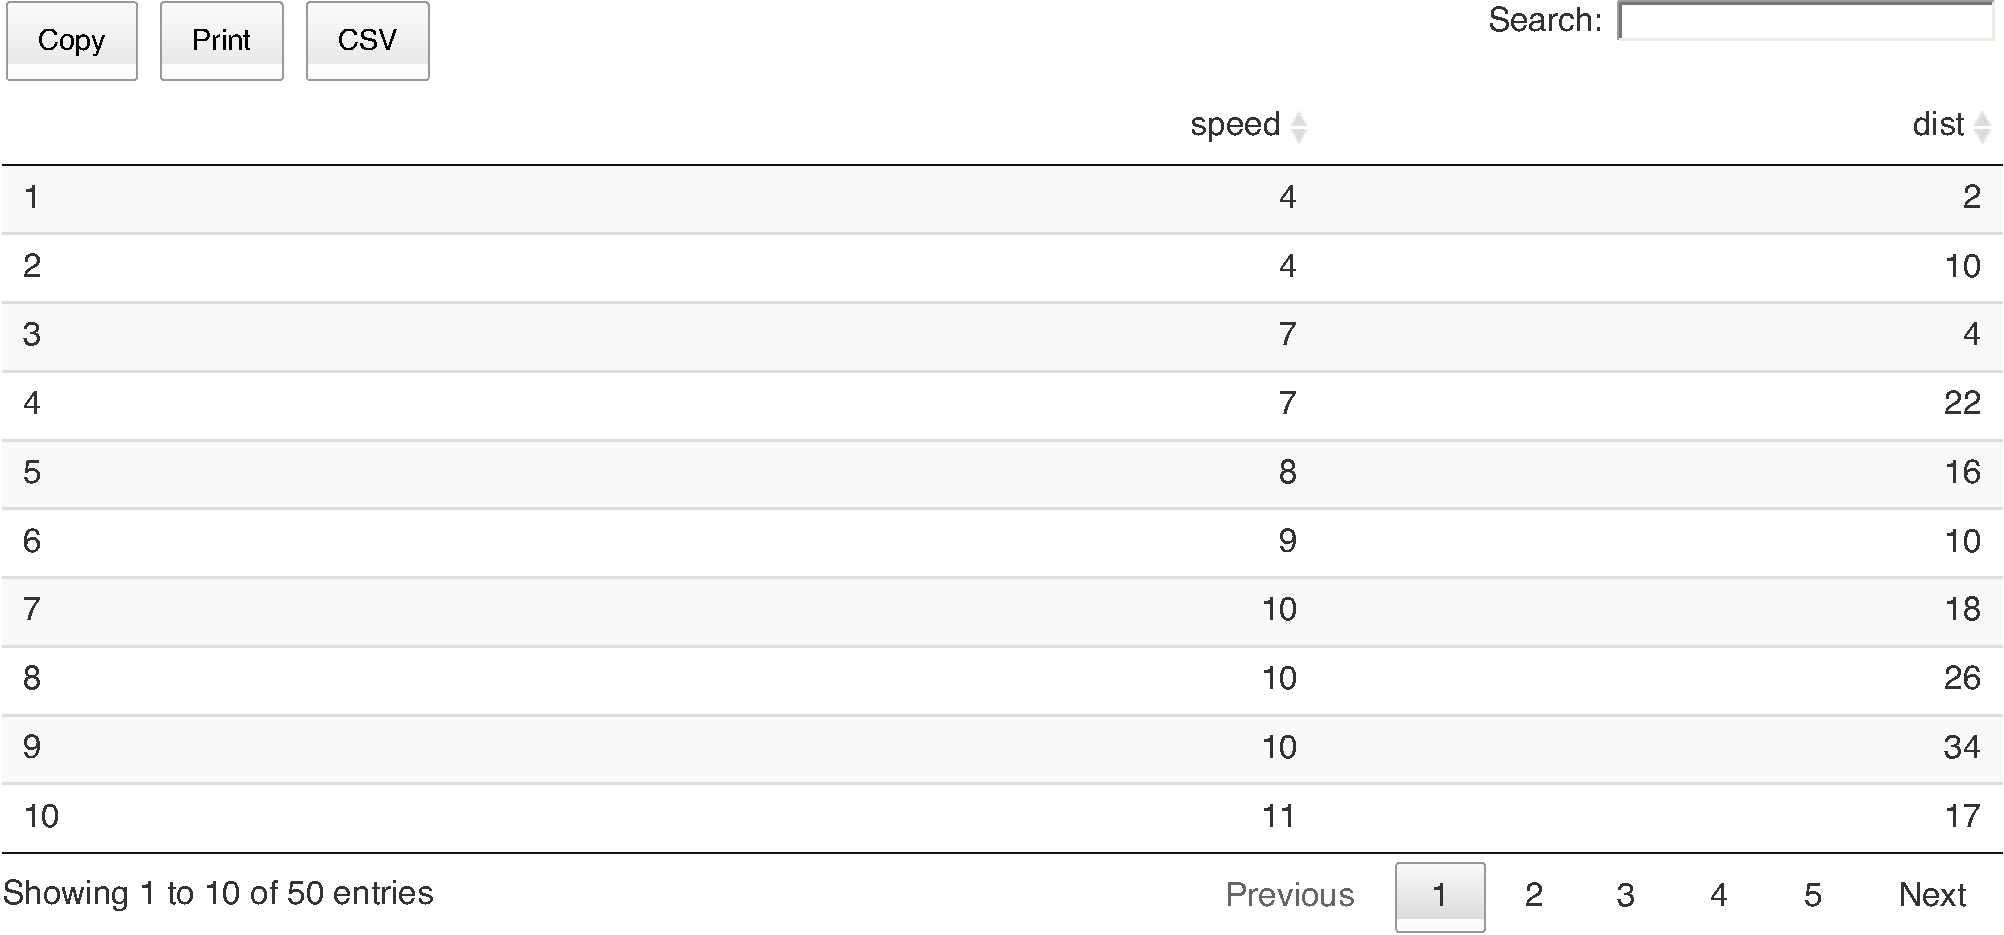
\includegraphics{Notes_files/figure-latex/unnamed-chunk-61-1.pdf}

\hypertarget{making-tabs-in-rmarkdown}{%
\subsection{Making tabs in Rmarkdown}\label{making-tabs-in-rmarkdown}}

You can organize content using tabs by applying the .tabset class attribute to headers within a document. This will cause all sub-headers of the header with the .tabset attribute to appear within tabs rather than as standalone sections. For example:

\begin{verbatim}
## Quarterly Results {.tabset}

### By Product

(tab content)

### By Region

(tab content)
\end{verbatim}

You can also specify two additional attributes to control the appearance and behavior of the tabs. The .tabset-fade attribute causes the tabs to fade in and out when switching between tabs. The .tabset-pills attribute causes the visual appearance of the tabs to be ``pill'' rather than traditional tabs. For example:

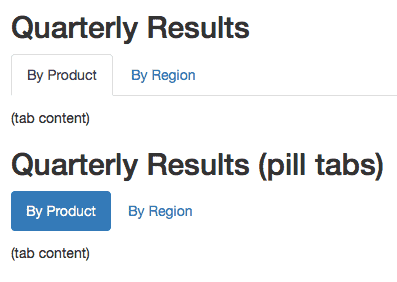
\includegraphics{img/tabset.png}

\hypertarget{rmarkdown-to-html-conversion}{%
\subsection{Rmarkdown to HTML conversion}\label{rmarkdown-to-html-conversion}}

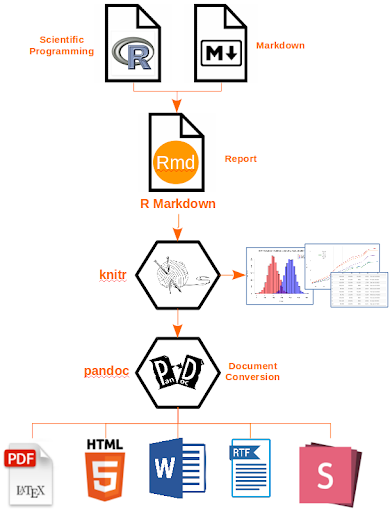
\includegraphics{img/rmarkdown_html.png}

\hypertarget{html-and-css-basics}{%
\section{HTML and CSS basics}\label{html-and-css-basics}}

HTML, \textbf{HyperText Markup Language}, gives content structure and meaning by defining that content as, for example, headings, paragraphs, or images. CSS, ** Cascading Style Sheets**, is a presentation language created to style the appearance of content---using, for example, fonts or colors.

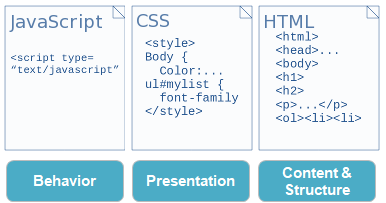
\includegraphics{img/js_css_html.png}

Lets look at the following examples

\href{data/case_study_default.html}{Simple html generated from Rmarkdown}

\href{data/case_study_theme.html}{Simple html styled by css from themes}

\href{data/case_study_extreme.html}{Simple html styled by custom css}

\#\#\# HTML

\begin{verbatim}
<!DOCTYPE html>
<html>
<body>

<h1>My First Heading</h1>
<p>My first paragraph.</p>

</body>
</html>
\end{verbatim}

\#\#\#\#Output:

My First Heading

My first paragraph.

You will not have to worry about html too much in Rmarkdown. However,
once in a while you might want to add color to some text or other simple things:

\begin{verbatim}
<p style="color:tomato">My first paragraph.</p>
\end{verbatim}

\textbf{Output}

My first paragraph.

\begin{verbatim}
<p style="color:tomato;font-family:verdana">My first paragraph.</p>
\end{verbatim}

\textbf{Output}

My first paragraph.

I use a lot which means adds a single break meaning a extra empty line

There are options for highlighting, bold, italic etc

To learn more html go to \url{https://www.w3schools.com/default.asp} .

\hypertarget{css}{%
\subsection{CSS}\label{css}}

\begin{itemize}
\tightlist
\item
  CSS stands for Cascading Style Sheets
\item
  CSS describes how HTML elements are to be displayed on screen, paper, or in other media
\item
  CSS saves a lot of work. It can control the layout of multiple web pages all at once
\item
  External stylesheets are stored in CSS files
\end{itemize}

\hypertarget{css-syntax}{%
\subsubsection{CSS Syntax}\label{css-syntax}}

A CSS rule-set consists of a selector and a declaration block:

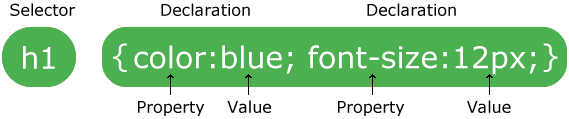
\includegraphics{img/css_selector.png}

\begin{itemize}
\item
  The selector points to the HTML element you want to style.
\item
  The declaration block contains one or more declarations separated by semicolons.
\item
  Each declaration includes a CSS property name and a value, separated by a colon.
\item
  Multiple CSS declarations are separated with semicolons, and declaration blocks are surrounded by curly braces.
\end{itemize}

p \{
color: red;
text-align: center;
\}

\begin{itemize}
\tightlist
\item
  p is a selector in CSS (it points to the HTML element you want to style:

  ).
\item
  color is a property, and red is the property value
\item
  text-align is a property, and center is the property value
\end{itemize}

To learn more visit \url{https://www.w3schools.com/css/css_syntax.asp}

\hypertarget{exercise-6}{%
\subsubsection*{Exercise}\label{exercise-6}}
\addcontentsline{toc}{subsubsection}{Exercise}

Start a new Rmarkdown file for your project. In the same folder, create a styles.css file.In this file write CSS code to change the color of h1 and h2 to one you like. Now link this file to your project Rmarkdown file.

\hypertarget{project}{%
\chapter{Project}\label{project}}

\hypertarget{setup-1}{%
\section{Setup}\label{setup-1}}

Please download the data folder from Dropbox

\hypertarget{task-1}{%
\section{Task 1}\label{task-1}}

\begin{enumerate}
\def\labelenumi{\arabic{enumi}.}
\tightlist
\item
  Create a new R Project for this case study.
\item
  Create a new Rmd file to complete your project.
\item
  Change the auther name of the .Rmd file to your name and add today's date.
\item
  Read in all the files in the data folder into single dataframe. Hint: Use for loops to read in all the files.Functions that can be helpful : list.files,read\_csv,rbind,data.frame(NULL)
\end{enumerate}

\hypertarget{task-2}{%
\section{Task 2}\label{task-2}}

\begin{enumerate}
\def\labelenumi{\arabic{enumi}.}
\tightlist
\item
  Write a function that takes a dataframe as input and if present, converts Monthin to 4 yearly quaters and add an extra column to your dataframe/tibble called Quarters with 4 levels: Q1,Q2,Q3 and, Q4.
\end{enumerate}

\begin{itemize}
\tightlist
\item
  When Month is Jan-Mar, Quarter = ``Q1''
\item
  When Month is Apr-Jun, Quarter = ``Q2''
\item
  When Month is Jul-Sep, Quarter = ``Q3''
\item
  When Month is Oct-Dec, Quarter = ``Q4''
\end{itemize}

Hint: Use mutate and case\_when(), \%in\% and stop() function

\hypertarget{task-3}{%
\section{Task 3}\label{task-3}}

\begin{enumerate}
\def\labelenumi{\arabic{enumi}.}
\tightlist
\item
  Generate a bar plot that shows the number of transactions of each card type per quarter. (The card type is called \texttt{Factor\_C}).
\item
  Place the legend at the top of the plot.
\item
  Remove the x axis labels and tick marks.
\item
  Colour the card types using a palette of your choice from the RColorBrewer package.
\end{enumerate}

\hypertarget{task-4}{%
\section{Task 4}\label{task-4}}

\begin{enumerate}
\def\labelenumi{\arabic{enumi}.}
\tightlist
\item
  Use the \texttt{colorRampPalette()} function to generate a colour ramp between any two colours.
\item
  Plot the distribution (ie. histogram) of Account ID for each quarter.
\item
  Add a density line.
\item
  Remove the legend.
\item
  Plot the density lines only for Account ID for each month on the same plot.
\end{enumerate}

\hypertarget{task-5}{%
\section{Task 5}\label{task-5}}

\begin{enumerate}
\def\labelenumi{\arabic{enumi}.}
\tightlist
\item
  Use the dplyr functions to generate a dataframe containing the proportion of Approved and Declined transactions for each card type.
\item
  Generate a bar plot showing the proportion for each card type.
\item
  Flip the coordinates so that each card type is a row.
\end{enumerate}

\hypertarget{task-6}{%
\section{Task 6}\label{task-6}}

Generate an html report of all the above tasks using R Markdown. Use \href{data/case_study_theme.html}{this file} as a guide.

\hypertarget{usefull-links}{%
\chapter{Usefull links}\label{usefull-links}}

\hypertarget{cheatsheets}{%
\section{CheatSheets}\label{cheatsheets}}

This is a useful set of cheat sheets that can be handy for you.

\begin{enumerate}
\def\labelenumi{\arabic{enumi}.}
\tightlist
\item
  \href{img/data-import.pdf}{Importing data}
\item
  \href{img/rmarkdown-2.0.pdf}{rmarkdown}
\item
  \href{img/ggplot2-cheatsheet.pdf}{ggplot2}
\end{enumerate}

Packages not discussed in the workshop but worth a try!

\begin{enumerate}
\def\labelenumi{\arabic{enumi}.}
\tightlist
\item
  \href{img/factors.pdf}{forcats}
\item
  \href{img/purrr.pdf}{Purrr}
\item
  \href{img/strings.pdf}{strings}
\end{enumerate}

These notes are modified from and at some places directly taken from \url{https://jdblischak.github.io/r-intermediate-altmetrics/}

  \bibliography{book.bib,packages.bib}

\end{document}
